%!TEX root = ../../thesis.tex
\define{\chapterpath}{\allchapterspath/limitations}
\define{\imgpath}{\chapterpath/img}

%
\chapter{Limitations, Extensions and Derivatives}
\label{chapter:limitations}
\minitoc

In the previous chapters, we described an algorithm that allow a robot to learn a new task by interacting with a human partners without defining in advance how the signals of the user maps to the meaning used by the learning agent. We tested this algorithm on two domains, a pick and place scenario using speech commands, and a reaching task scenario using EEG signals. We demonstrated the use of our system online and with real subjects using their brain to assess agent's action with respect to a final desired position.

However a number of assumptions and constraints have been defined. In this chapter we will detail a number of those limitations, discuss the possibility to overcome them and provide small experiments to demonstrate our ideas. 

In section~\ref{chapter:limitiations:simplevsmatching} we compare the performance of Equation~\ref{eq:matchingfilter} and Equation~\ref{eq:matchingfiltercrossvalidation} defined in chapter~\ref{chapter:lfui}. We show that corrrecting the classifier prediction given our knowledge about one classifier (Equation~\ref{eq:matchingfiltercrossvalidation}) makes our algortihm more robust than relying on the raw classifier outputs (Equation~\ref{eq:matchingfilter}).

In section~\ref{chapter:limitations:wordlproperties}, we present preliminary studies on how different properties of the world impacts the efficiency of several planning methods. We specifically study the impact of the size and the maze like properties. This study will highlight the fact that our uncertainty based planning method allow to identify the correct task with best performance in a few types of problems. However we will see that, by not considering the performance on the task itself during the exploration, for some problems our method lacks of efficiency with respect to solving the task as fast as possible.

In section~\ref{chapter:limitations:overlap} we introduce an other method to identify the first target based on models overlap, we present online results with real subjects in a BCI scenario, and show the limitation of this new method to identifying a sequence of multiple tasks.

In section~\ref{chapter:limitations:framegeneric} we insist again on the fact that an interaction frame is not limited to the straightforward meaning correspond we assumed (feedback and guidance), and do not requires the robot to know how to perform a task.

In section~\ref{chapter:limitations:continousstate}, we address the problem of continuous state space, and show that our method is not impacted by the continuous aspect of the problem. Indeed, as our method, when considering a simple frame, only requires to known the policy for each task, we can rely on any algorithm that computes a policy for continuous states given a pre-defined task.

In section~\ref{chapter:limitations:continoushypothesis}, we release the assumption of a finite set of task and rely on a particle filter based method to dynamically update a finite set of hypothesis. We show that sampling actively the new task, as well as selecting actively the next visited state, significantly improves the final performance of our method.

In section~\ref{chapter:limitations:framehypothesis}, we release the assumption that the interaction frame is known and consider the agent as access to a finite number of hypothetic interaction frames. We illustrated this problem in a simple scenario line world scenario. And present results from simulated experiments that demonstrate the ability our method to not only learn the task and the signal to meaning mapping, but also the interaction protocol used by the teacher.

In section~\ref{chapter:limitations:userstudies}, we discuss the need for conducting user studies in more complex domain to evaluate the scalability, efficiency, and acceptability of our method.

In section~\ref{chapter:limitations:proof}, we pinpoint the importance of understanding the properties of our algorithm, and to be able to have some certitude about its convergence and accuracy properties; and we propose a minimalist proof of for our algortihm.

Finally in section~\ref{chapter:limitations:discussion}, we discuss a number of limitations that were not addressed in this work and that are not straightforward to solve given our context. Such as using continuous actions or learning new meanings.

%%%%%%%%%%%%%%%%%%%%%%%%%%%%%%%%%%%%%%%%%%%%%%
%%%%%%%%%%%%%%%%%%%%%%%%%%%%%%%%%%%%%%%%%%%%%%
%%%%%%%%%%%%%%%%%%%%%%%%%%%%%%%%%%%%%%%%%%%%%%
%%%%%%%%%%%%%%%%%%%%%%%%%%%%%%%%%%%%%%%%%%%%%%
%%%%%%%%%%%%%%%%%%%%%%%%%%%%%%%%%%%%%%%%%%%%%%
%!TEX root = ../../thesis.tex

\section{Why should we correct classifiers prediction}
\label{chapter:limitiations:simplevsmatching}


we compared the result between 
\ref{eq:matchingfilter}
and
\ref{eq:matchingfiltercrossvalidation} 

Still, this last approach is not taking into account the quality of the classifier itself before taking into account its prediction. By this we ask the question of knowing how reliable the prediction of the classifier are? A common method to evaluate the uncertainty on the classifier prediction is to use a cross-validation procedure (see chapter~\ref{chapter:introduction:supervised}) to estimate the confusion matrix associated to the classifier. Such confusion matrix allow to infer the conditional probability of one label given the label prediction from the classifier $p(l^{cc} = l_k| l^c = l_q, \theta)$, for every combination of $k$ and $q$ in $1, \ldots, L$. Where $l^{cc}$ is the corrected, or ``temperated'', label predicted by the classifier given our estimates, our past experience, on the quality of its prediction using the cross validation procedure.

We consider the same setting as for the experiments described in chapter~\ref{chapter:bci:EEGsignals} and used our 2 dimensionnal dataset of different quality as presented in chapter~\ref{chapter:planning:artificialsignals}. We ran 500 simulations for each method.


% nSim =

%   Columns 1 through 3

%    104    98   123
%    115    96    90

%   Columns 4 through 5

%     86    89
%     83   117


\paragraph{Time to first task} Figure~\ref{fig:timefirst_simplevsmatching} compares the number of iterations needed to identify the first time with confidence between our general method (matching), or using the information that ``incorrect'' signals are more powerful than the ``correct'' (power), or both method combined (power matching). The use of the power information affects the performances for the low quality dataset. For datasets of low quality, while the time to first seems more advantageous for the method using the power information, most of the estimated task are erroneous (see Figure~\ref{tab:errorTaskRatio}) which makes the use of the power information critical for such low quality data. However those errors occurs for very low quality datasets, which are not the main target of our algorithm. For such data it would be better to change the representation of the signal or the classifier used. For the datasets of higher quality, the power information allow to slightly speed up the learning compared to our method (matching) which do not rely on known information. 

\begin{figure}[!ht]
\centering
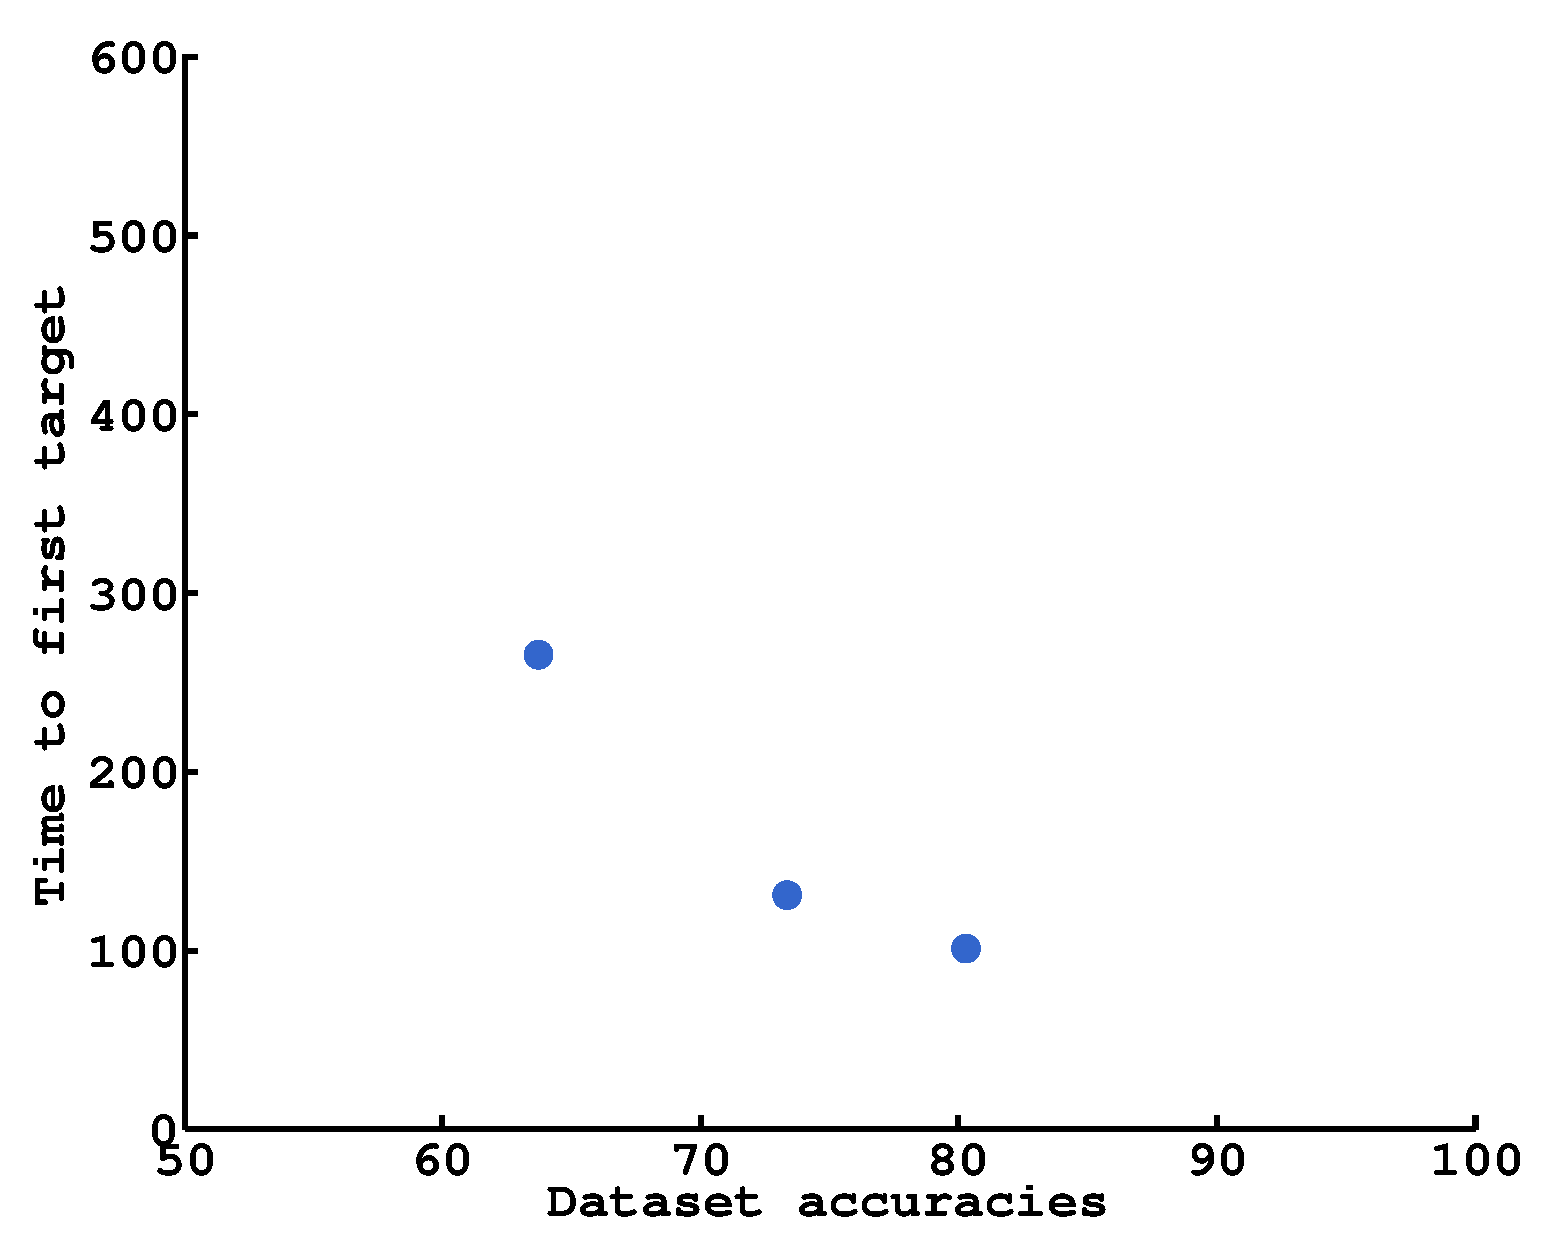
\includegraphics[width=\plotsize\columnwidth]{\imgpath/simplevsmatching/timefirst.eps}
\caption{Number of steps to complete first task with EEG data. Comparison between Equation~\ref{eq:matchingfilter} (simple matching) and Equation~\ref{eq:matchingfiltercrossvalidation} (matching), where the latter correct the prediction of the classifier given the estimation of its confusion matrix. 
% The use of the power information affects the performance for the low quality dataset. For datasets of low quality, while the time to first seems more advantageous for the method using the power information, most of the estimated task are erroneous (see Figure~\ref{tab:errorTaskRatio}) which makes the use of the power information critical for such low quality data. However those errors occurs for very low quality datasets, which are not the main target of our algorithm. For the datasets of higher quality, the power information allow to slightly speed up the learning compared to our method (matching) which do not rely on known information.
}
\label{fig:timefirst_simplevsmatching}
\end{figure} 

\begin{table}[!ht]
\centering
\rowcolors{2}{gray!25}{white}
\begin{tabular}{c c c c}
    Dataset Accuracies & Simple Matching &  Matching \\ \hline
    50-60 & 0.21 & 0 \\ 
    60-70 & 0.16 & 0 \\
    70-80 & 0.03 & 0 \\
    80-90 & 0.02 & 0 \\
    90-100 & 0.01 & 0 \\
\end{tabular}
\caption{Percentage of time the first task estimated was erroneous using EEG data. Comparison between Equation~\ref{eq:matchingfilter} (simple matching) and Equation~\ref{eq:matchingfiltercrossvalidation} (matching), where the latter correct the prediction of the classifier given the estimation of its confusion matrix. Only our method that account temperate the prediciton fo the classifier do not make mistake when estimating the first task.}
\label{tab:errorTaskRatiosimplevsmatching}
\end{table}

\paragraph{Number of tasks achieved in 500 steps}

We compare the number of task correctly (Figure~\ref{fig:nCorrect_simplevsmatching}) and incorrectly (Figure~\ref{fig:nWrongEEG_simplevsmatching})reached in 500 steps between our general method (matching), or using the information that ``incorrect'' signals are more powerful than the ``correct'' (power), or both method combined (power matching). The power information makes more mistakes for low quality dataset which also impact the power matching method. However those errors occurs for very low quality datasets, which are not the main targets of our algorithm. For signals of above 60 percent classification rate, the power information improve the number of task we can reach. 

\begin{figure}[!ht]
\centering
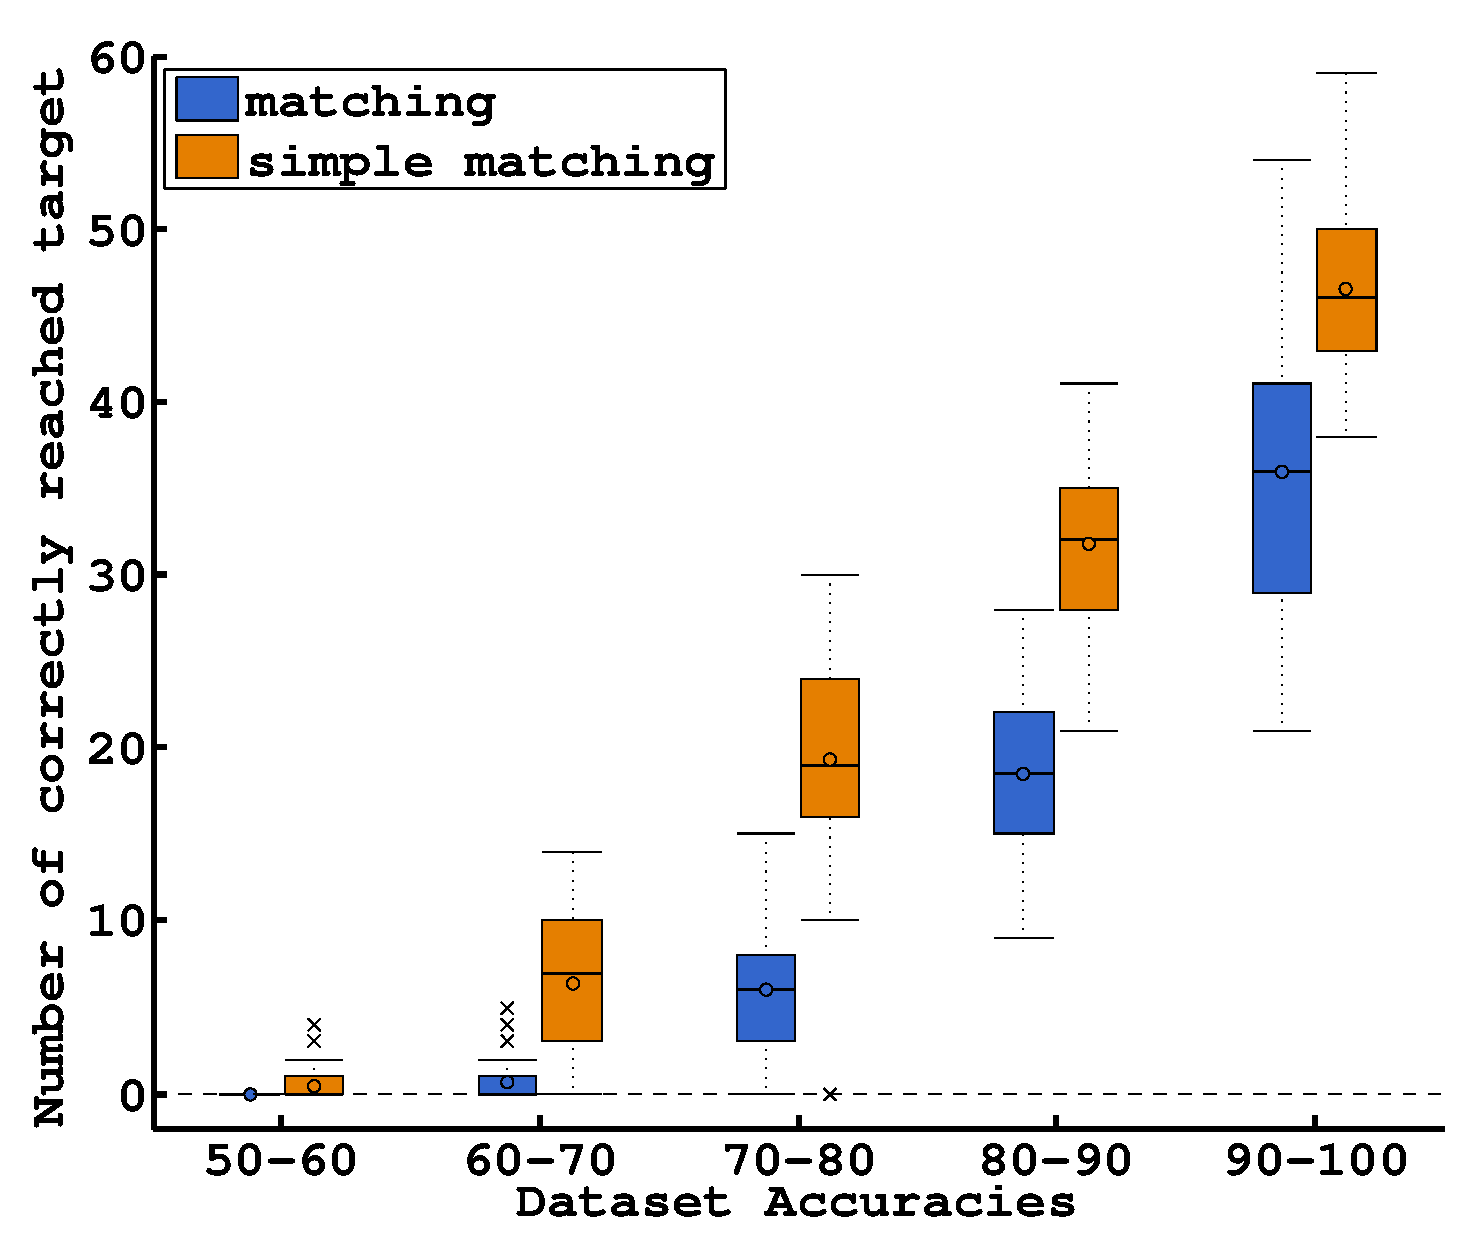
\includegraphics[width=\plotsize\columnwidth]{\imgpath/simplevsmatching/correct.eps}
\caption{Number of task correctly achieved in 500 steps with 2 dimensional artificial data. Comparison between Equation~\ref{eq:matchingfilter} (simple matching) and Equation~\ref{eq:matchingfiltercrossvalidation} (matching), where the latter correct the prediction of the classifier given the estimation of its confusion matrix. 
% The power information alone is sufficient to solve our problem but is less efficient than the other methods.
}
\label{fig:nCorrect_simplevsmatching}
\end{figure} 

\begin{figure}[!ht]
\centering
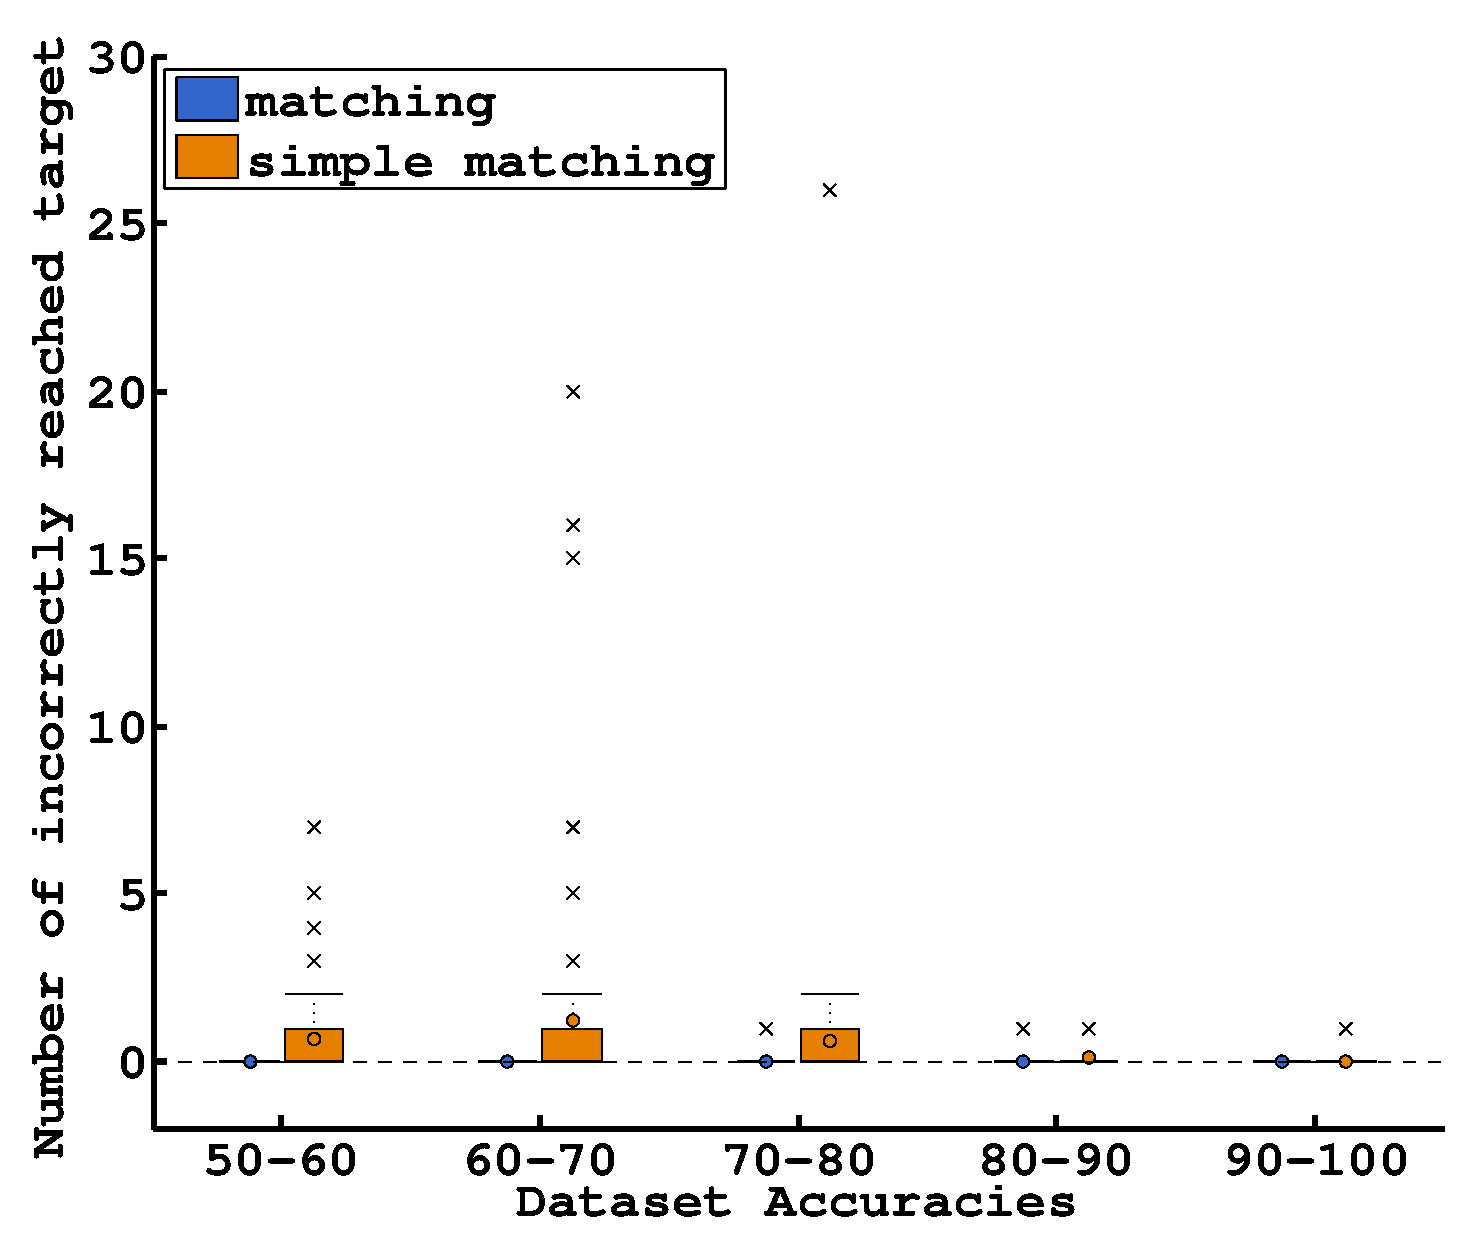
\includegraphics[width=\plotsize\columnwidth]{\imgpath/simplevsmatching/error.eps}
\caption{Number of task incorrectly achieved in 500 steps with 2 dimensional artificial data. Comparison between Equation~\ref{eq:matchingfilter} (simple matching) and Equation~\ref{eq:matchingfiltercrossvalidation} (matching), where the latter correct the prediction of the classifier given the estimation of its confusion matrix.
% The power information makes more mistakes for low quality dataset which also impact the power matching method. However those errors occurs for very low quality datasets, which are not the main targets of our algorithm.
}
\label{fig:nWrongEEG_simplevsmatching}
\end{figure} 


The power information alone is not enough to identify a high number of task, even if the number of steps to reach the first target are similar. The difference lies in the reallocation of labels we performed after a task is identified. As described in chapter~\ref{chapter:lfui:tasttotask}, once one task is identified with confidence we propagates its labels to all the other hypothesis. As a consequence, a majority of signal have identical labels, and the number of new signals with different labels needed to pull apart two hypothesis in terms of power ratio between classes increases. This is a problem resulting in measure relying only on global measure on the data. Our non-informed method (matching), measure the global quality of each classifiers but also consider the classification of each new signals individually, which speeds up the task reaching rate as the interaction goes on. See also the discussion of Figure~\ref{fig:sequence_evolution}.


Our results confirms that the use of the power information improves the performance of our algorithm. In addition, by disambiguating faster the task with symmetric properties, it also improves the visual impression our subjects get from the behavior of the agent with improved the quality of the signals received during our experimental test. At the time of writing those lines, this study was not over and this particular point requires a more detailed analysis to show and quantify this difference. It is particularly difficult to find a measure of perception of the agent behavior to quantify the difference between the use or not of the power information. We can only report here our experience from running the experiments, which is the reason of using the power information.


This is not possible with model method as the one presented in section~\ref{chapter:limitations:overlap}. Indeed to compute the prediction error of a model or a classifier, we need to compare its prediction with what is expected as a prediction. The labels outputted from our classifier can be compared with the label given in input. But for a model that output the probability of a particular signal, we can not compared the the true probabilistic value of each point and therefore we cannot quantify the prediction errors of such model.
%!TEX root = ../../thesis.tex

\section{Word properties}
\label{chapter:limitations:wordlproperties}


\question{How the world properties (symmetries, size, \ldots) affect the learning properties?}

As discussed in chapter~\ref{chapter:lfui:symmetries}, the properties of the world can affect the learning performances. For example some worlds have symmetric properties which makes some tasks impossible to differentiate. 

In this section, we compare how various planning method perform on our two different worlds, namely the pick and place scenario and the grid world. We will investigate a random strategy, several $\epsilon$-greedy (where the agent follows the best strategy or select an action randomly $\epsilon$ of the times), a strategy based on the task uncertainty (where we do not take the signal to meaning mapping uncertainty in to account), and our uncertainty based method described in chapter\ref{chapter:planning}. We will see that the size and the optimal policies properties of each world impacts the performances of some planning methods.

\subsection{Hypothesis and world properties}

Our hypothesis is that differences in size and optimal policies properties of each world will impacts the performances of some planning method considered, especially the random method which was performing quite well in our previous examples of chapters~\ref{chapter:planning}~and~\ref{chapter:bci}.

In the coming analysis we will consider three different world, a 5 by 5 grid world, a 25 by 25 grid world and our pick and place world of chapter~\ref{chapter:lfui}. In the following we present the main differences between those worlds.

First testing our planning method on a 5x5 and 25x25 allow to test how the size of the world influence the performance of each of the method and verify that our uncertainty measure is robust to such change. The main hypothesis is that the random action selection method will not scale well to this change in dimensionality. In a 5x5 grid, random actions allow to cover the space quite uniformly in 100 time steps, however in a 25x25 the robot will not succeed in exploring all the state and is therefore unlikely to visit useful states at every experiments.

We choose to use a 25x25 grid because the resulting number of state (625) is similar to the number of state of our pick and place scenario (624), which allow to remove the size effects when comparing those two scenarios. By comparing the grid world and the pick and place scenario, we aim at investing how the maze like properties of the pick and place word compares with the less strict properties of the grid world. For the pick and place scenario, to reach the correct cube configuration the robot must achieve a very specific sequence of action in the correct order. Like for going out of a maze, only one correct path can be followed. However for the grid world, a multitude of path can be chosen. 

This can be measure by the amount of overlap between the optimal policies associated to two ``close'' task. For the pick and place scenario, if the signal to meaning mapping were known, to differentiate between two cube configuration that are close together, the agent must go towards those configuration to be able to discard one or an other task. For example, in our illustration of Figure~\ref{fig:lfui:pickplacesequence}, to differentiate between the two first state, one as to reach one of those two states to tell the identify the correct one. Indeed, their corresponding optimal policies are similar for every state except their two final states, i.e. both tasks share the same policies for 622 states our of 624. However for the grid world scenario, if the signal to meaning mapping were known, one could differentiate between the top right state and the state directly on the left of that top right state by simply performing a left action on the bottom right state. And this whatever the size of the grid. The optimal policies of those two task differs for all states along the two columns on the left of the grid, i.e. both tasks share the same policies for only 575 states our of 625 in our 25x25 grid world.

\subsection{Method}

we use a feedback frame, and the method used in planning for all our updates rule.

50 run each method each world
90-100 percent datasets

\subsection{World size effects}


\todo{figure to compare 5x5 and 25x25}

\todo{important say that we are optimistic in the plot, saying that if they do not reach, we count 100, which is actualy optimistic}


\subsection{Maze properties effects}

\begin{figure}[!ht]
\centering
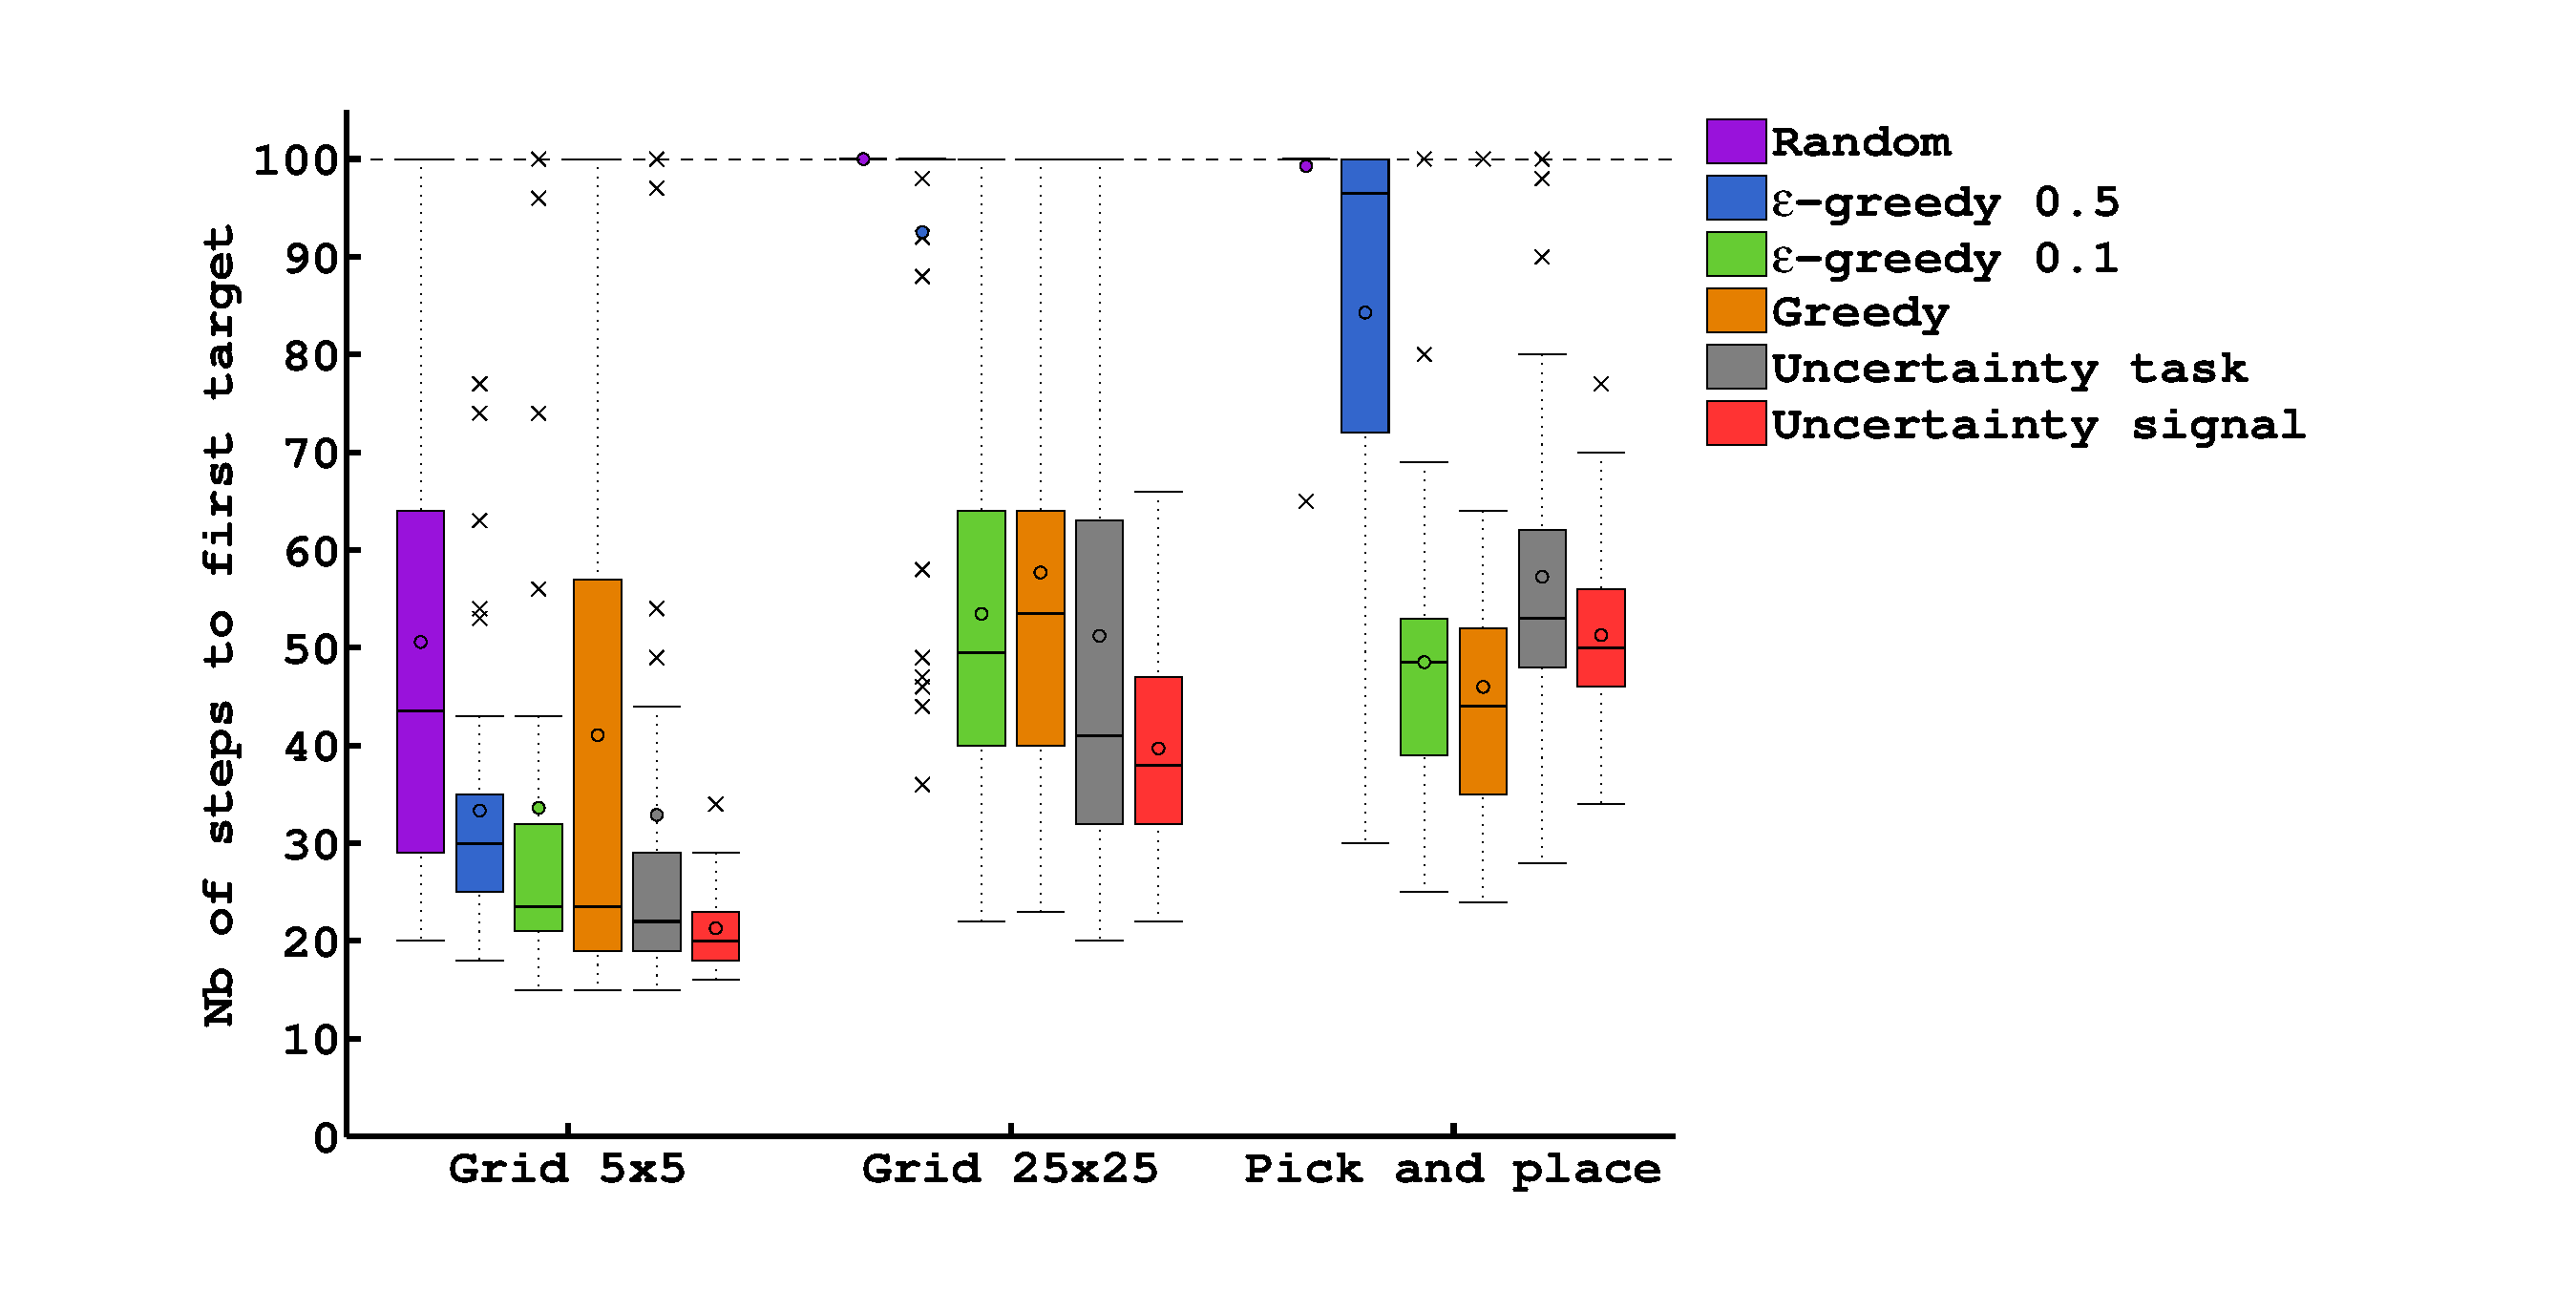
\includegraphics[width=\legendsidesize\columnwidth]{\imgpath/world_properties/firstreach.eps}
\caption{Number of steps to reach first target state with confidence.}
\label{fig:wordlpropertiestimefirst}
\end{figure}

We report only 9 erroneous first task estimations across all runs of our experiments and conditions.For the grid world, 1 error for the Greedy method in. For the pick and place scenario, 1 for $\epsilon$-greedy 0.5, 2 for $\epsilon$-greedy 0.1, 2 for Greedy, 1 for Uncertainty task and 2 for Uncertainty signal.

\begin{table}[!ht]
\centering
\rowcolors{2}{gray!25}{white}
\begin{tabular}{c c c c}
    Planning method & Gridworld 25x25 &  Pick and place \\ \hline
    Random & 0 & 1 \\ 
    $\epsilon$-greedy 0.5 & 13 & 27 \\
    $\epsilon$-greedy 0.1 & 48 & 48 \\
    Greedy & 43 & 47 \\
    Uncertainty task & 42 & 48 \\
    Uncertainty signal & 50 & 50 \\
\end{tabular}
\caption{Number of experiments that reached at least one target in 100 steps.}
\label{tab:}
\end{table}

\begin{figure}[!ht]
\centering
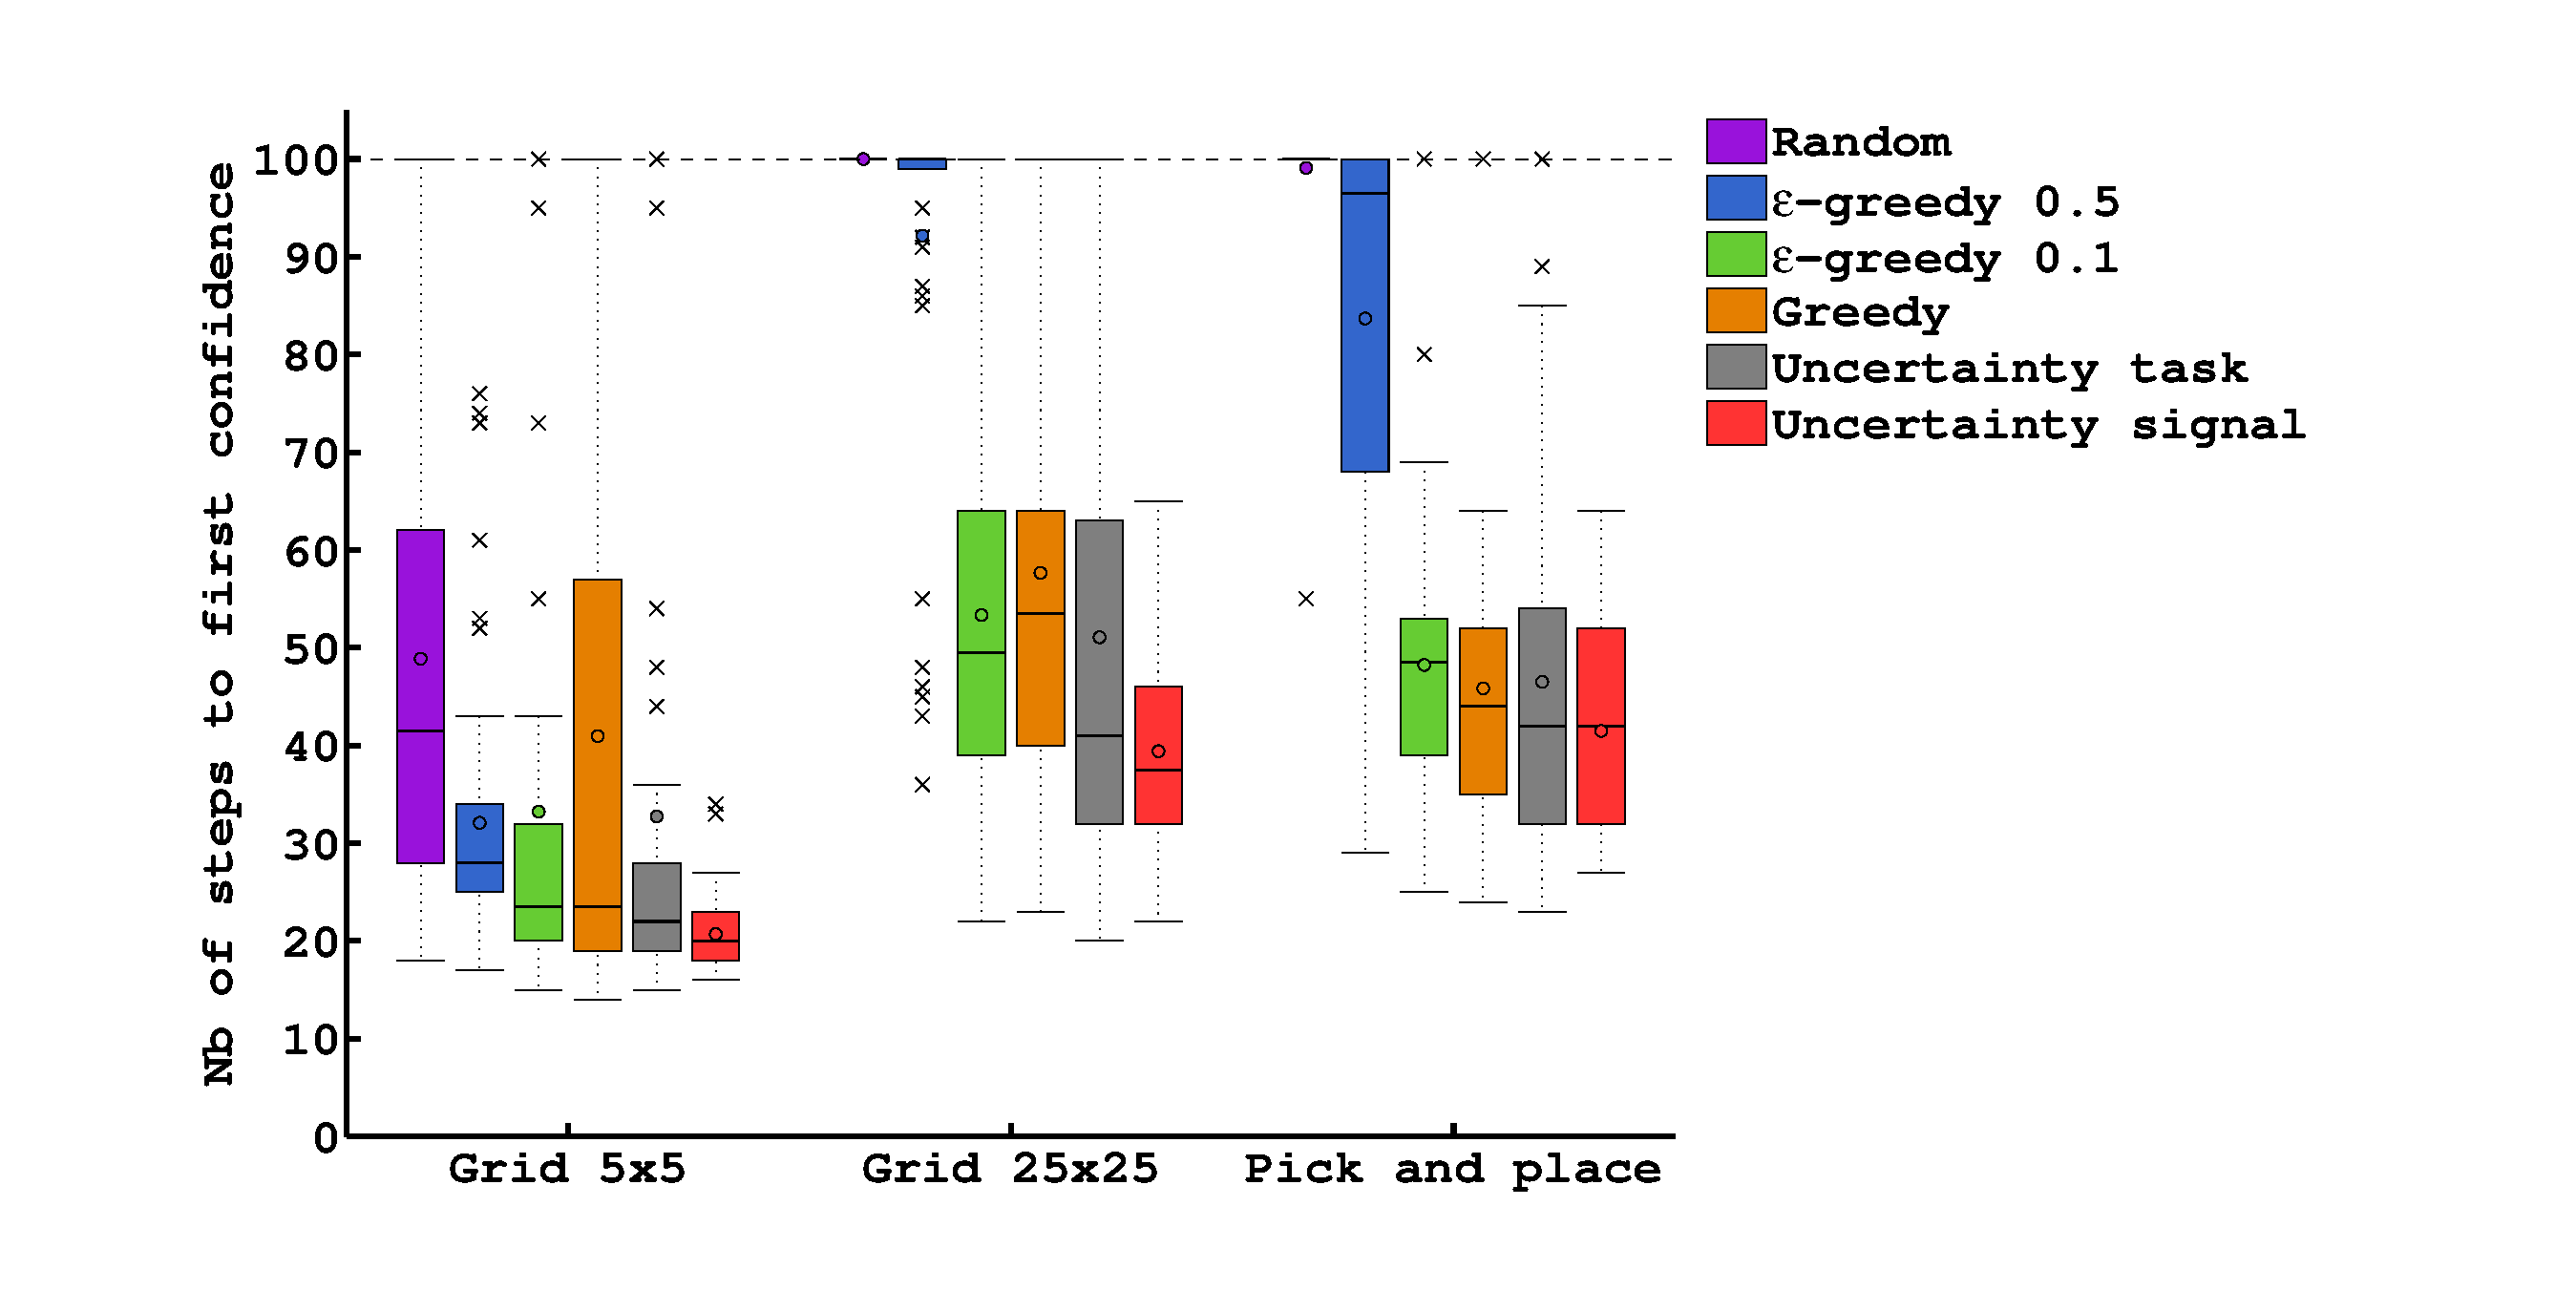
\includegraphics[width=\legendsidesize\columnwidth]{\imgpath/world_properties/firstconfident.eps}
\caption{Number of steps to reach confidence level for the first target.}
\label{fig:wordlpropertiesconfidencefirst}
\end{figure} 

\begin{figure}[!ht]
\centering
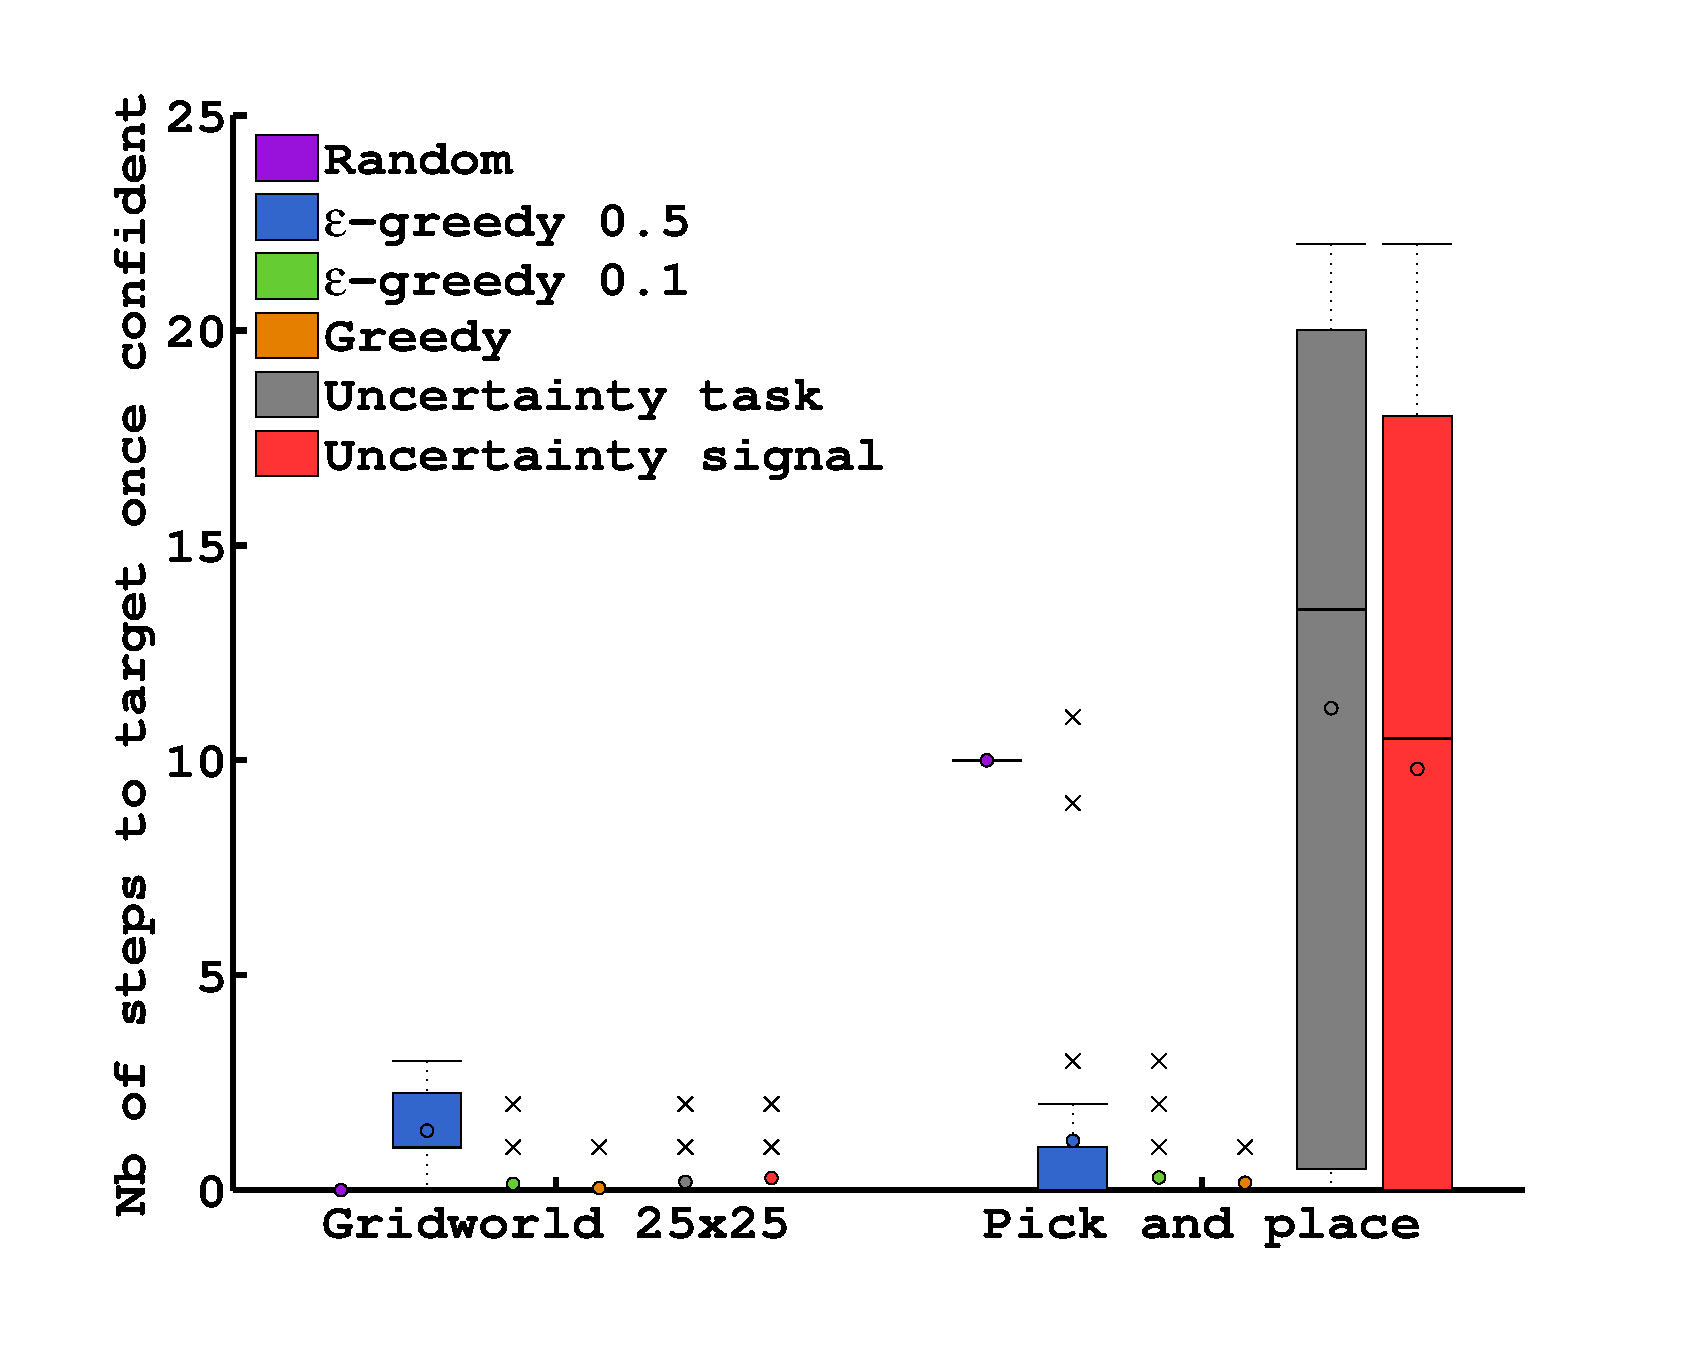
\includegraphics[width=\plotsize\columnwidth]{\imgpath/world_properties/difftargetconfidence.eps}
\caption{Number of action needed to reach the first target when the agent reach confidence level for this target.}
\label{fig:wordlpropertiestargetdist}
\end{figure} 

refer to experiment with pick and place in section lfui and random planning (even if dataset the same after 100 step no confidence) but state space is 625 and no ore 25...
random after 100 not at the confident level.


\subsection{Discussion}

it is obviously dependent on plenty of other things not tested here the frame and signals quality and stuff

should we compare on the number of state or on the number of state action pair?

conclude by stating difference between end goal learning (graps object, reach state) and reward based learning. We only consider goal learning. episodic (find the right box) vs endless (collect more reward), different exploration function could be used for those


%!TEX root = ../../thesis.tex

\section{Exploiting overlap between distributions}
\label{chapter:limitations:overlap}


In this section, we propose a method that uses the overlap between the model for each class to identify the correct task hypothesis, and demonstrate the efficiency of our uncertainty measure on the signal space presented in chapter~\ref{chapter:planning:uncertaintysignalspace}. We present simulated experiments using pre-recorded EEG signals, and show that we achieve similar performances than calibration based systems. Finally, we report online experiments where four users control, by means of a BCI, an agent on a virtual world to reach a target without any previous calibration process.

\subsection{Using the Bhattacharyya coefficient}

Following \cite{blankertz2010single}, we model the EEG signals using independent multivariate normal distributions for each class ($\mathcal{N}(\mu_c, \Sigma_c)$ and $\mathcal{N}(\mu_w, \Sigma_w)$). We will denote by $\theta$ this set of parameters $\{\mu_c, \Sigma_c,\mu_w, \Sigma_w\}$.

We propose to exploit the fact that when labels are mixed, the Gaussian corresponding to each classes should overlap more than for the correct label association (see Figure~\ref{fig:TworldLabelGaussian}). The Bhattacharyya coefficient measures this overlap, it has been related to the classification error of Gaussian models \cite{Kailath67} and is inversely proportional to the classification rate. Although there is no analytical relation between the coefficient and the classification rate, it is possible to derive bounds and good empirical approximations \cite{lee2000bayes}.

The Bhattacharyya coefficient $\rho \in [0,1]$ between the Gaussian distributions associated to label ``correct'' ($\mathcal{N}(\mu_c, \Sigma_c)$) and ``incorrect'' ($\mathcal{N}(\mu_w, \Sigma_w)$) is:

\begin{eqnarray}
\rho = e^{-D_B(\theta)}
\end{eqnarray}

where $D_B$ is the Bhattacharyya distance:

\begin{eqnarray}
D_B(\theta) = \frac{1}{8}(\mu_c-\mu_w)^T(\frac{\Sigma_c+\Sigma_w}{2})^{-1}(\mu_c-\mu_w)+\frac{1}{2}ln\left(\frac{det(\frac{\Sigma_c+\Sigma_w}{2})}{\sqrt{det\Sigma_c det\Sigma_w}}\right)
\end{eqnarray}

Finally, we approximate the expected classification rate as:
\begin{eqnarray}
Ecr \propto 1 - \rho
\end{eqnarray}

Now that we have an estimation of the expected classification rate, which is proportional to the overlap between the model of each class, we need to take a decision with respect to which task is the one intended by the user. To do so we compare the expected classification rate of every task hypothesis $\xi_t$ with $t \in \{1, \ldots, T\}$. 

The hypothesis whose associated model overlaps the less, i.e. which has the highest expected classification rate, i.e.\ the lowest value of $\rho$, is expected to be the one intended by the user. However it is meaningless to define an absolute threshold on the value of the expected classification rate itself. Indeed, different people generate different signals which result in classifiers of different qualities. Also, even the for the correct signal-label pairs, the model may overlap by quite some amount, as shown in our 2 dimensional examples in Figure~\ref{fig:datasetsquality}. To bypass this problem we rely on a voting system where we attribute to each hypothesis $\xi_t$ a weight that is updated at every iteration.

We rely on a pseudo-likelihood metric that for each hypothesis $\xi_t$ accumulates the expected classification rate over time:

\begin{eqnarray}
\L(\xi_t) = \prod_{i = 1}^{M} 1 - \rho_i^{\xi_t}
\end{eqnarray}
%
with $M$ the current number of iteration and $\rho_i^{\xi_t}$ the Bhattacharyya coefficient associated to task $\xi_t$ using all data up to time $i$. By normalizing the pseudo-likelihood values between every hypothesis, we obtain what can be viewed as the probability of each target:

\begin{eqnarray}
p(\xi_t) = \frac{\L(\xi_t)}{\sum_{u \in \{1, \ldots, T\}} \L(\xi_u)}
\end{eqnarray}

Once a target reaches a probability threshold $\beta$ we consider it as being the correct one, i.e.\ the one intended by the user. We used $\beta = 0.99$.

Finally, once we identified the first target, we will switch back to a classification based algorithm as described in chapter~\ref{chapter:lfui:tasttotask} and as used in the previous chapters of this thesis. We will see in section~\ref{chapter:limitations:overlap:offline} that this switch is necessary to maintain good performances since the classifier makes a much harder decision for each new EEG signal.

\subsection{Planning}

As we are using a model based method, we rely on our method measure that measure uncertainty directly in the signal space. This method was described in chapter~\ref{chapter:planning:uncertaintysignalspace} and to summarize rely on computing, for every state-action pairs, the similarity between the expected signals for each task. The more the expected signals are similar the less there is uncertainty.

For computing the similarity between two Gaussian distributions we could rely again on the Bhattacharyya coefficient describe above. However computing this coefficient between all models and for all state-action pairs was not feasible in real time. In order to improve computation efficiency we do not rely on a precise metric between Gaussian distributions and only consider the similarity between their means. The closest the means are, the more similar they are.

\subsection{Offline analysis}
\label{chapter:limitations:overlap:offline}

The objective of the offline analysis is to study the impact of our exploration method and evaluate if the classifier learned from scratch with our algorithm can be reused for learning new tasks. To ensure we have sufficient data to achieve statistically significant results, we rely on a large dataset of real EEG data. We used the same dataset as describe in chapter~\ref{chapter:bci:EEGsignals} dataset from \cite{iturrate2013task}, which covers ten subjects that performed two different control problems.

For each subject, we simulated 20 runs of 400 iterations following the control task. Each time the device performed an action, we sampled the dataset using the ground truth labels corresponding to the correct task and then removed the chosen signal from it. After a first task was identified we continued running the system to identify new tasks. 

We present most of the results in terms of the quality of the dataset, measured as the classification accuracy that a calibrated brain signal classifier would obtain.

\paragraph{Planning Methods}

We compared the average number of steps (with maximum values of 400 steps) needed to identify the first task when learning from scratch with different planning methods.

\begin{figure}[!htbp]
    \centering
    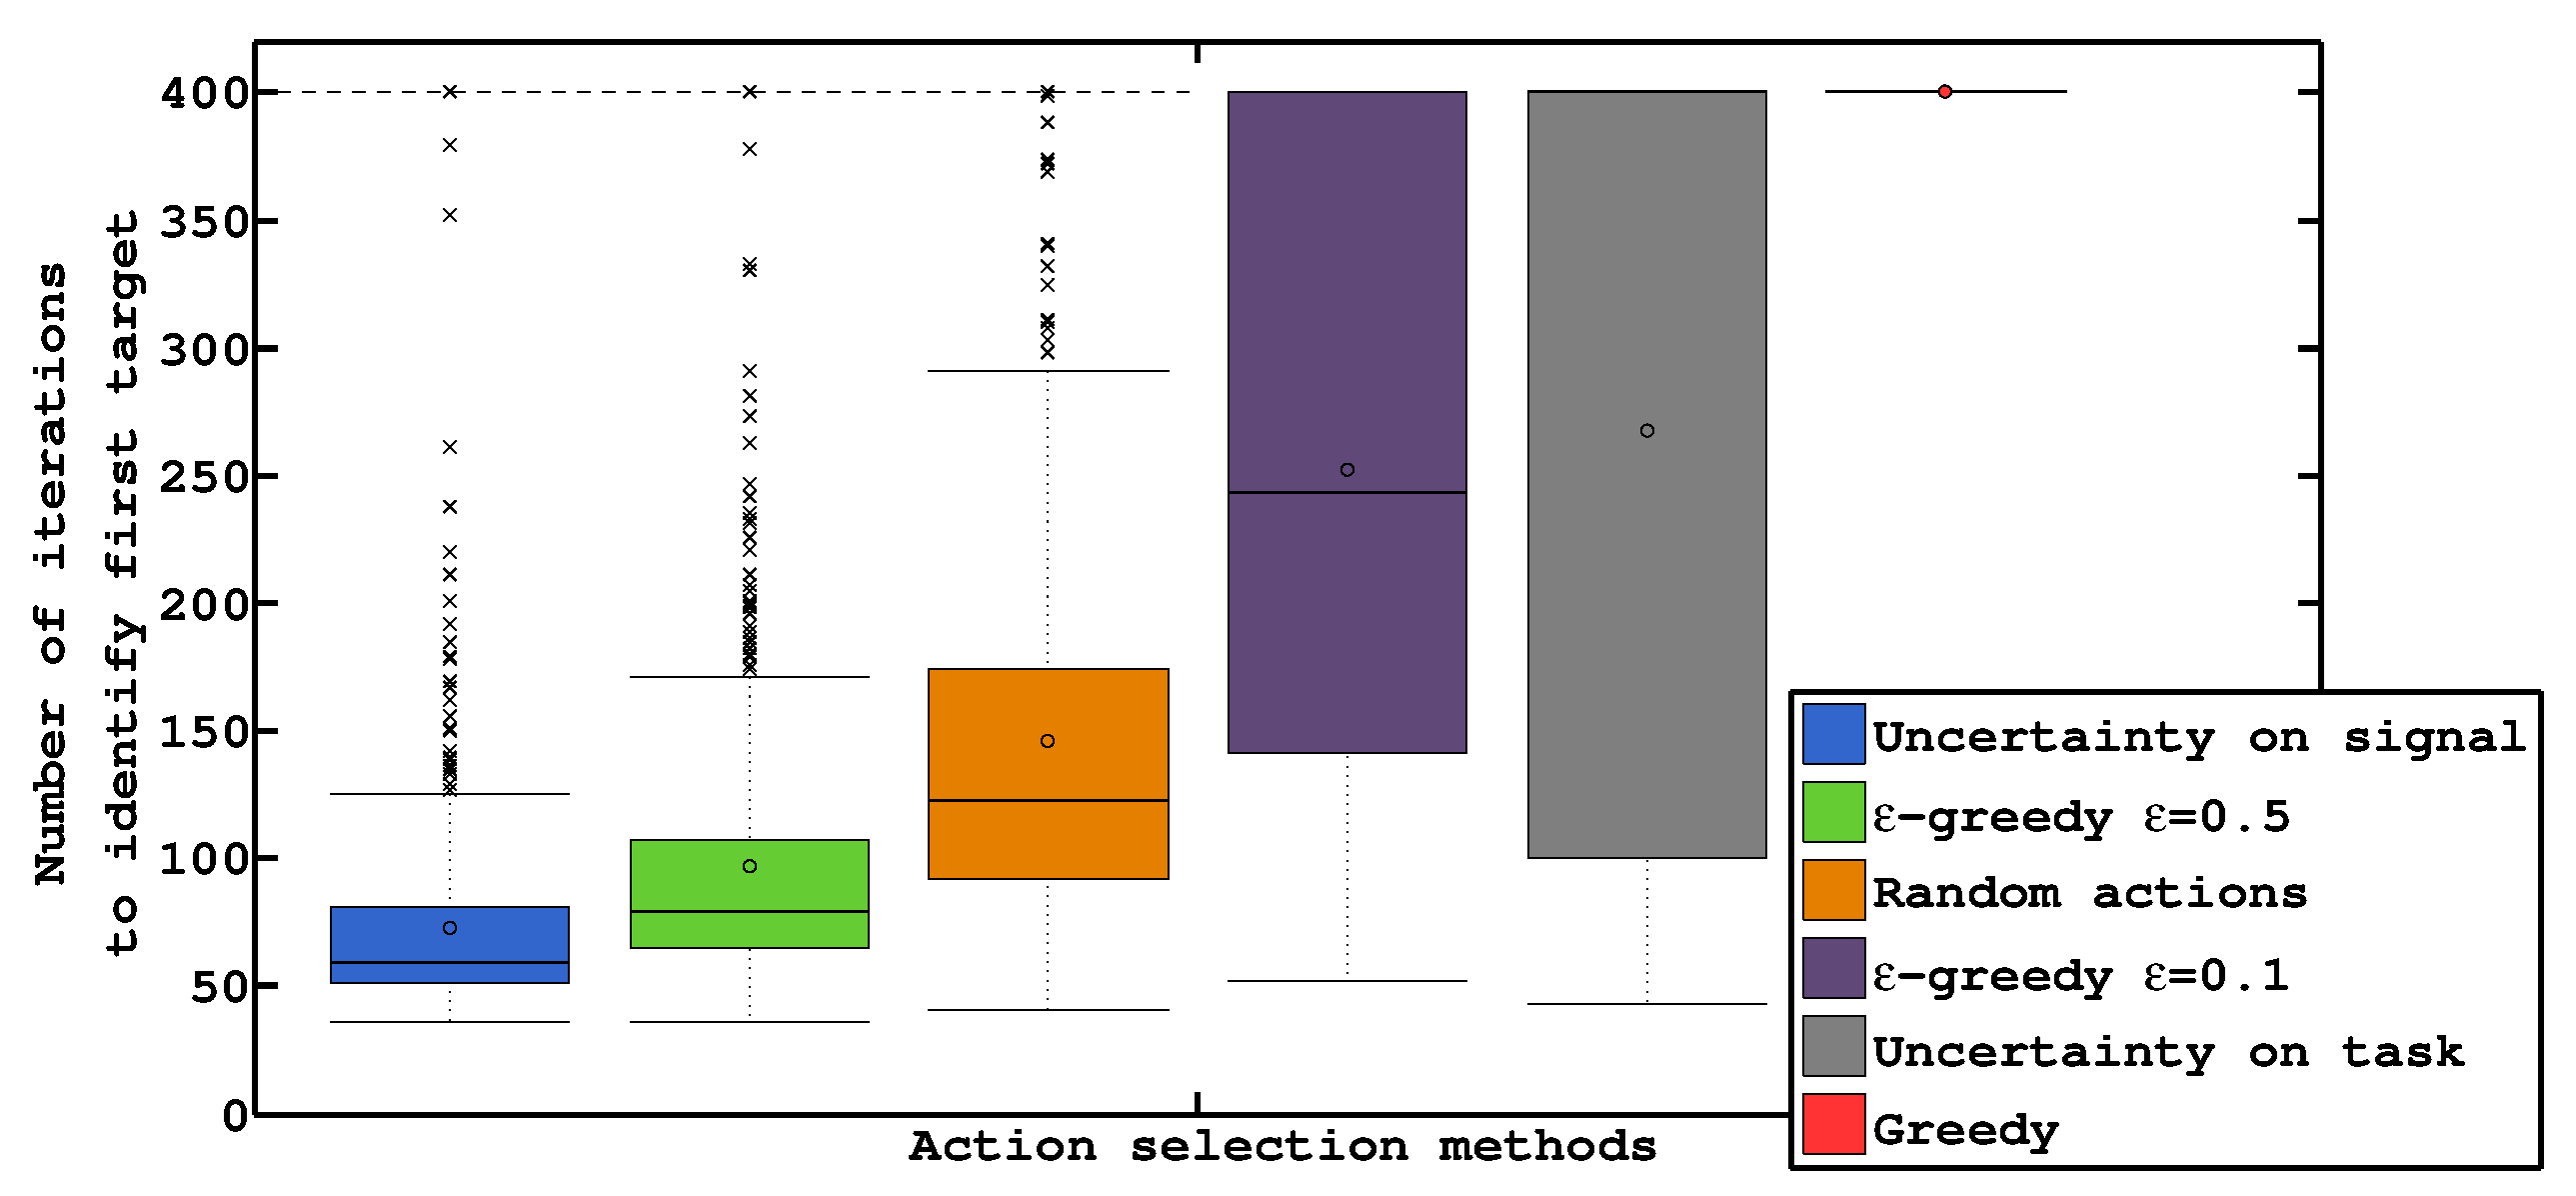
\includegraphics[width=\columnwidth]{\imgpath/battacharyya/plot_planning_first.eps}
    \caption{Comparison of different exploration methods. Our proposed method, based on the uncertainty on the expected signal, allows to lead the system to regions that improve disambiguation among hypotheses in a faster way. For the greedy method, all values were 400 which indicates it never allowed to identify any task.}
    \label{fig:overlapcompplan}
\end{figure}

Figure~\ref{fig:overlapcompplan} shows the results averaged across subjects, runs and datasets. Values of 400 means the confidence threshold was not reached after 400 iterations. Our proposed method, based on the uncertainty on the expected signal, allows to lead the system to regions that improve disambiguation among hypotheses in a faster way. Trying to follow the most probable task does not allow the system to explore sufficiently (Greedy), and at least some random exploration is necessary to allow a correct identification of the task ($\epsilon$-greedy). Assessing uncertainty only on the task performs poorly as it does not take into account the signal interpretation ambiguity inherent to our problem. The large variability in the results is mainly due to the large variations in classification accuracy across subjects and datasets. Given these results, the remainder of this section will only consider our proposed planning method.

\paragraph{Using the Bhattacharyya coefficient in the long run}

After identifying the first task, and following our approach, we continued running the system and measured how many tasks were identified after 400 steps. Figure~\ref{fig:overlapbhatta} demonstrates the advantage of switching to a classification based method after identification of a first target instead of keeping the estimation given by the Bhattacharyya coefficient. On the one hand, Bhattacharyya coefficient works very well for small amounts of data because it directly compares model parameters. On the other hand, after identifying many task, all models share most of their signal-label pairs and it requires much more data to modify the models and detect overlaps. Therefore using a classifier allows for a faster identification since the classifier makes a much harder decision for each new EEG signal. This discussion is in line with the observation on the use of the power information made in chapter~\ref{chapter:bci:priorpower}.

\begin{figure}[!htbp]
    \centering
        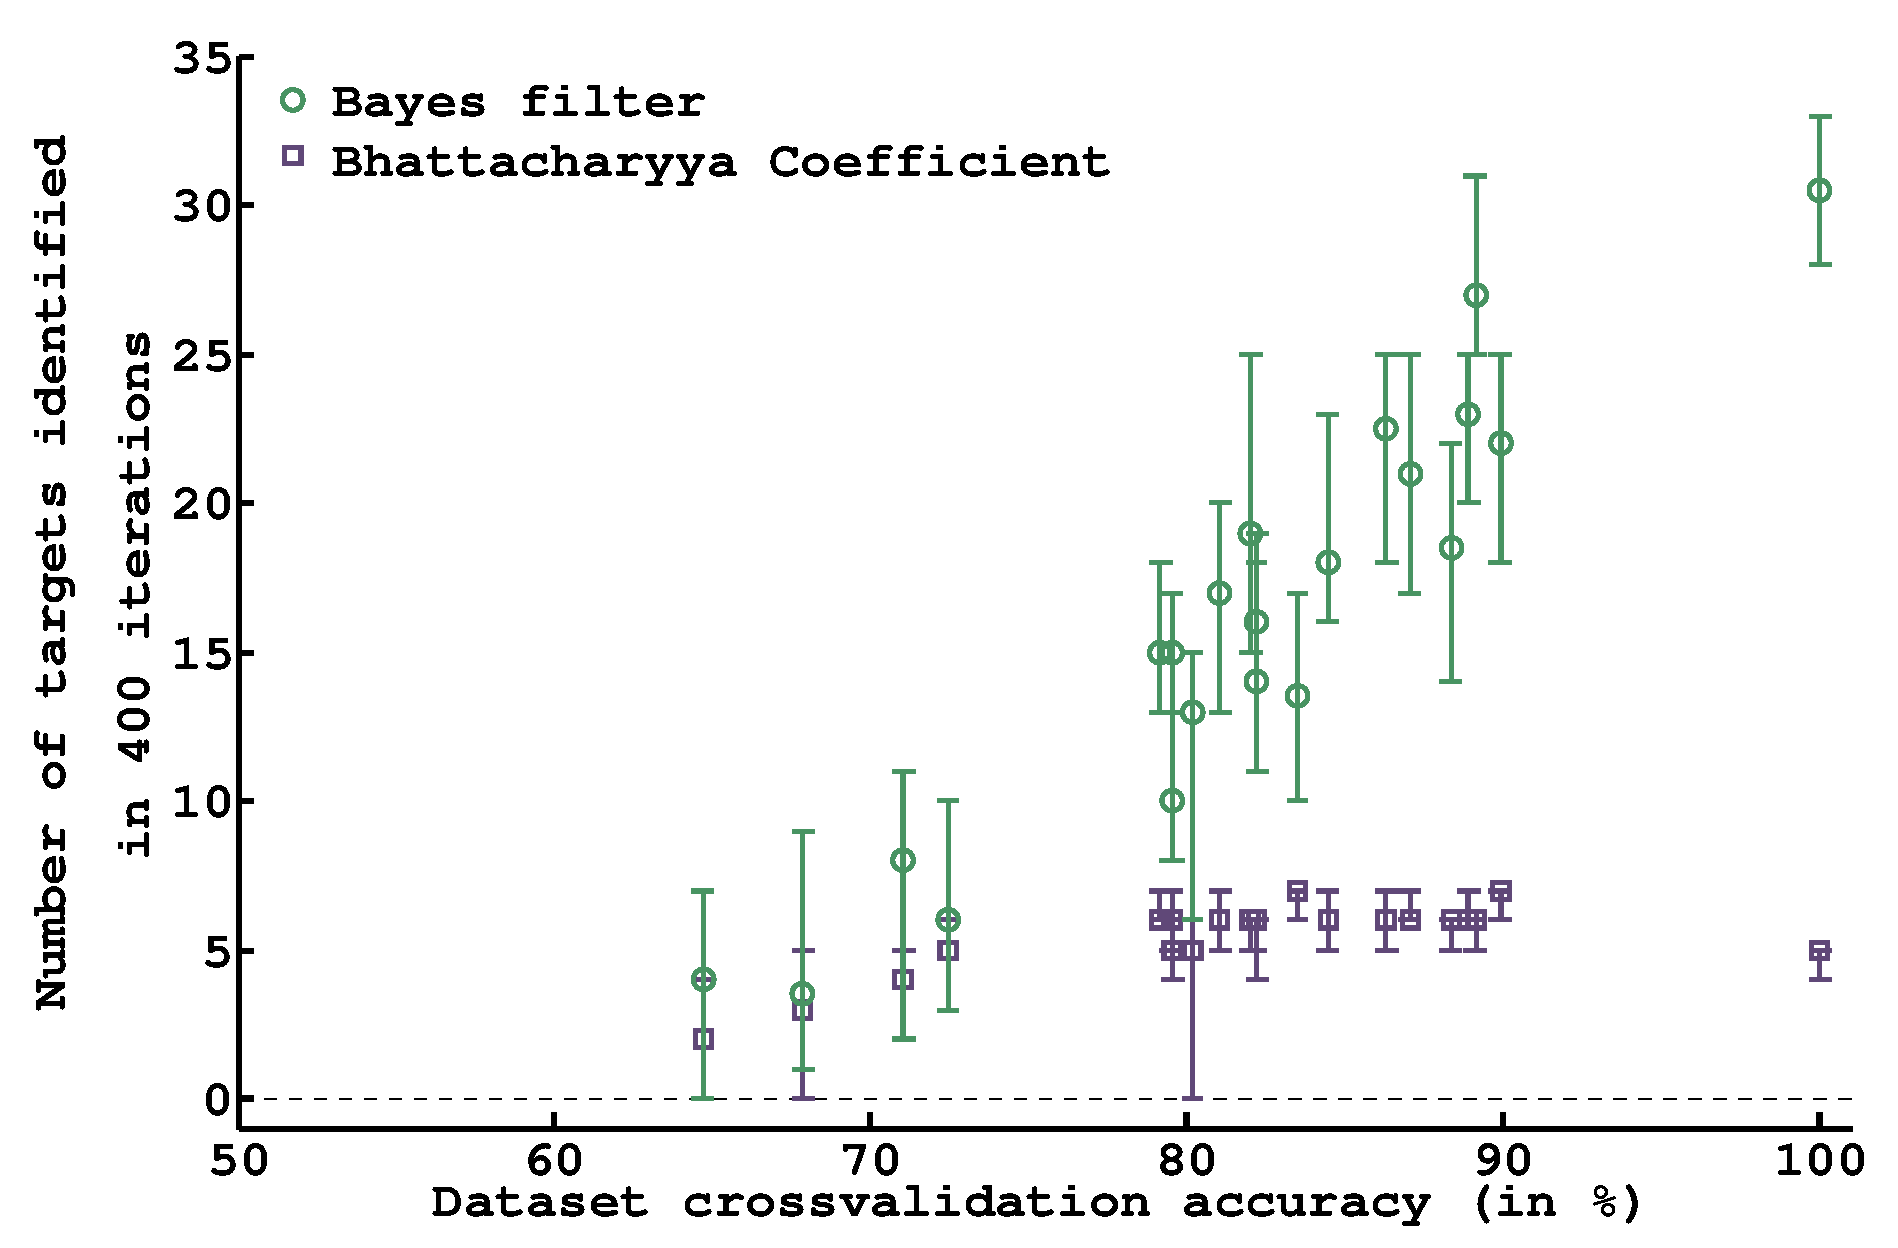
\includegraphics[width=\plotsize\columnwidth]{\imgpath/battacharyya/plot_bhattha_vs_bayes}
        \caption{Number of targets correctly identified in 400 iterations (the markers show the median values and the error bars the 2.5th and 97.5th percentiles). Comparison between switching to a Bayes filter method after identification of a first target instead of keeping the estimation given by the Bhattacharyya coefficient. The classification based method allows for a faster identification.}
        \label{fig:overlapbhatta}
\end{figure} 

Given these results, in the remaining of this section we only consider switching to a classification based method once the first task has been identified.

\paragraph{After 400 steps}

Figure~\ref{fig:overlapavg_sum_400} shows the number of tasks correctly and incorrectly identified in 400 iterations. For datasets of good qualities, we are able to identify more than 20 tasks in 400 iterations without the need for a calibration procedure (recap that previous works needed between 300 and 600 examples for the calibration phase \cite{chavarriaga2010learning,iturrate2010single}). The number of correctly identified tasks is strongly correlated to the quality of the dataset.

\begin{figure}[!htbp]
    \centering
    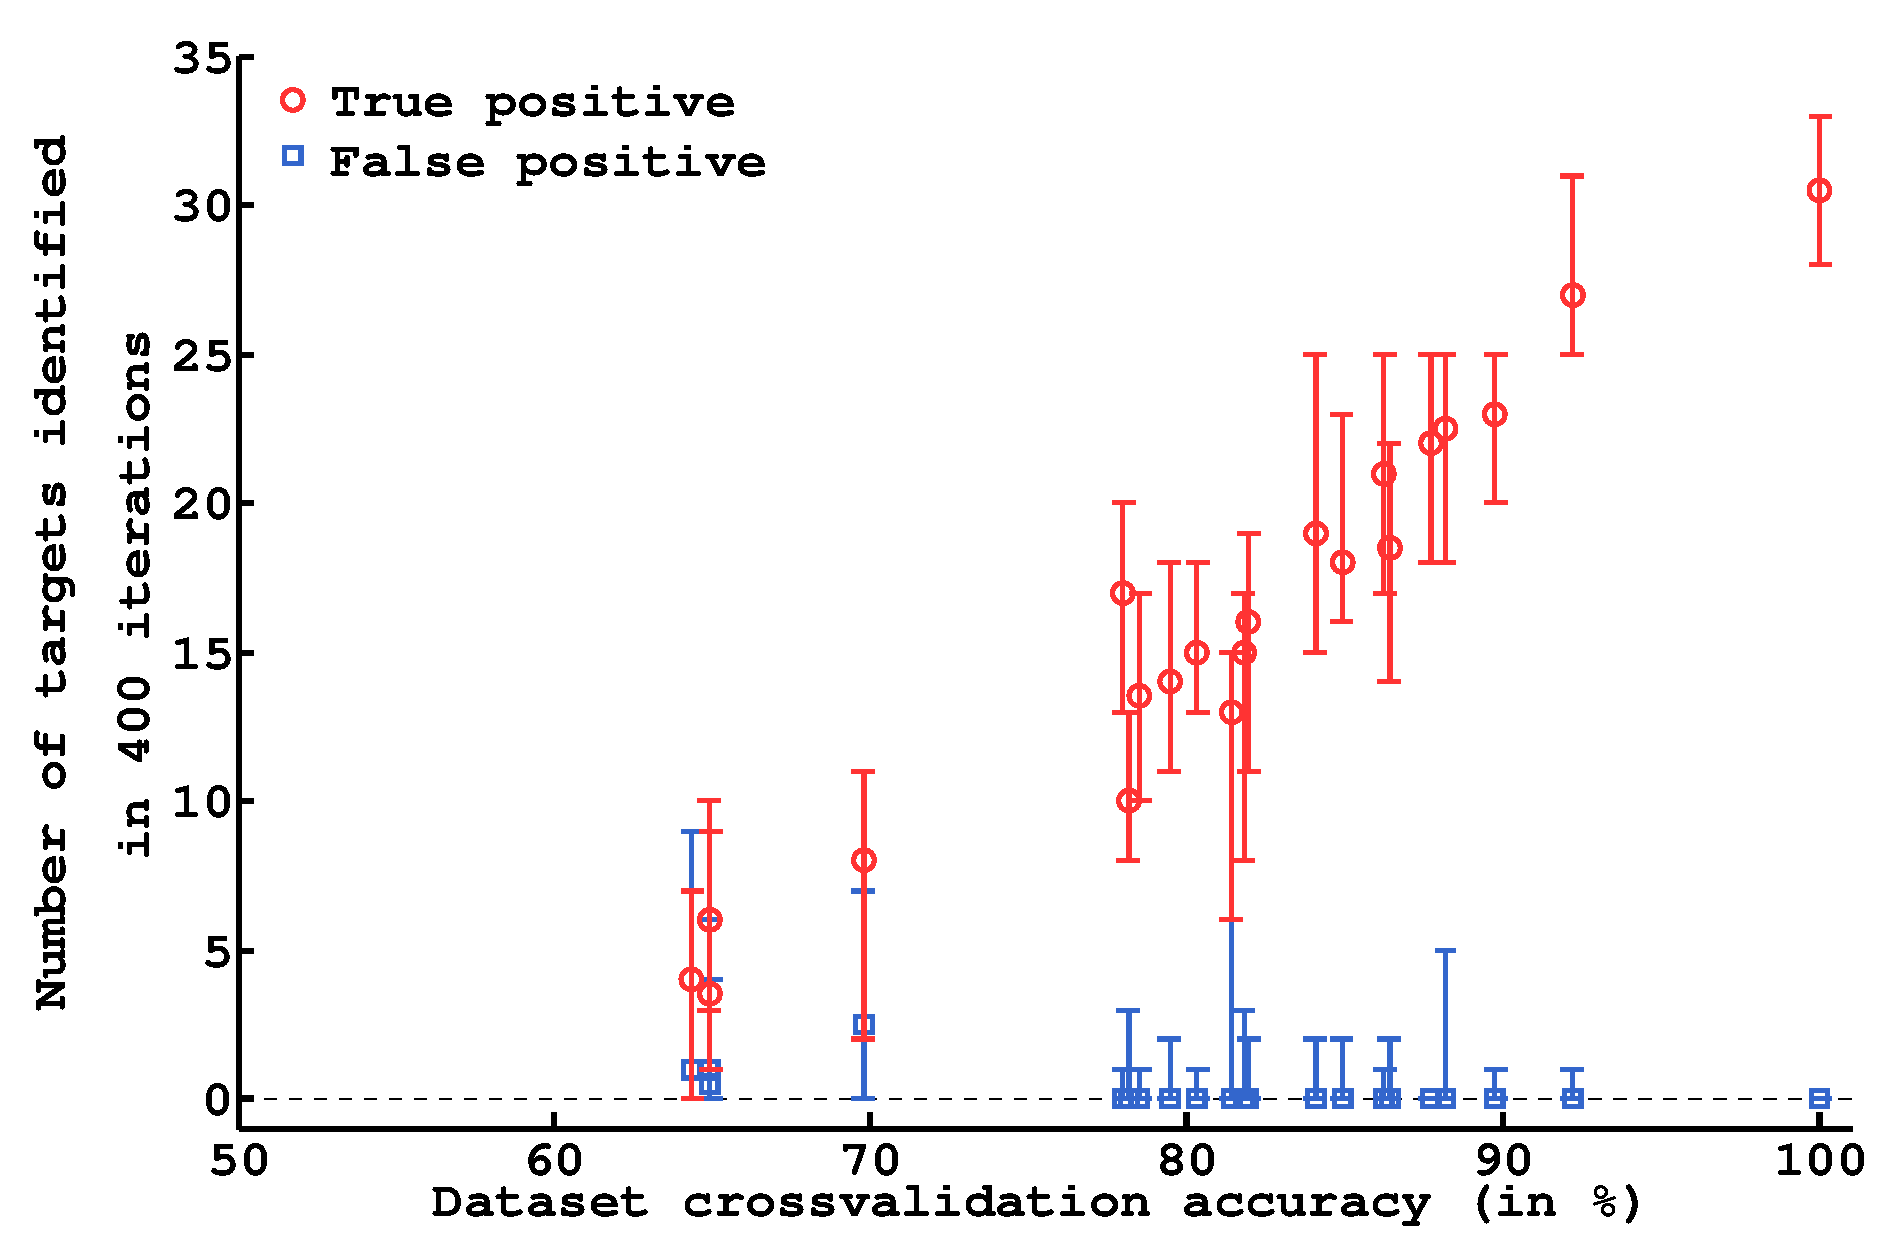
\includegraphics[width=\plotsize\columnwidth]{\imgpath/battacharyya/plot_first400_reach} 
    \caption{Number of targets correctly and incorrectly identified in 400 iterations (the markers show the median values and the error bars the 2.5th and 97.5th percentiles). For datasets of good qualities, we are able to identify more than 20 tasks in 400 iterations without the need for a calibration procedure.}
    \label{fig:overlapavg_sum_400}
\end{figure} 

The quality of our unsupervised method can be measured according to the percentage of labels correctly assigned (according to the ground truth label), see Figure~\ref{fig:overlappercentageLabels}. In general, having dataset with classification accuracies higher than 75$\%$ guaranteed that more than 90$\%$ of the labels were correctly assigned. This result shows that our algorithm can also be used to collect training data for calibrating any other state-of-the-art error-related potentials classifier, but has the important advantage of controlling the device at the same time.

\begin{figure}[!htbp]
    \centering
        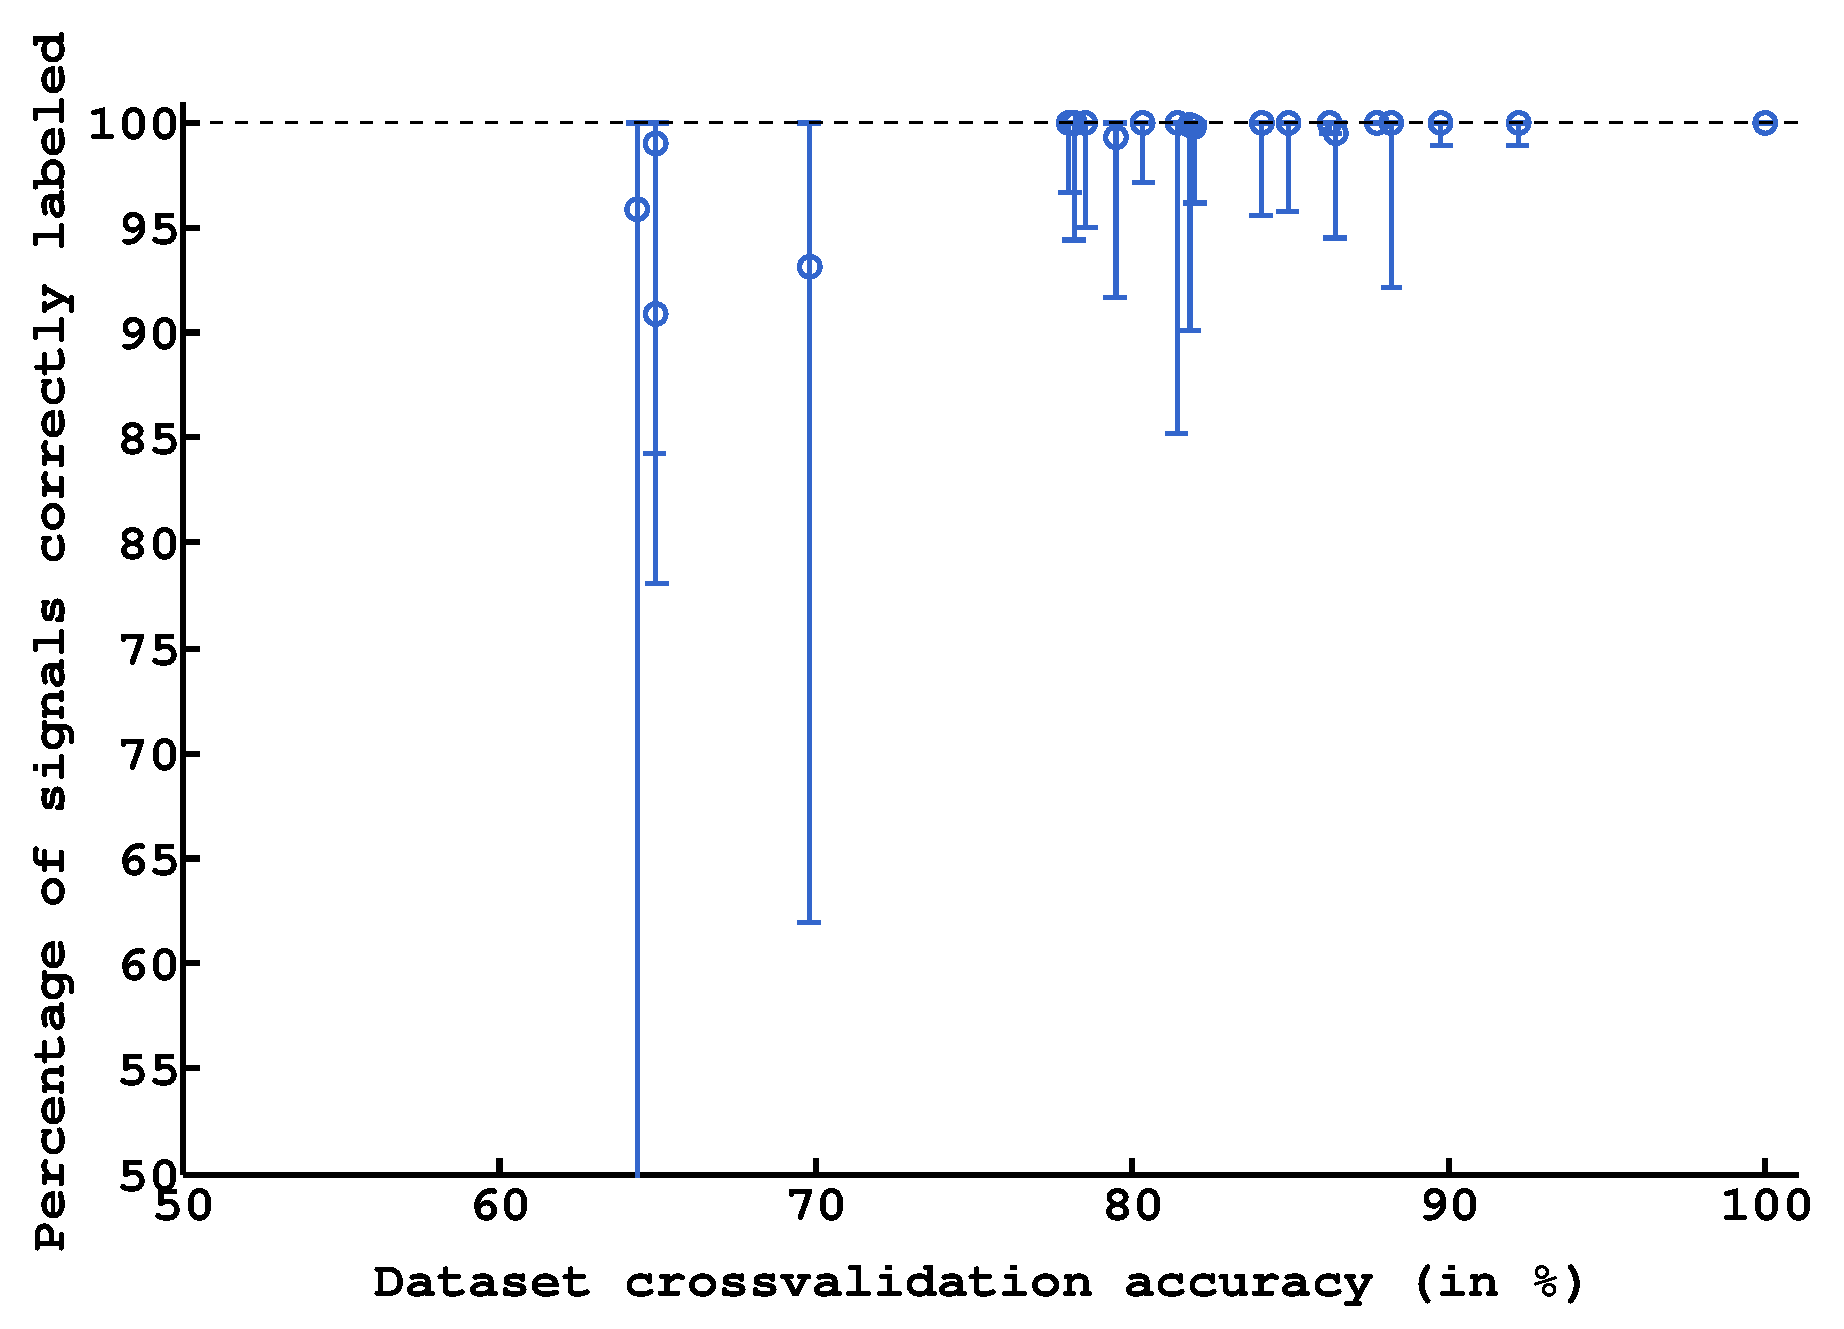
\includegraphics[width=\plotsize\columnwidth]{\imgpath/battacharyya/plot_percent_label}
        \caption{Percentage of labels correctly assigned according to the ground truth label (the markers show the median values and the error bars the 2.5th and 97.5th percentiles). In general, having dataset with classification accuracies higher than 75$\%$ guaranteed that more than 90$\%$ of the labels were correctly assigned.}
        \label{fig:overlappercentageLabels}
\end{figure}

\subsection{Online control}

The experiments were conducted with four subjects (aged between 25 and 28). Each subject was asked to mentally assess the agent's actions with respect to a given target. The system was not calibrated to decode the user EEG signals beforehand. Each subject performed 5 runs, for each run a new target was randomly selected and provided to the user. There was an action every three seconds. Each run lasted 200 actions, and the time between runs was around one minute.

The algorithm was able to identify the correct target for all runs of all the subjects, see Figure~\ref{fig:overlaponlineresults}. There are strong variations among subjects but we note that our system identified each task in less iterations than a normal calibration phase requires (between 300 and 600 examples depending on the user performance \cite{chavarriaga2010learning,iturrate2010single}).

\begin{figure}[!htbp]
    \centering
    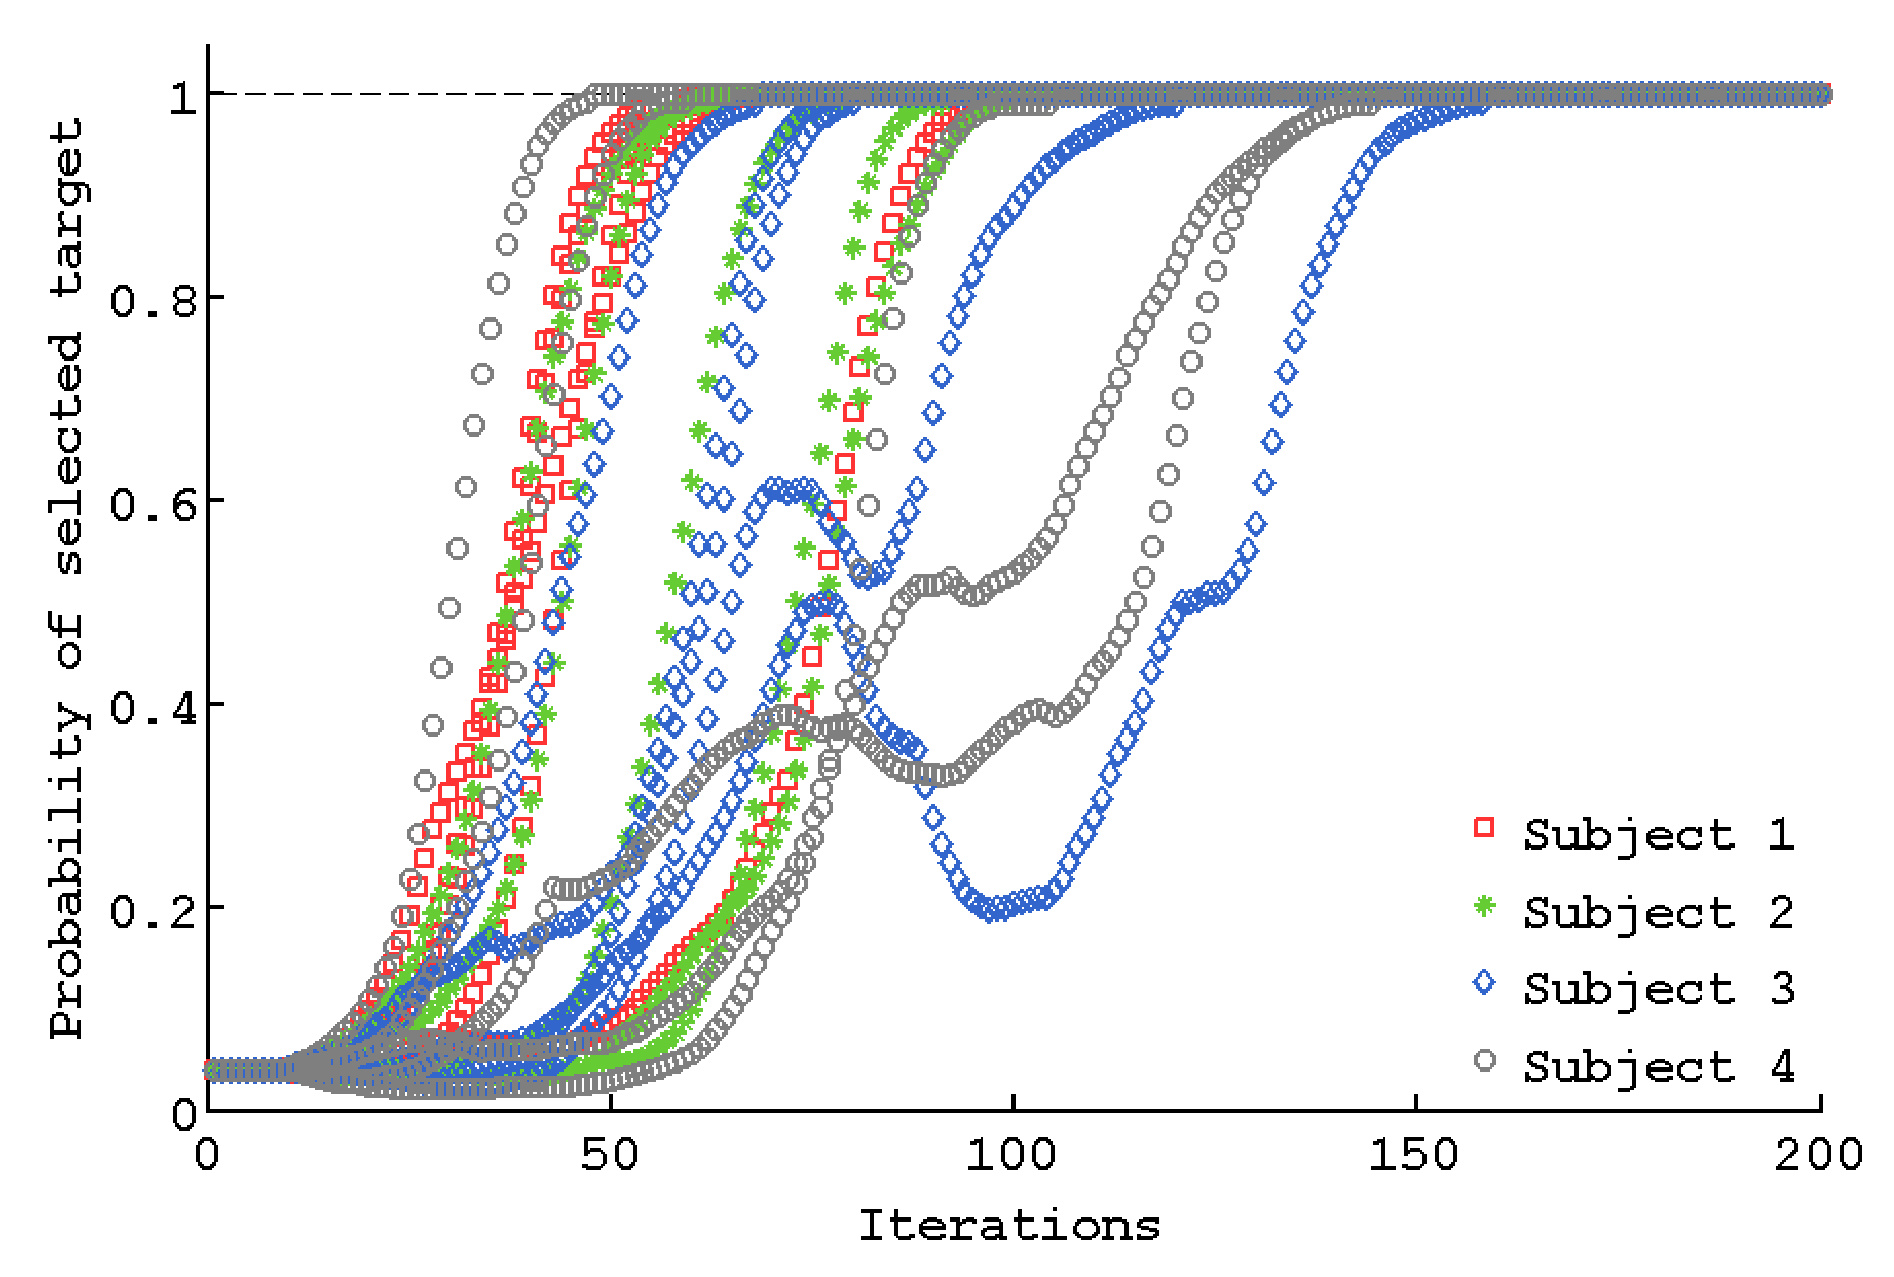
\includegraphics[width=\plotsize\columnwidth]{\imgpath/battacharyya/plot_realevolution}    
    \caption{Results from the online experiments: Evolution of the probability of the correct task for each subject and run. The algorithm was able to identify the correct target for each subjects and runs in less than 200 iterations.}
    \label{fig:overlaponlineresults} 
\end{figure}

Table~\ref{tab:overlaponline} shows for each subject and run the number of iterations needed to reach the confidence threshold for the subject selected target.

On average, the number of iterations needed to identify the target was of 85 $\pm$ 32.

\begin{table}[!htbp]
\centering
\rowcolors{2}{gray!25}{white}
\begin{footnotesize}
\begin{tabular}{r|rrrrr|r}
    %\toprule
    & \textbf{Run1} & \textbf{Run2} & \textbf{Run3} & \textbf{Run4} & \textbf{Run5} & \textbf{mean$\pm$std} \\\hline
    %\midrule
    \textbf{S1} & 95 & 62 & 56 & 60 & 64 & 67 $\pm$ 16 \\
    \textbf{S2} & 89 & 77 & 98 & 60 & 62  & 77 $\pm$ 17 \\
    \textbf{S3} & 68 & 80 & 118 & 76 & 157 & 100 $\pm$ 37 \\
    \textbf{S4} & 98 & 142 & 57 & 142 & 47 & 97 $\pm$ 45 \\
\end{tabular}
\end{footnotesize}
  \caption{Results from the online experiments: Number of iterations needed to identify the correct target for each subject and run. On average, the number of iterations needed to identify the target was of 85 $\pm$ 32.}
  \label{tab:overlaponline}
\end{table}

\subsection{Discussion}

We introduced a new method to exploit the facts that, when associated hypothetic labels to all task hypothesis, only the correct task assign the correct labels to the correct hypothesis. This method compares directly the overlap between the distribution modeling the generation of such signals. As for wrong hypothesis, the labels tend to be mixed with respect to the underlying structure of the data, the overlap between distribution is a good and stable measure. 

However, we have seen that once all hypothesis share the same signal-label pairs, this method requires to collect more and more data to detect a change in the overlap of the wrong hypothesis. As a consequence the system should make use of two different sets of equations, one specific to the first target and one for the forthcoming targets.

This latter aspect shows the important advantage of the method we presented in this thesis, which only make use of one equation from the first to the last iteration. This equation captures both phase of the interaction, where during a first phase the classifier qualities are playing a major role, and in a second phase the classifier predictions are taking the lead by taking more hard decisions.
%!TEX root = ../../thesis.tex

\section{A frame is a generic function}
\label{chapter:limitations:framegeneric}

\todo{A frame can be more complex than the simple relation described above. For example, a frame could include the gaze of the user as an indication of the user attention, therefore influencing the probability that the user is making a teaching mistake. For example, if the user is looking away from the scene, he is less likely to provide correct feedback. A frame is also not always related to the actions of the agent, it can be that, when the user show an object to the robot, he also spell the name of that object. This frame allows the robot to learn the name of different objects, this frame is often used in language acquisition experiments (see chapter~\ref{chapter:related:language})}


In this section, we provide example of what a frames might be. In all the experiment consider until now, we only considered the feedback and guidance frame which implies many constraint on the interaction protocol and the abilities of the robot. For example, the user should deliver feedback after one action of the robot, this simple interaction already requires to implement a turn taking social behavior in the robot, but also means that the user is able to see know when one action has been executed by the robot. On the other side, the robot need to interpret the signal from the user with respect to many objectives, and in our scenarios, this requires the robot to know the optimal plan in each state and for every task hypothesis. This kind of constraints are usual in BCI scenario, where it is still difficult to extract information continuously from ErrP EEG signals and where the task to be execute is often discrete and of low complexity such that it is easy for our agent to compute the optimal policies for each task. In the following of this section we describe a few frame that may be considered for extending this work to more real world robotic scenario.

\subsection{A task is not always a fixed target}

In this thesis, we only considered task which where represented as a sparse reward function represented in the MDP framework. However there is explicit reason of being limited to this choice, and especially the fact that one task represents a particular state of the world. A task may be an endless repetition of action such as for a robot in an assembly line that should be taught to assemble a given object again and again. Or a robot that should patrol around houses. 

For our feedback and guidance frame, as soon as the policies associated to each task can be provided to the robot, our algorithm scan be applied. We present in Figure~\ref{fig:gridwolrdgenericframes} two examples where policies are easy to define but are not always possible to derive in a simple MDP representation.

The policy of Figure~\ref{fig:gridwolrdgenericframesaround} consist of following the external wall of the grid world in a clockwise direction. This policy can not be derived from a state based reward function. Similarly in Figure~\ref{fig:gridwolrdgenericframesaround}, the policy consist of a endless looping trajectory, which can not be described by a reward function on our 9 states space. This kind of policies are rather easy to define by hand or by randomly generating them on a computer. 

\begin{figure}[!htbp]
\centering
    \begin{subfigure}[b]{0.49\columnwidth}
        \centering
        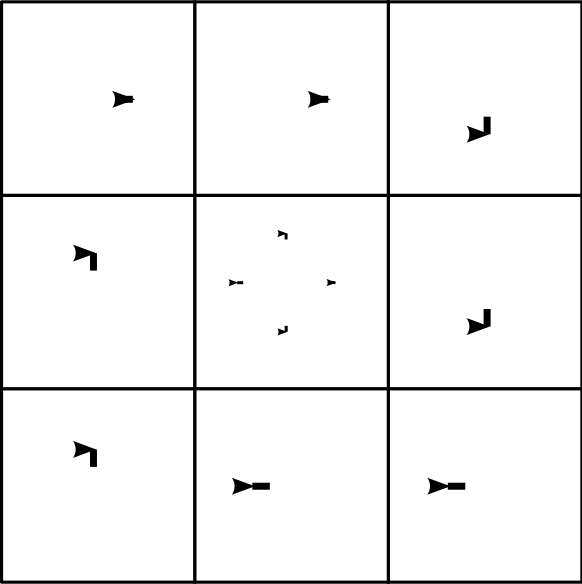
\includegraphics[width=0.8\columnwidth]{\visualspdf/frame/gridworld_around.pdf}
        \caption{W}
        \label{fig:gridwolrdgenericframesaround}
    \end{subfigure}
    \begin{subfigure}[b]{0.49\columnwidth}
        \centering
        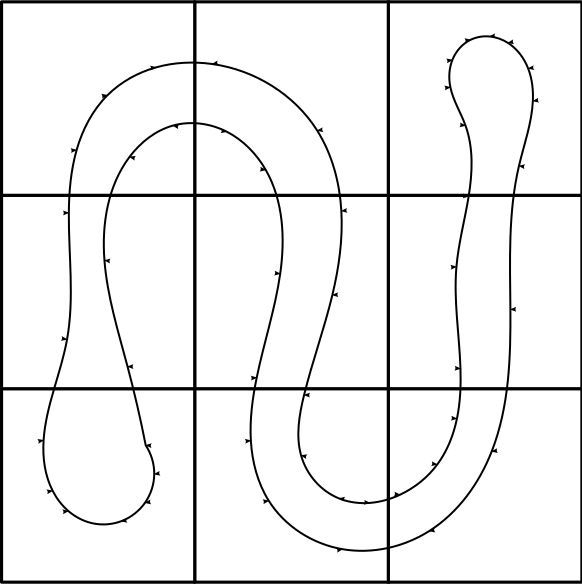
\includegraphics[width=0.8\columnwidth]{\visualspdf/frame/gridworld_loop.pdf}
        \caption{W}
        \label{fig:gridwolrdgenericframesloop}
    \end{subfigure}
\caption{Two examples of desired agent behavior that are harder to define in terms of rewards function.}
\label{fig:gridwolrdgenericframes}
\end{figure}

We note that it is always possible to represent the problems such that a fixed reward function allows to infer the policies of Figure~\ref{fig:gridwolrdgenericframesaround}~and~\ref{fig:gridwolrdgenericframesloop}. For Figure~\ref{fig:gridwolrdgenericframesaround} defining a reward function on the state-action space would be enough. For Figure~\ref{fig:gridwolrdgenericframesloop}, it is more challenging as the Markov properties are not respected, indeed it is necessary to known the previous position of the agent to predict its future position. Therefore the representation of the agent state should include the previous position of the agent, which increases the state space from 9 states to 81 states.

\subsection{No need for planning skills}

We provide an example of interaction frame where the agent do not need to know the optimal policy to interpret a signal with respect to a particular objective. In this frame, the goal of the robot is to locate one object or find one particular position in a 2D space. The teacher provide indication on the absolute direction of such object with respect to the agent position. As an example, we consider a teacher that indicates the cardinal direction of the object, i.e. the message to the robot is: \emph{``the object is North (South, West or East) with respect to your position''}.

We illustrate this frame in Figure~\ref{fig:cardinalframe}. The choice of the cardinal direction to send to the agent is modeled by a probabilistic models, where the probability of one cardinal direction is proportional to the angle between the target-agent direction and the cardinal direction considered.

\begin{figure}[!htbp]
    \centering
    
\includegraphics[width=0.8\columnwidth]{\visualspdf/frame/cardinal_frame.pdf}
    \caption{Example of the cardinal frame. The signal from the teacher indicates in which cardinal direction (N,S,W,E) the goal position or the object to reach is. There is a probabilistic model that describe the user behavior, such that the probability of generating a signal of meaning ``West'' is proportional to the angle between the agent position and the target position. This frame does not requires the agent to know how to reach the target position, but only its own position with respect to that goal.}
    \label{fig:cardinalframe}
\end{figure}

We defined as $\varphi_N$ the angle between the target-agent direction and the North cardinal direction, and respectively $\varphi_S$, $\varphi_W$, and $\varphi_E$ the angles with respect to the South, West, and East directions. The probability of that the user refers to the North cardinal direction is defined as follows:

\begin{equation}
    p(l^f = \emph{north}~|~\varphi_N) = 
    \begin{cases}
    (1 - \frac{2 \varphi_N}{\pi}) (1-\alpha) & if~\varphi_N < \frac{\pi}{2}\\
        \frac{\alpha}{K}  & \text{otherwise}\\
   \end{cases}
   \label{eq:cardinalframe}
\end{equation}
with $K$ the number of cardinal direction that do not satisfies the condition $\varphi_N < \frac{\pi}{2}$, which means K can take value of 2 or 3 only. $\alpha$ is the error rate of the user. Finally, we consider unsigned angles only within the $[0, \pi]$ intervals only, meaning that angles of $\frac{-\pi}{2}$ or $\frac{3\pi}{2}$ are taken as $\frac{\pi}{2}$. The same equation applies for all cardinal direction and should maintain the following properties $\sum_{c \in \{N,S,E,W\}} p(l^f = c |\varphi_c) = 1$.

In practice, if we consider our visual representation of Figure~\ref{fig:cardinalframe}, we obtain the following angle measurements: $\varphi_N = \frac{9\pi}{22}$, $\varphi_S = \frac{13\pi}{22}$, $\varphi_W = \frac{20\pi}{22}$, and $\varphi_E = \frac{\pi}{11}$. In that case $K = 2$. If we consider $\alpha = 0$, we obtain the following probabilities values: $p(l^f = \emph{north}~|~\varphi_N) = 0.18$, $p(l^f = \emph{south}~|~\varphi_S) = 0$, $p(l^f = \emph{west}~|~\varphi_W) = 0$, and $p(l^f = \emph{east}~|~\varphi_E) = 0.82$, which we represent as a vector $[0.18,0,0,0.82]$. If we account of some probability of errors from the teacher, taking for example $\alpha = 0.05$, we obtain the following vector of probability: $[0.17, 0.025, 0.025,0.78]$.

We will use this frame in our experiment of section~\ref{chapter:limitations:continuoushypothesis}. Note that the same frame can apply with different referential, instead of the cardinal direction, one could refer to the direction with respect the robot orientation, or with respect to the position of the human teacher in the room, etc.

\subsection{Asynchronous instructions}

The interaction between our users and our robot would be easier if the robot could act continuously and the human would provide instruction when he deemed necessary. For example, in our pick and place scenario of chapter~\ref{chapter:lfui} it is boring for the user to provide feedback after each movement of the robot, it would be easier to wait the robot has displaced a cube to an other location. In addition, in some domains, the frequency of action is to high to afford waiting for a feedback signal between each action. Either the action would be so small that the user would not be able to judge the action, either the interaction flow would be dramatically affected by the many pauses in the task execution.

To allow for continuous operation of the robot, asynchronous delivery of signals should be accepted. A potential avenue is to consider a temporal function that distribute a signal event across some subset of previous robot events. This method has been used by Bradley Knox et al. in their TAMER framework \cite{knox2009interactively} using a data from a study of the distribution of human response times \cite{hockley1984analysis}.

\subsection{Including social clues}

As for tackling the problem of asynchronous instructions, information known to be true for most interaction scenario can be included in the frame definition.  Such as whether the human is looking at the scene or not, but also the presence of other persons in the room, or that some objects are hiding parts of the world to the human eye, etc.

%!TEX root = ../../thesis.tex
\section{Continuous state space}
\label{chapter:limitations:continousstate}

\question{How to deal with continuous states?}

As for now, our algorithm assumes the world can be represented by a limited number of discrete states. In this section we extend our algorithm to a continuous world, but still consider discrete actions. In addition, we present a new interaction frame that combines the feedback and guidance frames. We investigate how our algorithm scales to such problem and how different exploration strategies perform.

\subsection{Experimental System}

We consider a puddle world, in which an agent must reach a goal region while avoiding a penalty region. We consider a 2 dimensional puddle world with each dimension ranging between 0 and 1. The state of the agent can be any coordinate in the 2D world. Agent' actions are discrete and represent steps in either North, South, East, West direction. One step length is sampled from a normal distribution of mean 0.1 and standard deviation 0.01.

As in the experiment of chapter~\ref{chapter:lfui}, we consider speech as the modality for interacting with the robot and we reuse the dataset presented in section~\ref{chapter:lfui:speechdata}. The interaction between the agent and the teacher follows a turn taking social behavior, where the agent is performing an action and waits for a feedback or guidance signal to continue. We only consider a Gaussian classifier.

\paragraph{Task Representation} 

To define the set of possible tasks we project a 5x5 regular grid on top of the continuous world. One task is represented by a +1 reward in one of the 25 projected squares and a -100 reward in three consecutive (vertically or horizontally) squares. +1 and -100 area can not overlap (see figure~\ref{fig:puddle} for an example). The set of possible tasks is defined as all possible combinations of such reward function, for a total of 660 hypotheses.

Our algorithm only needs to have access to the optimal policies to be able to interpret a signal with respect to the feedback or guidance frame. We use the MDP framework to compute the corresponding policies. The world being continuous we use the tile coding function approximation \cite{sutton1998reinforcement}, with 10 overlapping 50x50 regular grids. A Q-Learning algorithm \cite{watkins1992q} is used to compute the Q-Values, with a discount rate of 0.99 and a learning rate of 0.01. The optimal policies are then defined as greedy according to the Q-Values.

\paragraph{Mixed feedback and guidance frame}

In previous chapters, we considered only the feedback or the guidance frame separately. Such limitation can be restrictive for the user, we  now consider the case where the teacher can use both feedback and guidance signal. We define as $F$ as the set of meanings associated to the feedback meanings (i.e. ``correct'' and ``incorrect''), and $G$ the set of meanings associated to the guidances meanings (i.e. ``action 1'', ``action 2'', ...). Extending our algorithm to cases where possible meanings include both feedback and guidance (i.e. $l^f \in \{F \cup G\}$) requires a probabilistic model of how the teacher distributes feedback and guidance signals. This model must hold the following property $\sum_{l \in \{F \cup G\}} p(l^f = l|s,a,\xi)~=~1$. We define a variable $\phi$ that represents the probability of the user providing a feedback signal at each step, i.e. $p(l^f \in F) = \phi$, which implies $p(l^f \in G) = 1 - \phi$.

Under this new definition we can change our frame definition to:

\begin{eqnarray}
    p(l^f = l|s,a,\xi) = 
        \begin{cases} 
            \phi~p(l^f = l|s,a,\xi) &\mbox{for } l \in F \\
            (1- \phi)~p(l^f = l|s,\xi) & \mbox{for } l \in G
        \end{cases}
        \label{eq:mixedfeedbackguidance}
\end{eqnarray}
where Equation~\ref{eq:feedbackframe} holds for the feedback component (for $l \in F$) and Equation~\ref{eq:guidanceframe} holds for the guidance component (for $l \in G$). 

We assume the mixing parameter $\phi$ is known in advance. We set $\phi$ to 0.5 meaning the user is providing feedback half of the time and guidance the other half of the time. 

\paragraph{Exploration strategies}

We investigate four different agent behaviors: \begin{inparaenum}[a)] \item random, \item $\epsilon$-greedy, \item myopic uncertainty based exploration, which aims at selecting the action that is the most uncertain in the current state, and \item full uncertainty based exploration which requires an uncertainty map to decide what to explore next. \end{inparaenum} 

As we are in a continuous domain, we can not compute the full uncertainty for each state as presented in chapter~\ref{chapter:planning}, we therefore approximate this process. Extensions of the general problem already exist for the continuous state problem \cite{nouri2010dimension,Hester13aamas} and we will rely on a sampling based method. One hundred random states are generated and evaluated in terms of their uncertainty. Each sampled state is associated to a reward value proportional to its uncertainty which is propagated to neighborhood states by using a fixed Gaussian kernel. We use as amplitude the uncertainty value and a diagonal covariance matrix of value 0.01 for each component. The resulting approximated uncertainty map is then used as a reward function. By solving the corresponding MDP, using for instance Q-Learning, the agent plans its actions to visit the most uncertain regions. We decided to use an $\epsilon$-greedy policy on the Q-values. In the following experiment, the agent will use an exploration ratio $\epsilon$ equal to $0.1$.

\subsection{Results}

We present results from 75 runs of our experiment, where for each run we randomly choose a task to teach from the set of hypotheses, as well as the initial state of the agent. The simulated teacher makes 10 percent of teaching mistakes, i.e. sending an erroneous signal 10 percent of the time. For each experiment, we compute the likelihoods every 15 steps and performs a total of 35 updates, for a total of 525 iterations. Figure~\ref{fig:continuousstateRmax} shows the average evolution of the taught task hypothesis likelihood.

\begin{figure}[!htbp]
  \centering
  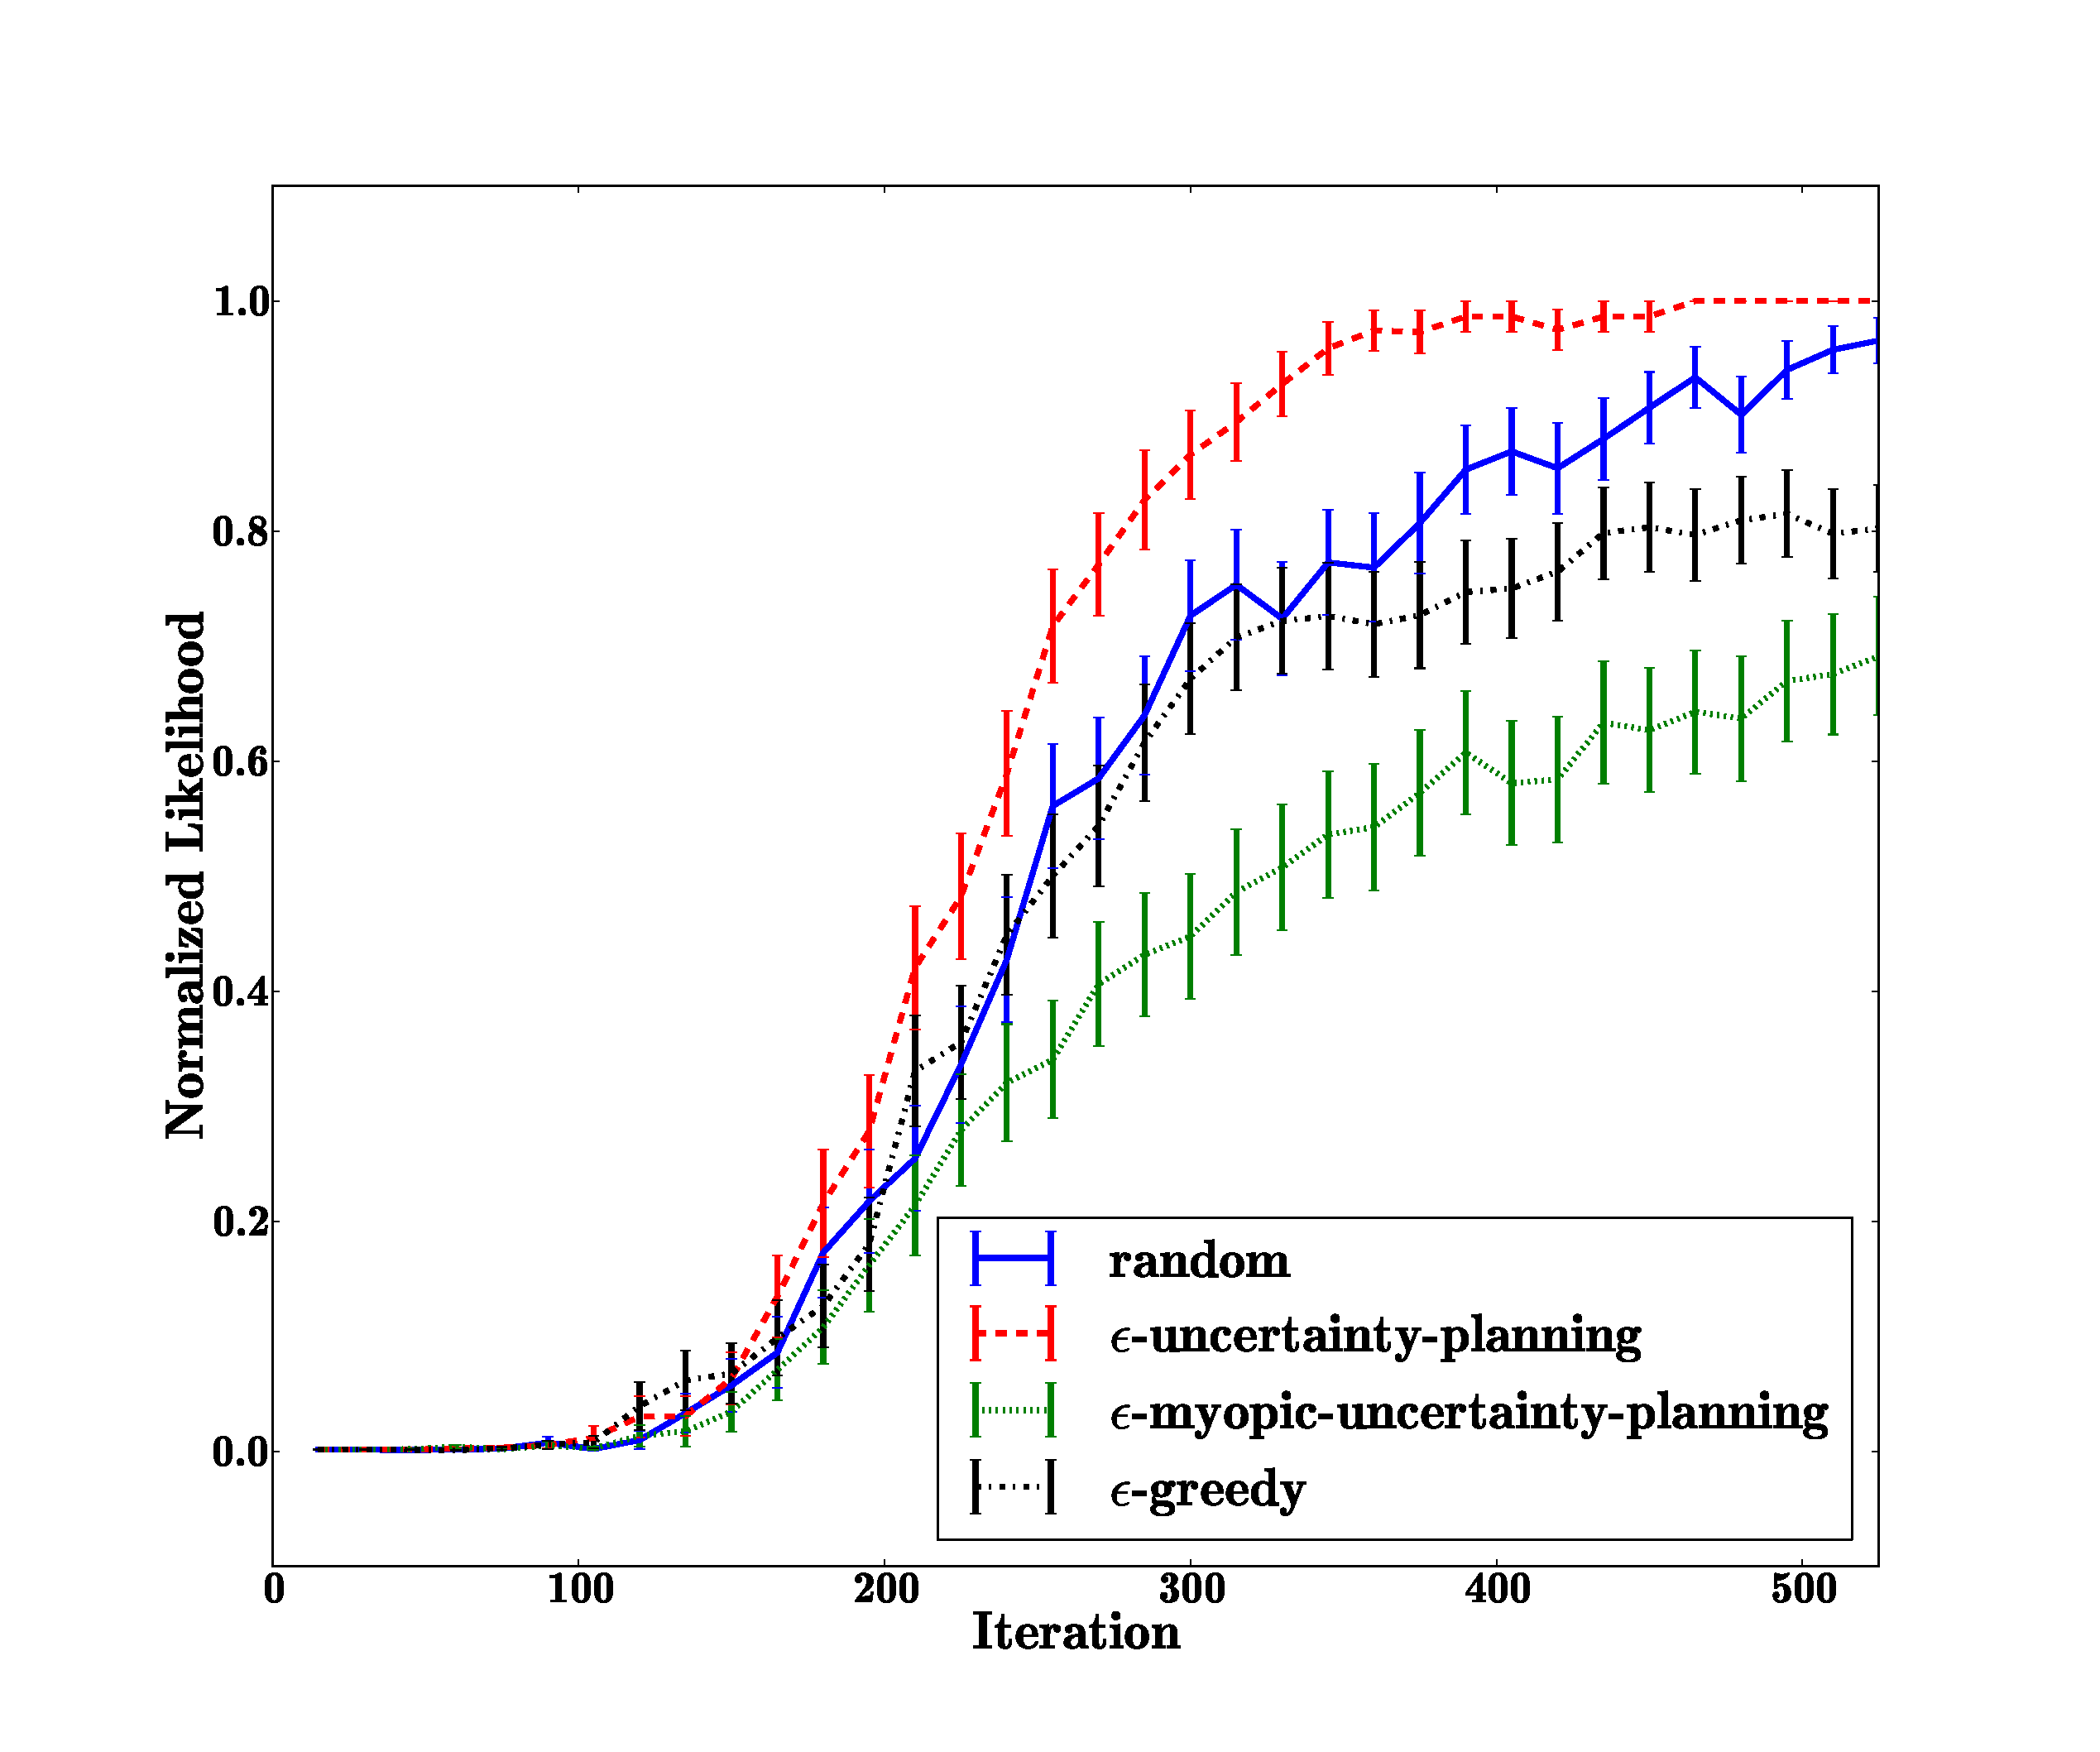
\includegraphics[width=\plotsize\columnwidth]{\imgpath/continuous_state/continuous}
  \caption{Taught hypothesis normalized likelihood evolution (mean + standard error) thought iteration using a Gaussian classifier. Comparison of different exploration strategies. Uncertainty based exploration method, which plan on the long term, performs significantly better on average.}
  \label{fig:continuousstateRmax}
\end{figure}

These results show that our algorithm can learn a task in a continuous world from unlabeled and noisy instructions whose possible meanings are both feedback and guidance and 10 percent of the instructions were teaching mistakes. The uncertainty based planning strategy outperforms random action selection. Interestingly, myopic uncertainty based strategy, which is also based on our uncertainty measure, is not efficient. This result illustrates that, when considering the agent as not being able to teleport, a long term planning approach is more suited to explore efficiently the state space than a short term vision by selecting the next action with higher immediate reward, i.e. higher uncertainty. 

% Finally $\epsilon$-greedy performs less efficiently than in the first setup. This is due to the properties of our new set of hypothesis where many hypothesis shared an identical positive reward area but have different puddle zone.

Figure~\ref{fig:continuousstateUncertaintyMap} shows the evolution of the estimated uncertainty map for one run of the experiment. For each uncertainty map, the agent plans its actions to reach a maximal uncertainty region. The maximum uncertainty value decreases as the agent is correctly estimating the task.

\begin{figure}[!p]
  \centering
      \begin{subfigure}[b]{0.35\columnwidth}
          \centering
          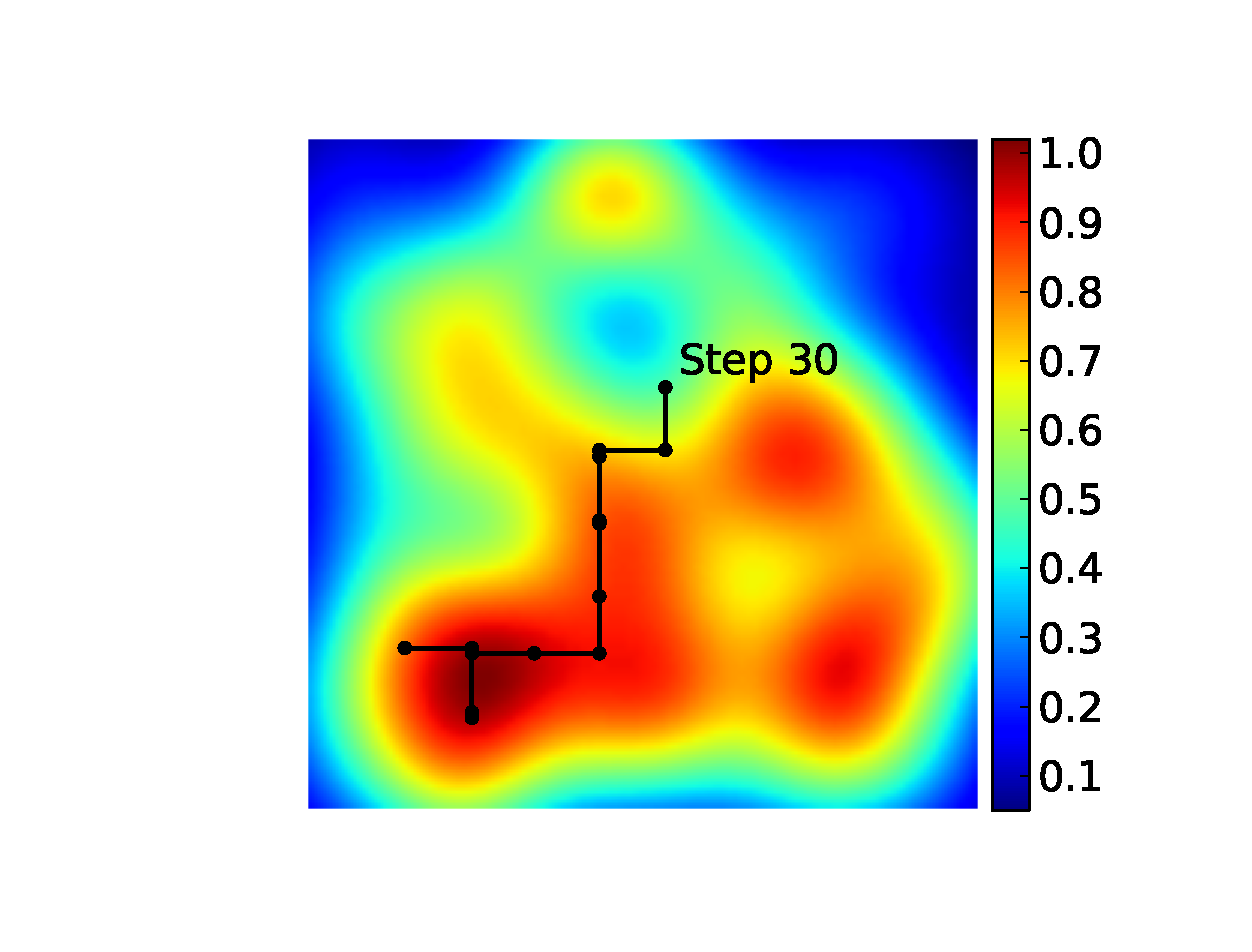
\includegraphics[trim=5cm 1.5cm 1.5cm 1.5cm, clip=true, width=\columnwidth]{\imgpath/continuous_state/30}
          \caption{After 30 iterations.}
          \label{fig:30}
      \end{subfigure}
      \begin{subfigure}[b]{0.35\columnwidth}
          \centering
          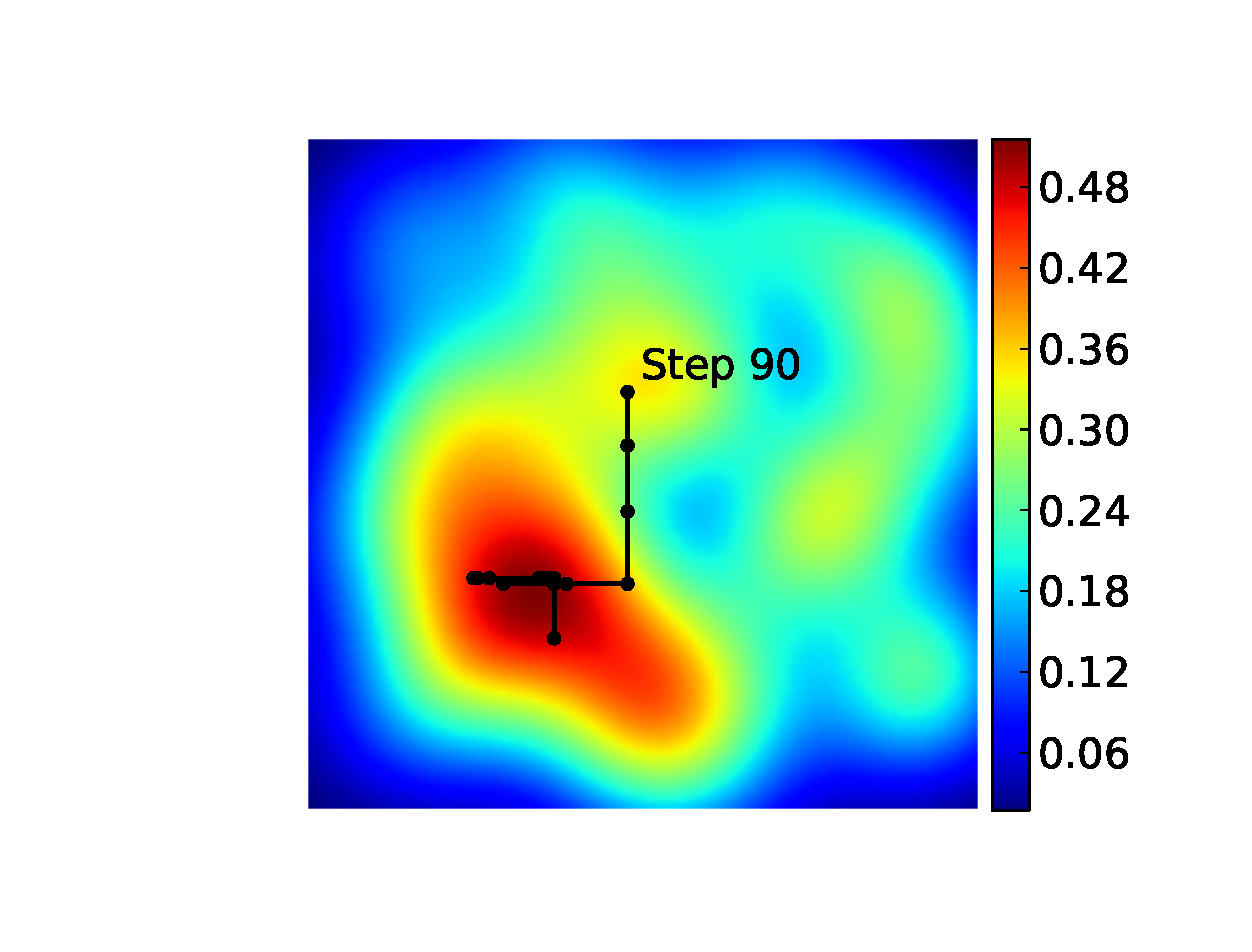
\includegraphics[trim=5cm 1.5cm 1.5cm 1.5cm, clip=true, width=\columnwidth]{\imgpath/continuous_state/90}
          \caption{After 90 iterations.}
          \label{fig:90}
      \end{subfigure}\\
      \begin{subfigure}[b]{0.35\columnwidth}
          \centering
          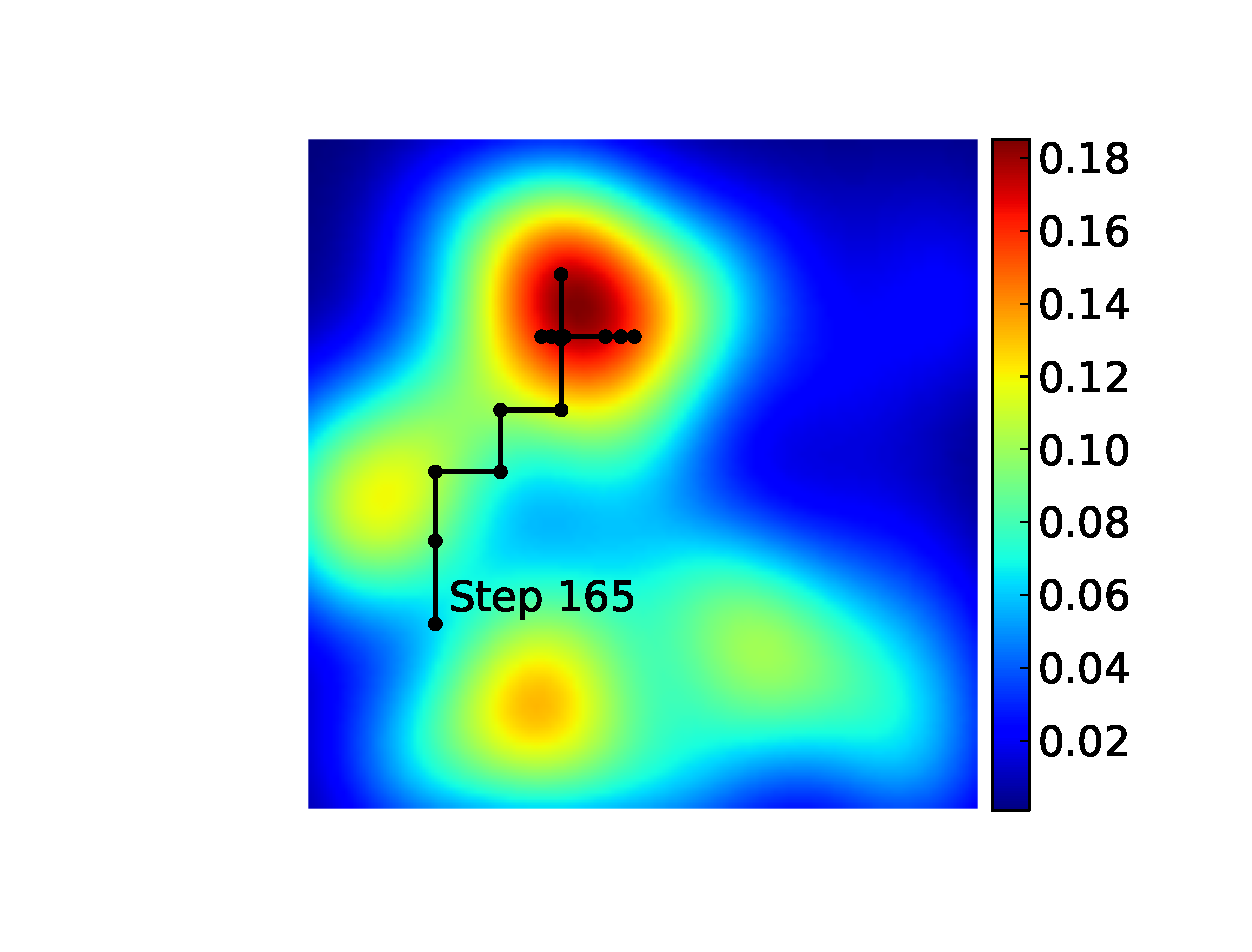
\includegraphics[trim=5cm 1.5cm 1.5cm 1.5cm, clip=true, width=\columnwidth]{\imgpath/continuous_state/160}
          \caption{After 165 iterations.}
          \label{fig:165}
      \end{subfigure}
      \begin{subfigure}[b]{0.35\columnwidth}
          \centering
          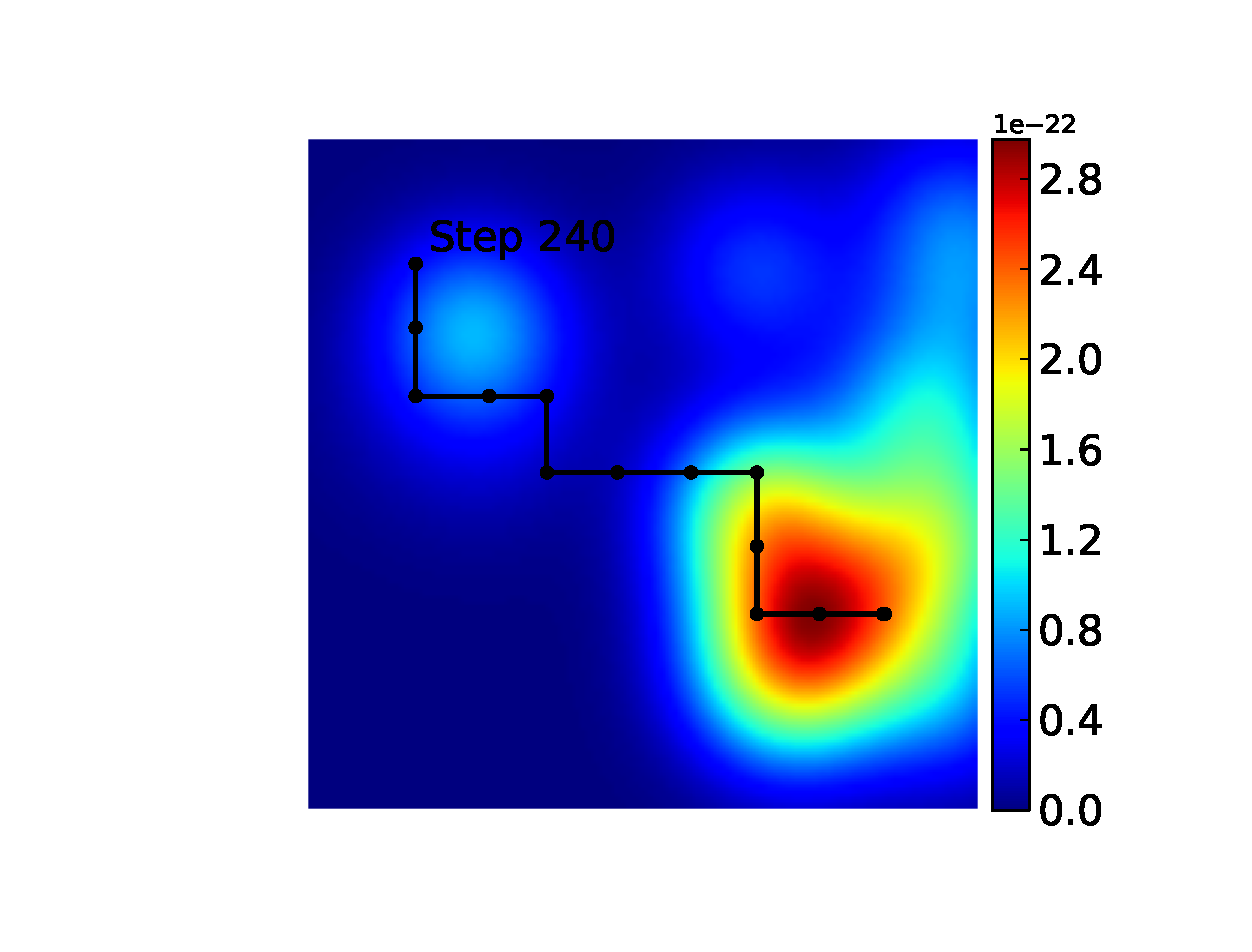
\includegraphics[trim=5cm 1.5cm 1.5cm 1.5cm, clip=true, width=\columnwidth]{\imgpath/continuous_state/240}
          \caption{After 240 iterations.}
          \label{fig:240}
      \end{subfigure}\\
      \begin{subfigure}[b]{0.25\columnwidth}
          \centering
          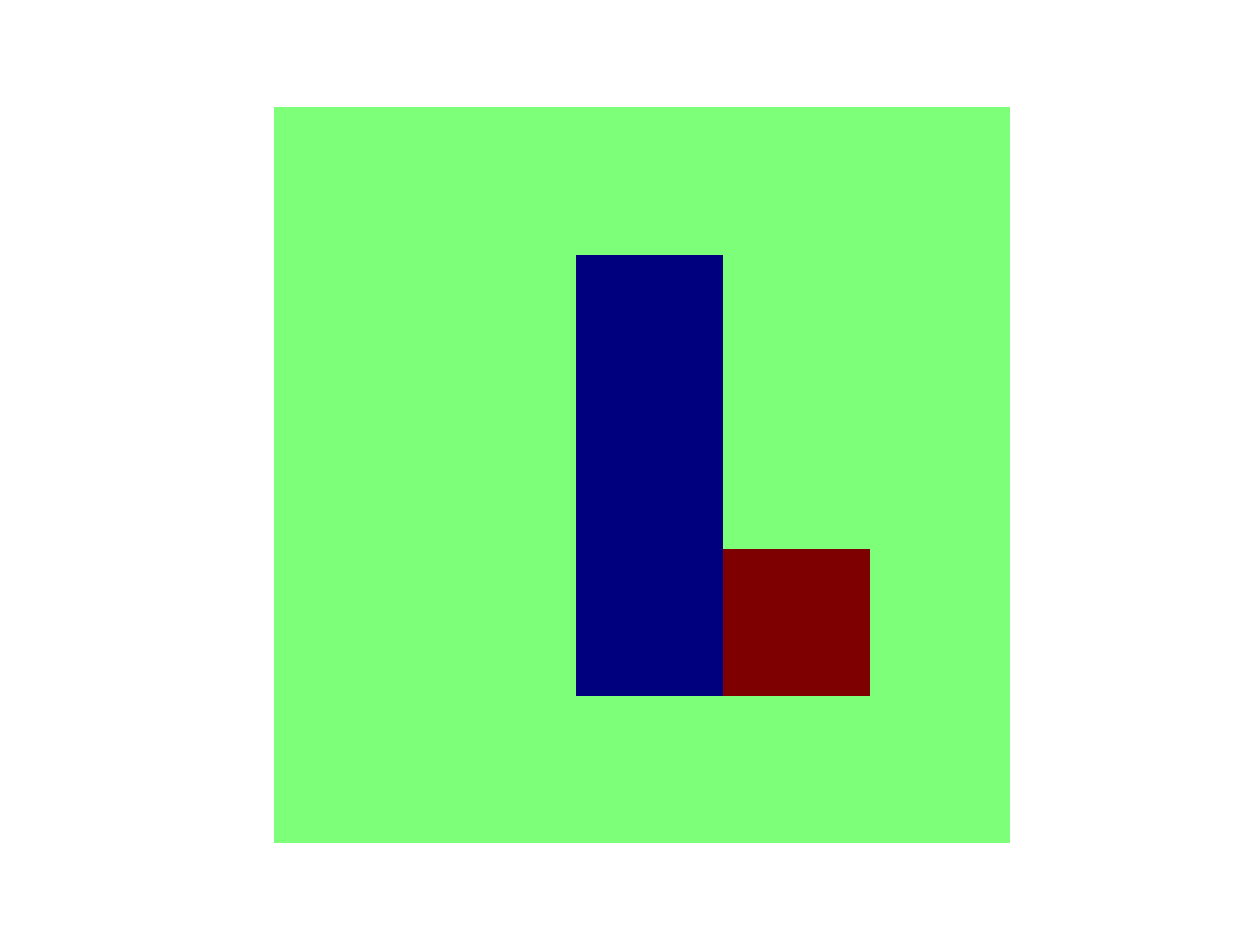
\includegraphics[trim=4cm 1cm 3.5cm 1cm, clip=true, width=\columnwidth]{\imgpath/continuous_state/puddle}     
          \caption{Puddle world used by the teacher.}
          \label{fig:puddle}
      \end{subfigure}
      \begin{subfigure}[t]{0.45\columnwidth}
          \centering
          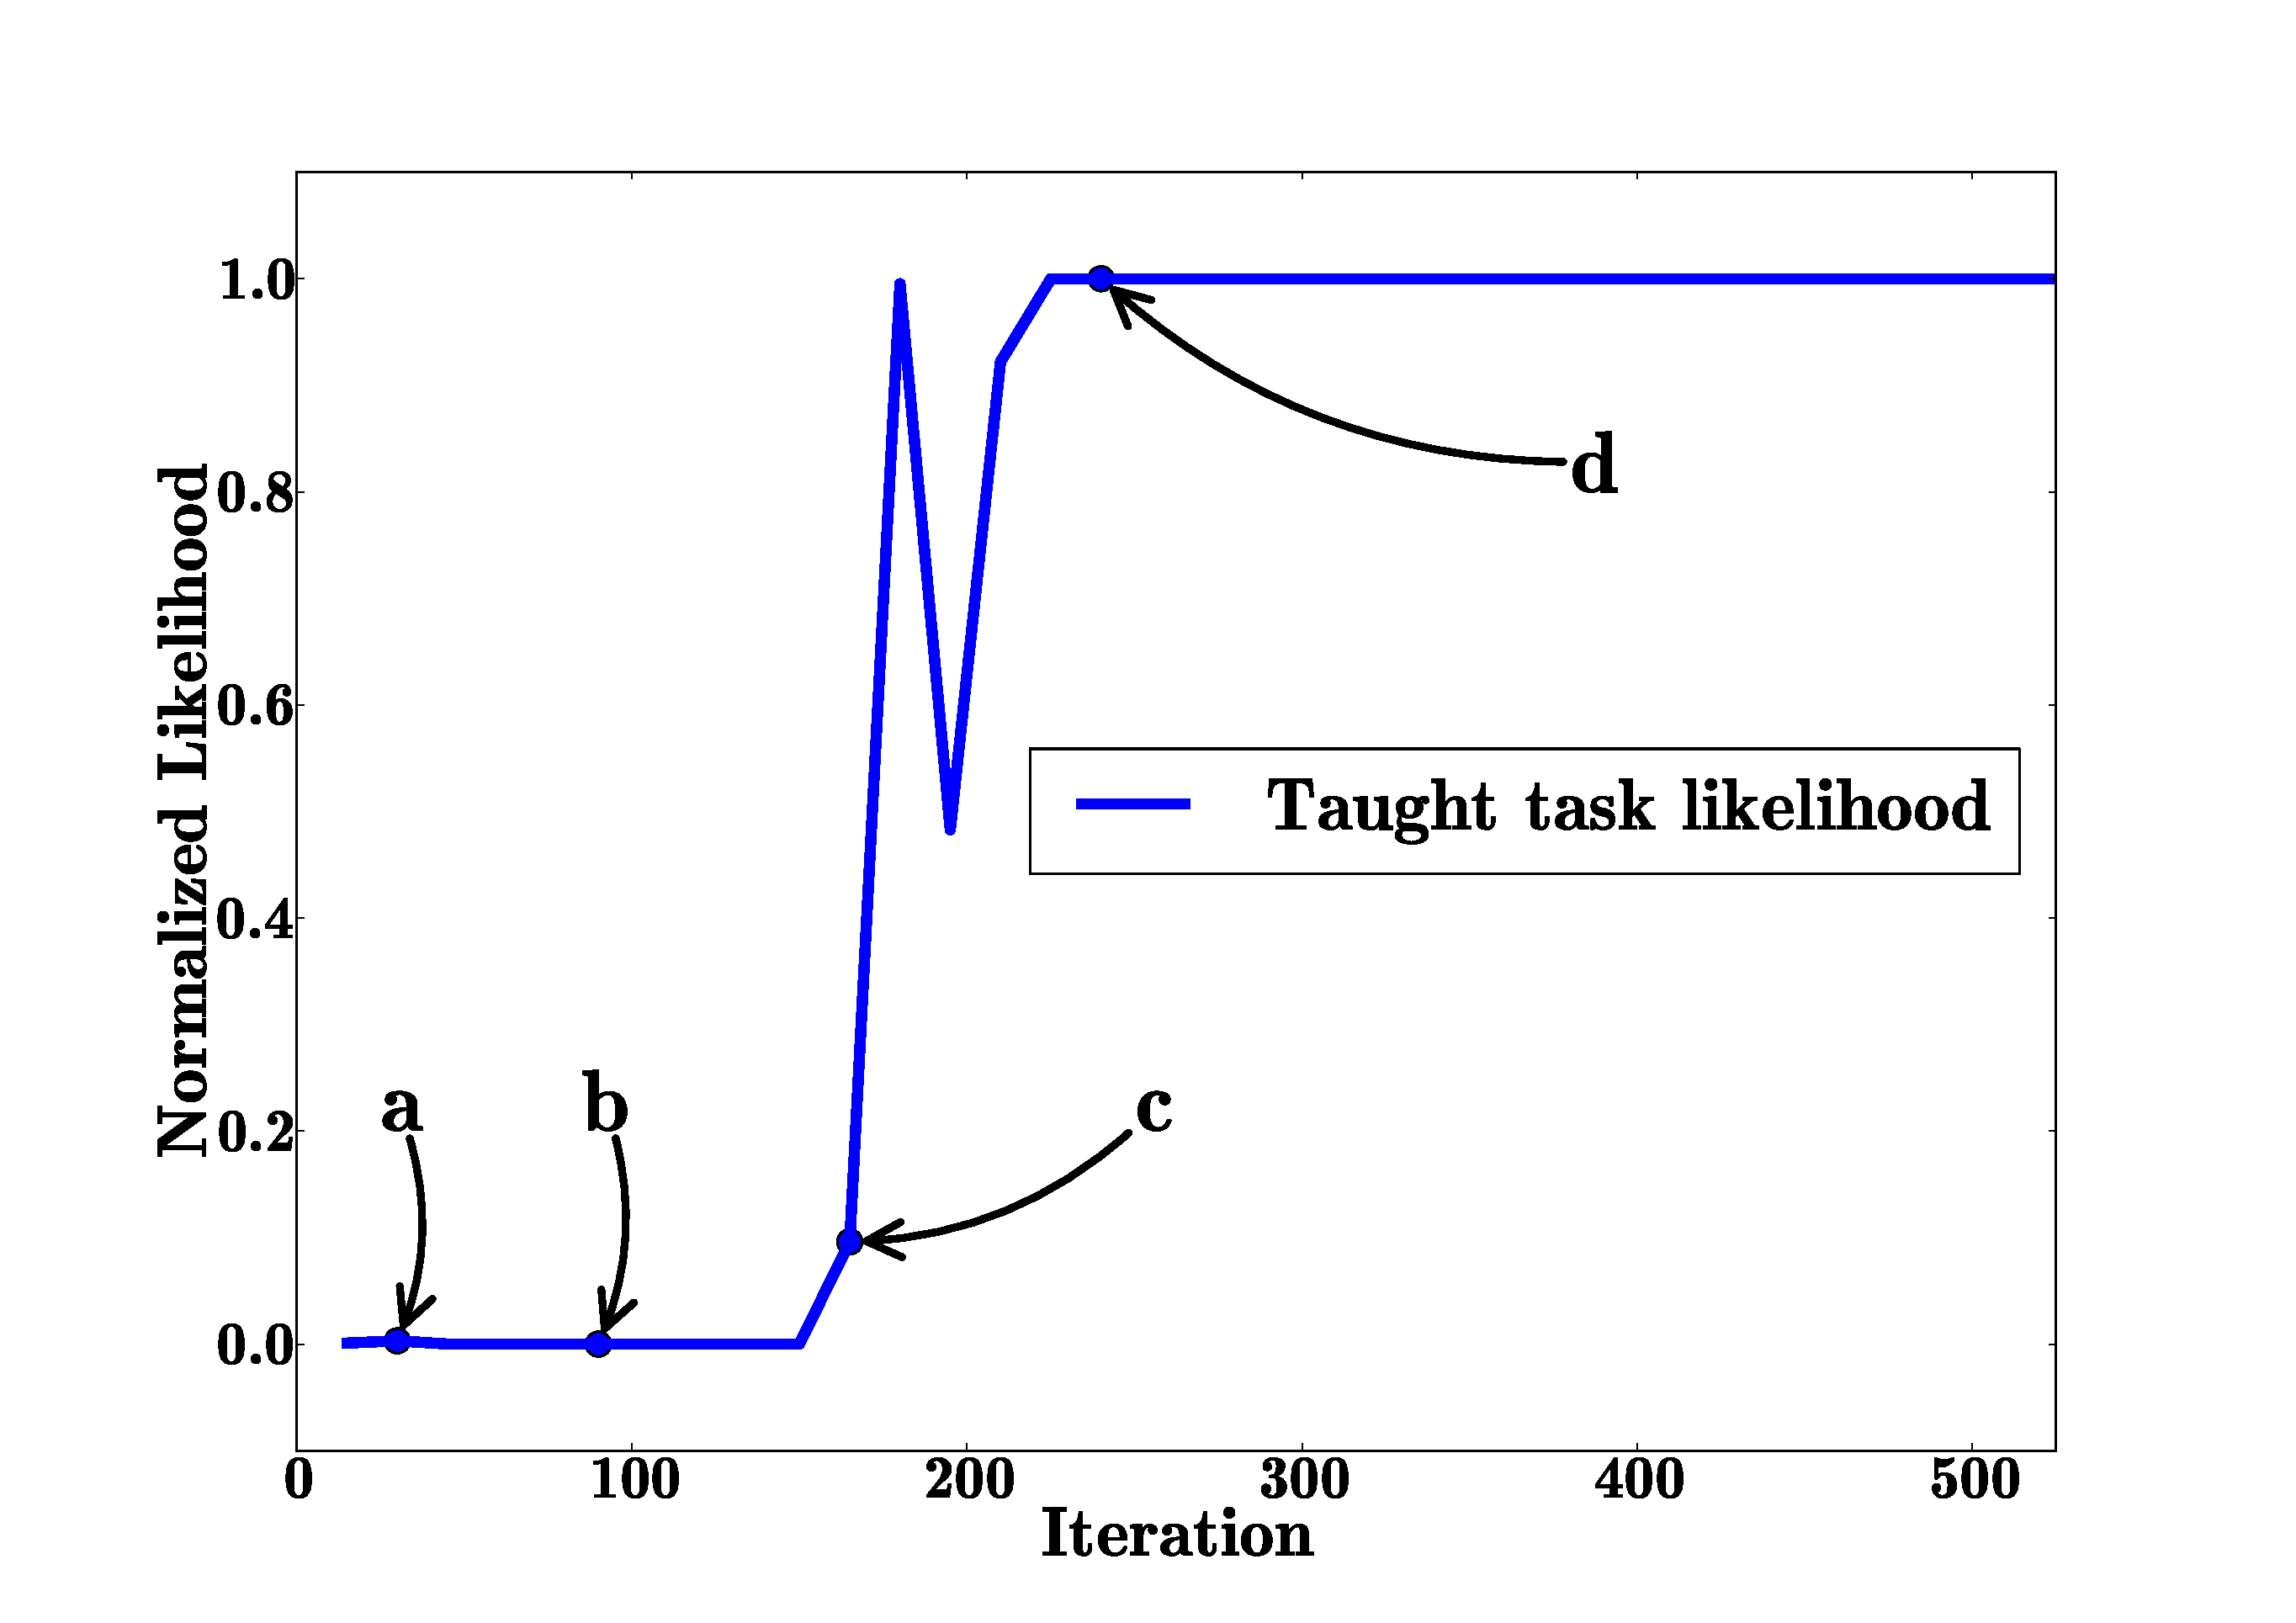
\includegraphics[trim=2cm 1cm 3cm 2cm, clip=true, width=\columnwidth]{\imgpath/continuous_state/evo}
          \caption{Taught hypothesis normalized likelihood evolution.}
          \label{fig:evo}
      \end{subfigure}
        
  \caption{Log Uncertainty maps after a) 30, b) 90, c) 165 and d) 240 iterations. e) shows the puddle world chosen by the teacher and f) shows the learning progress and the frame associated to each of the uncertainty map. In order to display the differences between log values, we bounded the color map between -5 and 0, which correspond to uncertainty values between 0.0067 and 1. Some log values, especially for d), are lower than -5 and are displayed in the same color as -5. Best shown in color.}
  \label{fig:continuousstateUncertaintyMap}
\end{figure}

\newpage 

\subsection{Discussion}

We have shown how our algorithm could be applied to continuous state domains and seen that, given the interaction frame considered, our algorithm only needs to have access to the optimal policies associated to each task to be able to interpret a signal. Therefore any method that allow to compute a policy for continuous domains could be used. The only problem is then related to the computational cost of those methods than to the formalism of this work. We will see in next section that, for some specific frames and worlds, it is not always needed for the robot to know the optimal policies to interpret the teaching signals from the human, which can considerably reduce the computational cost of running our algorithm.
%!TEX root = ../../thesis.tex

\section{Continuous set of hypothesis}
\label{chapter:limitations:continuoushypothesis}

\question{How to relax the assumtion that \\ the correct task belong to a known finite set of hypothesis?}

In order to make the learning problem tractable, we assumed that the robot learner knows that the task to be learnt can be approximated by one task among a pre-defined set of tasks. Indeed, without constraining the space of possible tasks, an infinite number of tasks may explain the particular teaching data received. In practice, the number of pre-defined tasks in the experiment was still relatively large, allowing a certain level of flexibility. Yet, it would be highly desirable to extend the possibility to deal with continuous task representation, allowing potentially infinite task spaces. 

A potential avenue to address this is to constrain search through a combination of regularization and particle filter approaches. In the following of this section, we present a simple particle filter based algorithm that allow an agent to identify a task from unlabeled instruction and considering an infinite set of hypothesis. The agent lives in a 2 dimensional continuous state space and should identify which  coordinate it should reach, among the infinite number of possible coordinates.

\subsection{World and task}

We consider an agent living in a 2 dimensional continuous space bounded between 0 and 1 in both dimensions. A teacher is providing indication about the orientation of the goal state compared to the robot state by drawing some patterns on a tablet. Those directions can only be selected among of the four cardinal directions that are the directions of north, east, south, and west. The teacher wants the robot to reach a particular state, that can be any position in the continuous 2 dimensional space. The robot is able to teleport itself to any location of the space to receive a new indication.

We still consider a strong a priori knowledge on the space of task, which is that there is only one goal state. This is a very strong a priori regularization on the complexity of the problem. Considering there could be several goal positions, depending for example on the current position of the agent, would increase dramatically the search space; it would then be likely that many hypothesis of different complexity would explain well the observed data. In such case a rule for regularizing the hypothesize task solutions would be needed.

\subsection{Interaction frame}

We define the cardinal direction frame define 
In this frame, the user provide an information about the cardinal direction of the goal state with respect the current agent position. The agent does not need to know the optimal policy to interpret a signal but only its current state. The teacher provide indication on the absolute direction of the goal state with respect to the agent position. As an example, we consider a teacher that indicates the cardinal direction of the object, i.e. the message to the robot is: \emph{``the object is North (South, West or East) with respect to your position''}.

We illustrate this frame in Figure~\ref{fig:cardinalframe}. The choice of the cardinal direction to send to the agent is modeled by a probabilistic model, where the probability of one cardinal direction is proportional to the angle between the target-agent direction and the cardinal direction considered.

\begin{figure}[!htbp]
    \centering
    
\includegraphics[width=0.8\columnwidth]{\visualspdf/frame/cardinal_frame.pdf}
    \caption{Example of the cardinal frame. The signal from the teacher indicates in which cardinal direction (N,S,W,E) is the target position. There is a probabilistic model that describe the user behavior, such that the probability of generating a signal of meaning ``West'' is proportional to the angle between the agent position and the target position. This frame does not requires the agent to know how to reach the target position, but only its own position with respect to that goal.}
    \label{fig:cardinalframe}
\end{figure}

We defined as $\varphi_N$ the angle between the target-agent direction and the North cardinal direction, and respectively $\varphi_S$, $\varphi_W$, and $\varphi_E$ the angles with respect to the South, West, and East directions. The probability that the user refers to the North cardinal direction is defined as follows:

\begin{equation}
    p(l^f = \emph{north}~|~\varphi_N) = 
    \begin{cases}
    (1 - \frac{2 \varphi_N}{\pi}) (1-\alpha) & if~\varphi_N < \frac{\pi}{2}\\
        \frac{\alpha}{K}  & \text{otherwise}\\
   \end{cases}
   \label{eq:cardinalframe}
\end{equation}
with $K$ the number of cardinal direction that do not satisfies the condition $\varphi_N < \frac{\pi}{2}$, which means K can take value of 2 or 3 only. $\alpha$ is the error rate of the user. Finally, we consider unsigned angles only within the $[0, \pi]$ intervals, meaning that angles of $\frac{-\pi}{2}$ or $\frac{3\pi}{2}$ are taken as $\frac{\pi}{2}$. The same equation applies for all cardinal direction and should maintain the following properties $\sum_{c \in \{N,S,E,W\}} p(l^f = c |\varphi_c) = 1$.

In practice, if we consider our visual representation of Figure~\ref{fig:cardinalframe}, we obtain the following angle measurements: $\varphi_N = \frac{9\pi}{22}$, $\varphi_S = \frac{13\pi}{22}$, $\varphi_W = \frac{20\pi}{22}$, and $\varphi_E = \frac{\pi}{11}$. In that case $K = 2$. If we consider $\alpha = 0$, we obtain the following probabilities values: $p(l^f = \emph{north}~|~\varphi_N) = 0.18$, $p(l^f = \emph{south}~|~\varphi_S) = 0$, $p(l^f = \emph{west}~|~\varphi_W) = 0$, and $p(l^f = \emph{east}~|~\varphi_E) = 0.82$, which we represent as a vector $[0.18,0,0,0.82]$. If we account of some probability of errors from the teacher, taking for example $\alpha = 0.05$, we obtain the following vector of probability: $[0.17, 0.025, 0.025,0.78]$.

We will use this frame in our experiment with $\alpha = 0.01$. Note that the same frame can be used with different referential, instead of the cardinal direction, one could refer to the direction with respect the robot orientation, or with respect to the position of the human teacher in the room.

\subsection{Finger movements datasets}

We will present results using two different datasets made of finger movements performed on a tablet. 

Our first dataset shown in Figure~\ref{fig:fingerdatasetdirection} is build from a user generating directional trajectories starting from the center of the tablet and going toward the edges of the tablet. We considered four different movements, one toward each edge, representing the four cardinal directions that are the directions of north, east, south, and west.

\begin{figure}[!htbp]
\centering
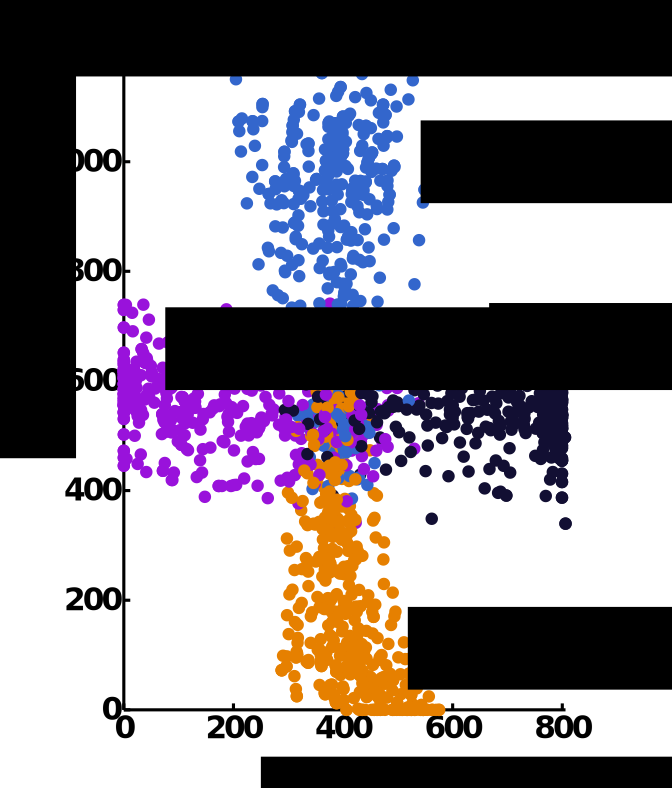
\includegraphics[width=\signalwidth\columnwidth]{\visualspdf/worlds_and_datasets/finger_signals_color.pdf}
\caption{N}
\label{fig:fingerdatasetdirection}
\end{figure} 

\newpage

Our second dataset shown in Figure~\ref{fig:fingerdatasetsigns} is build from a user drawing the cardinal letters (N, S, W, and E) in the middle of the tablet.

\begin{figure}[!htbp]
\centering
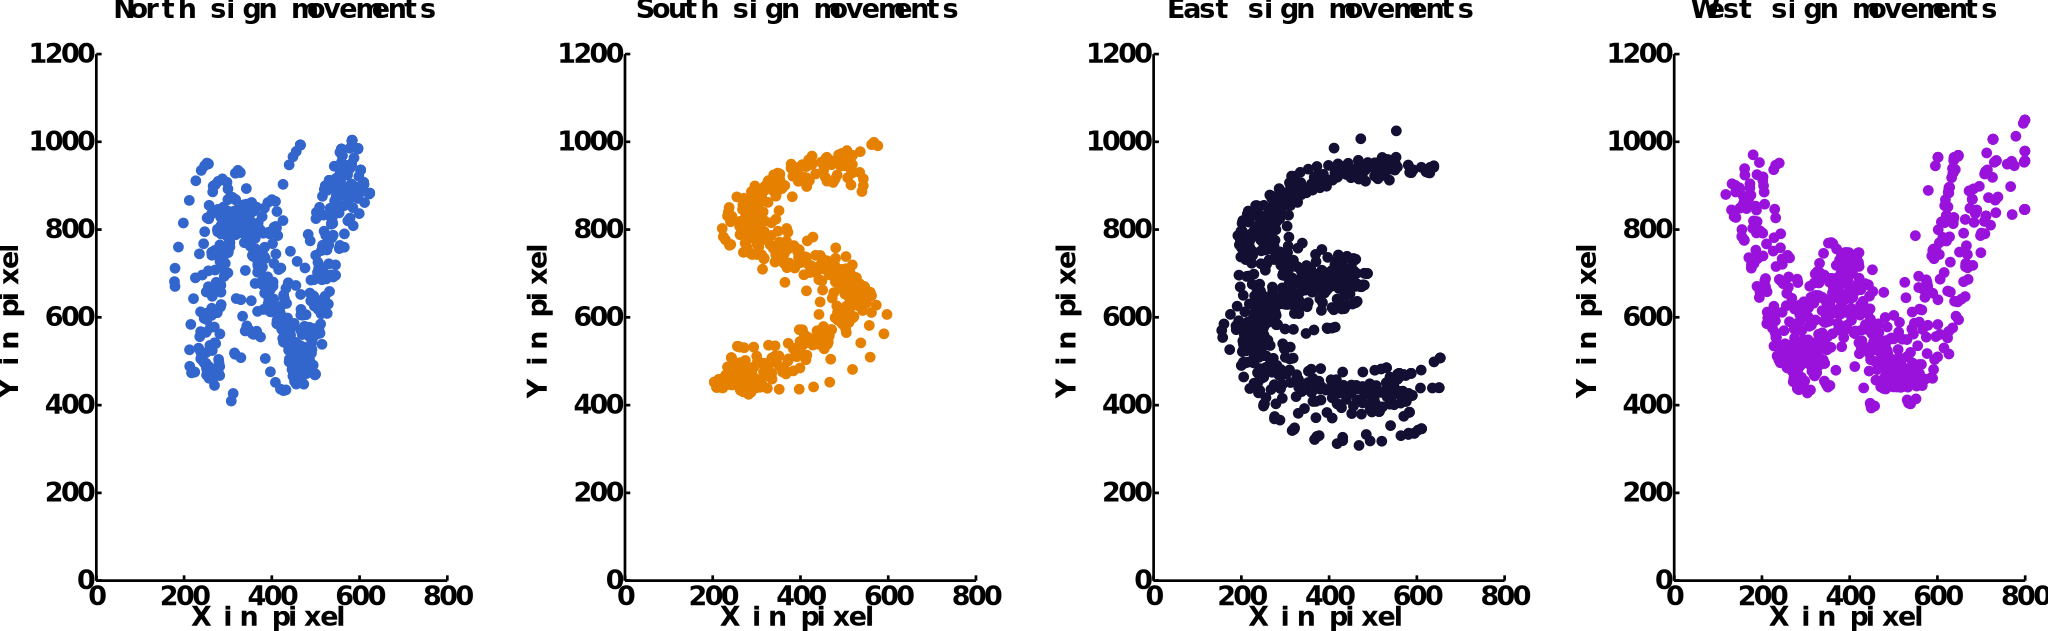
\includegraphics[width=\columnwidth]{\visualspdf/worlds_and_datasets/finger_signals_color_signs.pdf}
\caption{N}
\label{fig:fingerdatasetsigns}
\end{figure} 

To represent those trajectories, our feature vector is composed of 11 dimensions, encoding:
\begin{itemize}
   \item The start X and Y positions (2 features)
   \item The end X and Y positions (2 features)
   \item The delta position between start and end position for X and Y coordinate (2 features)
   \item The median X and Y positions (2 features)
   \item The distance between start and end position (1 feature)
   \item The total distance traveled by the finger (1 feature)
   \item The average speed of the finger (1 feature)
\end{itemize}

Using this representation we achieve 100 percent accuracy on the directional movements dataset and 99 percent accuracy on the cardinal signs dataset, using a simple Gaussian classifier with one Gaussian per class.

We remind that each movement has no a priori meaning for the robot. For example, in our simulation we may use the ``W'' sign signals to mean the goal state is north to the agent position.

\subsection{Evaluating task likelihood}

As there is an infinity of possible goal states, the agent can not estimate the probability of all possible tasks in parallel. We will rely on a particle filter based approach \cite{gordon1993novel,doucet2009tutorial,thrun2002particle}. The main idea consist of sampling a finite number of tasks and computing a confidence measure for each of those tasks. Given the ranking between them, we will apply a resample step which consists of keeping some of the best tasks and sample new ones. More details are provided in next subsection~\ref{chapter:limitations:continoushypothesis:particlefilter}, we present in this subsection how we estimate the probability of each sampled task.

Our algorithm, as presented so far, was cumulatively accumulating evidence for each task and was updating the likelihood of each task on a step by step basis. However, for this experiment, as the task hypotheses are changing every step, we can not update the likelihood of each task on a step by step basis, as described in Equation~\ref{eq:matchingfiltercrossvalidation}. This approach allowed us to reduce the computational cost of our algorithm so as to be able to run our experiments in a reasonable amount of time. A possible option would be to use Equation~\ref{eq:matchingcrossvalidation}, but it would requires to train a 100000 classifiers at iteration 200, which was not feasible in reasonable time.

We selected an other method which rely on sampling different classifiers from a meta-classifier. It allows to generate classifiers at a low computational cost. Then, given many classifiers for each task, we can compare the likelihoods predicted by these classifiers and rank the task by a statistical test. We describe each step of this process in the following paragraphs.

The first step is to compute a ``meta'' model which encodes a distribution of probability on the classifier parameters, i.e. which encodes a probability distribution over the mean and covariance of each class. To do so, and given that we are using multivariate normal distributions, we use a noninformative (Jeffrey's) prior \cite{gelman2003bayesian} to estimate the probability distribution over the means and covariances:

\begin{eqnarray}
p(\mu_l|D) & = & t_{n-d}(\mu| \bar{x}_l, \frac{S_l}{n(n-d)})
\label{eq:jeffreysmean}
\end{eqnarray}

\begin{eqnarray}
p(\Sigma_l|D) & = & IW_{n-1}(\Sigma_l | S_l)
\label{eq:jeffreyscov}
\end{eqnarray}

where $\bar{x}_l$ and $S_l$ respectively represents the ML estimates of the mean and covariance for each class $l$ based on the dataset $D$, $n$ is the number of signals, and $d$ is the dimensionality of a signal feature vector.
$\mu_l$ and $\Sigma_l$ are the posterior estimates of the mean and covariance given the noninformative prior. $IW$ denotes an Inverse Wishart function which is the multidimensional generalization of the inverse Gamma, it represents a probability distribution on covariance matrix.

This ``meta'' model encodes the distribution of probability on the classifier parameters. Given this model we can sample, for very low computational cost, a multitude of possible Gaussian classifiers by sampling a mean and covariance for each class. The more we have data to fit our model, the less uncertainty remains and the less variability will be observed in the generated classifiers.

In our experiment, we will sampled 20 classifiers per task. For each sampled classifiers, we compute the probability value (i.e. the normalized likelihood) of each task. As a results we have 20 estimations of the probability of each task. We will consider one task as the best one once one of the task as significantly better probabilities than all the others.

To do so we model our 20 probability estimates for each task by a normal distribution, and denote as $\mu_{\xi_t}$ and $\sigma_{\xi_t}$ the associated maximum likelihood estimates of the mean and variance. To compare two distributions, we compute the probability that one sample from the Gaussian associated to one task has higher value than one sample from the Gaussian associated to the other task. To do so we compute the normal difference distribution between the two models of each task probabilities. The resulting model is also a normal distribution with mean and variance as follow:
%
\begin{eqnarray}
\mu_{\xi_t - \xi_u} = \mu_{\xi_t} - \mu_{\xi_u} 
\label{eq:meandiffgaussian}
\end{eqnarray}
%
\begin{eqnarray}
\sigma^2_{\xi_t - \xi_u} = \sigma^2_{\xi_t} + \sigma^2_{\xi_u}
\label{eq:variancediffgaussian}
\end{eqnarray}

Finally we compute the probability than one sample from that class as a value above zero. This is simply $1 - \Phi(\mu_{\xi_t - \xi_u}, \sigma^2_{\xi_t - \xi_u})$, with $\Phi(\mu_{\xi_t - \xi_u}, \sigma^2_{\xi_t - \xi_u})$ the cumulative normal distribution associated to the normal distribution of mean $\mu_{\xi_t - \xi_u}$ and variance $\sigma^2_{\xi_t - \xi_u}$. Then, as for equation~\ref{eq:probapairwise} we take as probability for the task  $\xi_t$ the minimum of the pairwise comparison with all other tasks $\xi_u$ with $u~\in~\{1, \ldots, T\} \smallsetminus \{t\}$.

We illustrate this process in Figure~\ref{fig:normaldifferencedistribution}. 20 samples were generated randomly to simulate some estimates for two task hypothesis and model their respective distribution using normal distribution (see Figure~\ref{fig:normaldifferencedistribution:data}). Finally we compute the probability that a sample from the distribution with highest mean has higher value than a sample from the distribution with lowest mean. We use Equations~\ref{eq:meandiffgaussian}~and~\ref{eq:variancediffgaussian} to compute the mean and variance of the normal difference distribution between the two distributions, The area under curve from 0 to +Inf is our probability measure.

\begin{figure}[!p]
\centering
    \begin{subfigure}[b]{\columnwidth}
        \centering
        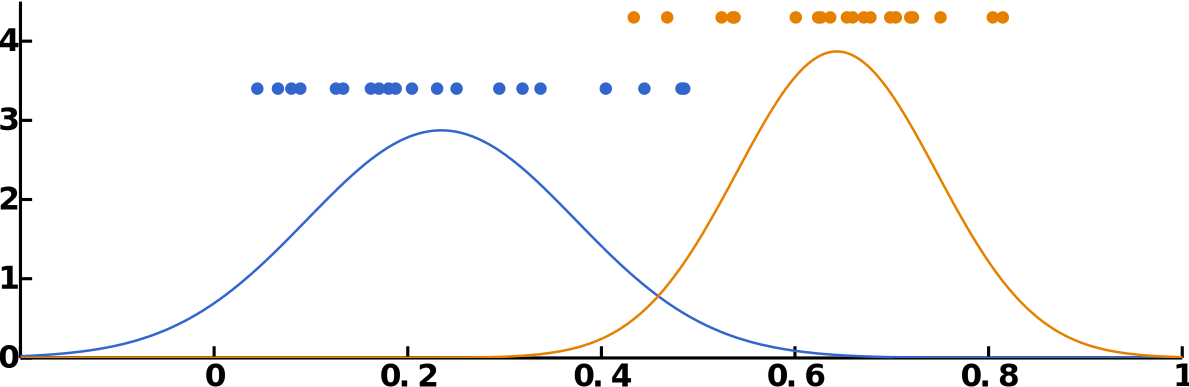
\includegraphics[width=\columnwidth]{\visualspdf/normal_diff/data.pdf}
        \caption{Normal distributions fitted from the estimated values of two hypothesis. On top are the 20 samples associated to each hypothesis. The orange distribution has a mean of 0.71 and a standard deviation of 0.17. The blue distribution has a mean of 0.23 and a standard deviation of 0.16.}
        \label{fig:normaldifferencedistribution:data}
    \end{subfigure}
    \begin{subfigure}[b]{\columnwidth}
        \centering
        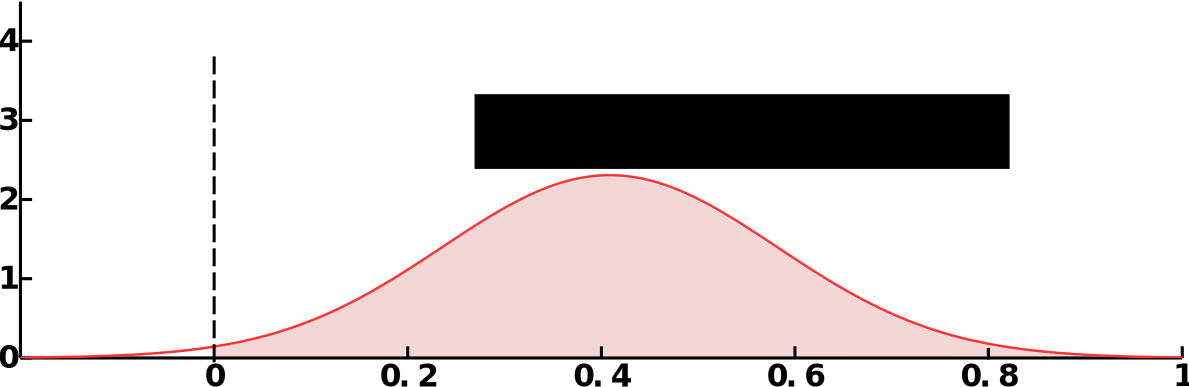
\includegraphics[width=\columnwidth]{\visualspdf/normal_diff/pdfDiff.pdf}
        \caption{Normal difference distribution between the two distribution of Figure~\ref{fig:normaldifferencedistribution:data} (the orange one minus the blue one). Mean is 0.48 and standard deviation is 0.23. From this distribution we estimate the probability that a sample has a value above zero, in this example it would be 0.99.}
        \label{fig:normaldifferencedistribution:pdf}
    \end{subfigure}
    \begin{subfigure}[b]{\columnwidth}
        \centering
        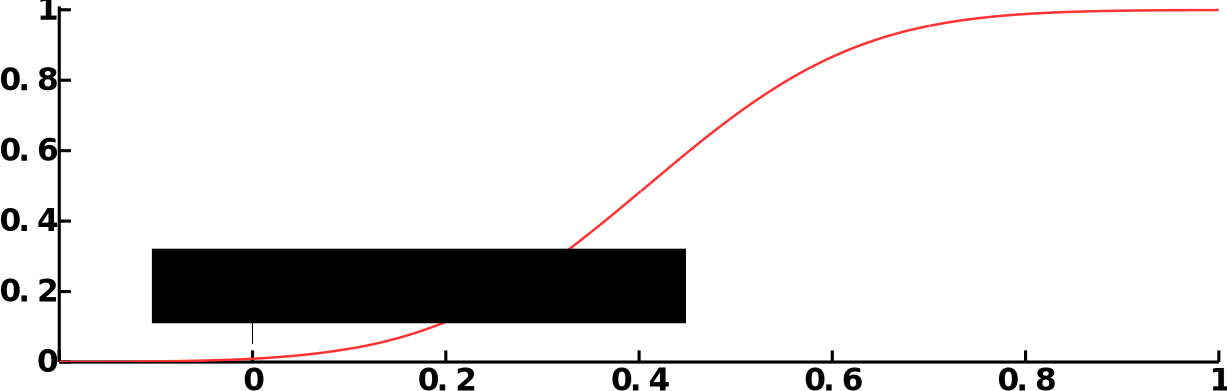
\includegraphics[width=\columnwidth]{\visualspdf/normal_diff/cdfDiff.pdf}
        \caption{Cumulative normal distribution of the Gaussian in Figure~\ref{fig:normaldifferencedistribution:pdf}.}
        \label{fig:normaldifferencedistribution:cdf}
    \end{subfigure}
\caption{The procedure used to estimate the probability that one hypothesis generates better classifiers than an other.}
\label{fig:normaldifferencedistribution}
\end{figure}

There is several weaknesses in this approach and we note that modeling a distribution on the interval [0, 1] using a normal distribution is not appropriate. Using a beta distribution would have been more suitable but we could not find an analytical solution to the difference between two beta distributions. However, we tried to use more standard statistical test, such as the one tailed Student's t-test or the Welch's t-test, but the results were not satisfying as these tests only check whether or not the means of the distributions are equals.

Note that it may seem more straightforward to directly compute the marginal probability distribution of Equation~\ref{eq:prior} which integrates over the all distribution of parameters; and use this for our likelihood estimates of Equation~\ref{eq:matchingoverfitting}. Here we tried to get a measure of confidence on top of our likelihood estimates. This is why we generate several classifiers, test their performances and measure the probability that one set of classifiers is on average better that an other set of classifiers. To do so we model the distribution of performances of a set of classifiers by a normal distribution; and compute the probability that a sample drawn from the distribution associated to one set of classifiers has higher value than one drawn from the distribution associated the an other set of classifiers.

\subsection{Selection and generation of task hypotheses}
\label{chapter:limitations:continoushypothesis:particlefilter}

As there is an infinity of possible goal states, the agent can not estimate the probability of all possible tasks in parallel. We rely on a particle filter based approach \cite{gordon1993novel,doucet2009tutorial,thrun2002particle}. The main idea consist of sampling a finite number of tasks and compute a confidence measure for each of these tasks. Given the ranking between them, we will apply a resample step which consist of keeping some of the best task and sample new ones.

There is many parameters that will influence the performance of such an algorithm. We can change the number of tasks sampled, the criteria for selecting the tasks that stay in the pool from one step to another, and we can change the method used to sample new tasks. 

As this is an exploratory experiment, we will restrict our analysis to the influence of the method used to resample the pool of task hypothesis, and consider either a random or an active strategy. We consider a pool of 50 hypothesis. Each step, we will keep only the best hypothesis from the pool and replace the 49 others using one of the sampling strategies define next.

The random generation of task simply keeps the best hypothesis and generate 49 new tasks hypothesis randomly.

Our active task generation method simply selects new tasks around the current best task hypothesis. To do so, we create a mixture of Gaussians which define the probability distribution used to sample the new tasks. This mixture model is composed of:
\begin{itemize}
\item  one fixed Gaussian at the center of the state space (i.e. $[0.5, 0.5]$), with a diagonal covariance matrix, where each value on the diagonal is equal to $0.1$, and have an associated weight of $0.2$. This Gaussian, which as a large covariance matrix relative to the state space, maintains a level of exploration in the task generation process.
\item a multitude of Gaussians, one at each location of the previous hypothesis positions (i.e. hypothesized task), whose associated weights are proportional to the probability associated to each of these tasks. The sum of the weights of these Gaussians is 0.8, such as the sum of the weights all mixture components is 1. All these Gaussians have a diagonal covariance matrix, where each value on the diagonal is equal to $0.01$. For computational purpose, each Gaussian had a minimal weight of $1e^{-6}$.
\end{itemize}
Note that the resulting distribution will be truncated as all the point generated outside of the boundaries of the space (i.e. between 0 and 1 for each dimension) will be shifted to the closest position in the state space.

\subsection{Uncertainty based state sampling}

The agent can also control the next state to teleport to. As seen in chapter~\ref{chapter:planning}, actively controlling agent states can lead to better performances. Indeed the state of the agent influences the signal sent by the teacher. 

We will compare two kinds of sampling, random and an uncertainty based method. The random method simply teleport the agent to a random position in the world. The active method rely again on a sampling method. At each step, we generate 1000 states randomly and compute the uncertainty associated to these states using the method described in chapter~\ref{chapter:planning} by Equation~\ref{eq:planning} and using up to 20 sampled signals from our history of interaction. To chose the next state, we select, among the 1000 points, the state that as higher uncertainty, and teleport the agent to that state in order to collect the next teaching signal.

\subsection{Results}

We compare all four combinations of the methods described above \begin{inparaenum}[a)] \item random state and task selection (which we call ``random random''), \item random selection of next state and active task sampling (which we call ``random active''), \item uncertainty based selection of next state and random task selection (which we call ``uncertainty random''), and \item uncertainty based selection of next state and active task sampling (which we call ``uncertainty active''). \end{inparaenum}

We ran 100 simulated experiments for each method and each dataset. Each experiment lasted 200 iterations and started by 12 random steps such as to collect enough signals to use Equation~\ref{eq:jeffreysmean}~and~\ref{eq:jeffreyscov} with our 11 dimensional signals.

\paragraph{Distance to goal state}

We first analyze the results using the directional finger movement dataset shown in Figure~\ref{fig:fingerdatasetdirection}. For each method, we compare the evolution of the distance between the best task hypothesis through iteration (the more probable according to our estimate) and the goal state (see Figure~\ref{fig:continuoustaskdistevolution}).

Only the combination of actively sampling new tasks and actively selecting new states based on their uncertainty as overall better performance than any other combination of methods. These two methods are complementary, our active task sampling method allows to explore close to our previous best estimates, and our uncertainty based state selection allow to sample state in very precise location to be able to differentiate between close hypothesis. It also explains why using one of the active methods in alone does not reach the same performances.

\begin{figure}[!htbp]
\centering
\includegraphics[width=0.62\columnwidth]{\imgpath/continuous_task/distEvolution.eps}
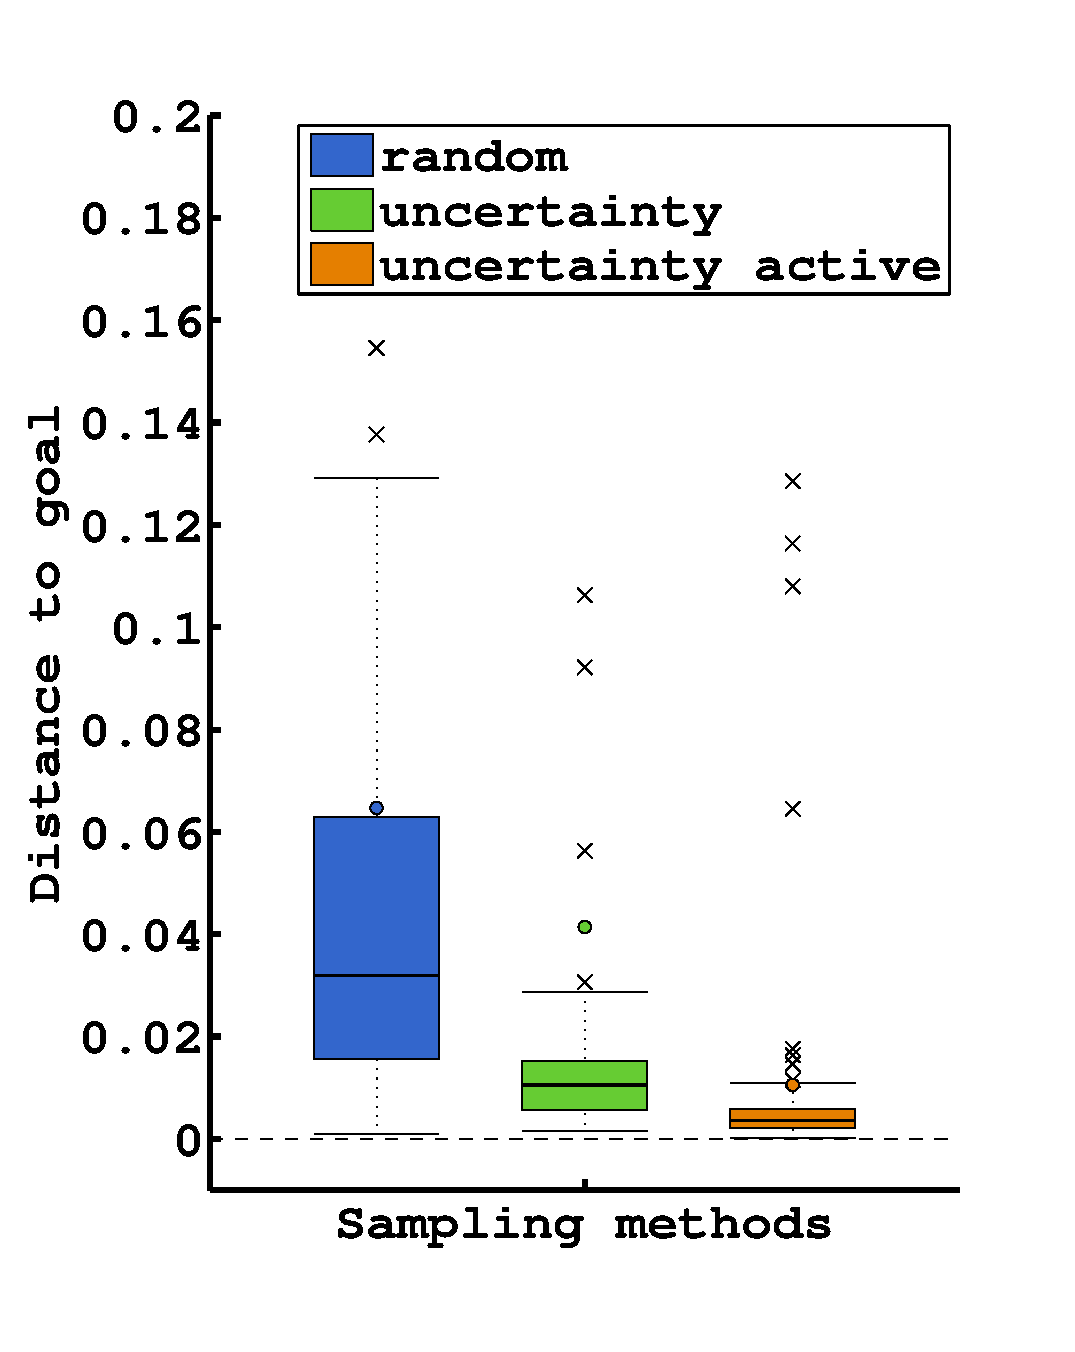
\includegraphics[width=0.37\columnwidth]{\imgpath/continuous_task/endDist.eps}
\caption{Evolution of the distance to the target using the directional finger movement dataset shown in Figure~\ref{fig:fingerdatasetdirection}. On the left is the evolution of the distance of the best position hypothesis to the goal position (mean and standard error shown as shaded area). On the right is a box plot of the distance of the best position hypothesis to the goal position at the end of the 200 iterations. Actively sampling new task hypothesis as well as selecting new state based on our uncertainty estimation outperform allow to identify the target position with very high accuracy and low variance. We note that some distant outliers are not shown on the box plots for readability reasons.}
\label{fig:continuoustaskdistevolution}
\end{figure}

In Figure~\ref{fig:continuoustaskdistevolution} (right), we compare the distribution of final distance between our best hypothesis and the true goal position. First note that the important difference between displaying our results in terms of mean and standard error or in terms of a box plot, which shows the median and the 25th and 75th percentile (you can see the mean value as a colored dot). Especially for the ``uncertainty random'' method, the visual impression of the performance of the methods differs. This is due to the outliers, where even a few values far away from the main group of point can ``push'' the mean away. The normal distribution assumption do not hold for presenting our results. 

Therefore, in order to statistically compare the efficiency of our methods, we use the Mann-Whitney U-test \cite{mann1947test} which is a nonparametric test for equality of population medians of two independent samples. We use the one tailed version to specifically test whether one population has greater performances than the other. There is no measurable statistical difference between the ``random random'' and ``random active'' methods ($p = 0.68$). The ``uncertainty random'' performances over ``random random'' ($p<1e^{-10}$) and ``random active'' ($p<1e^{-10}$) are highly significant. As well as the difference between the ``uncertainty active'' and ``uncertainty random'' difference in performance ($p<1e^{-10}$).

The results presented above were obtained using the directional finger movement dataset shown in Figure~\ref{fig:fingerdatasetdirection}. We now demonstrated how the same algorithm could handle different user finger gestures. To do so we repeat the experiment with the cardinal sign dataset of Figure~\ref{fig:fingerdatasetsigns}.

\begin{figure}[!htbp]
\centering
\includegraphics[width=0.62\columnwidth]{\imgpath/continuous_task/distEvo_signs.eps}
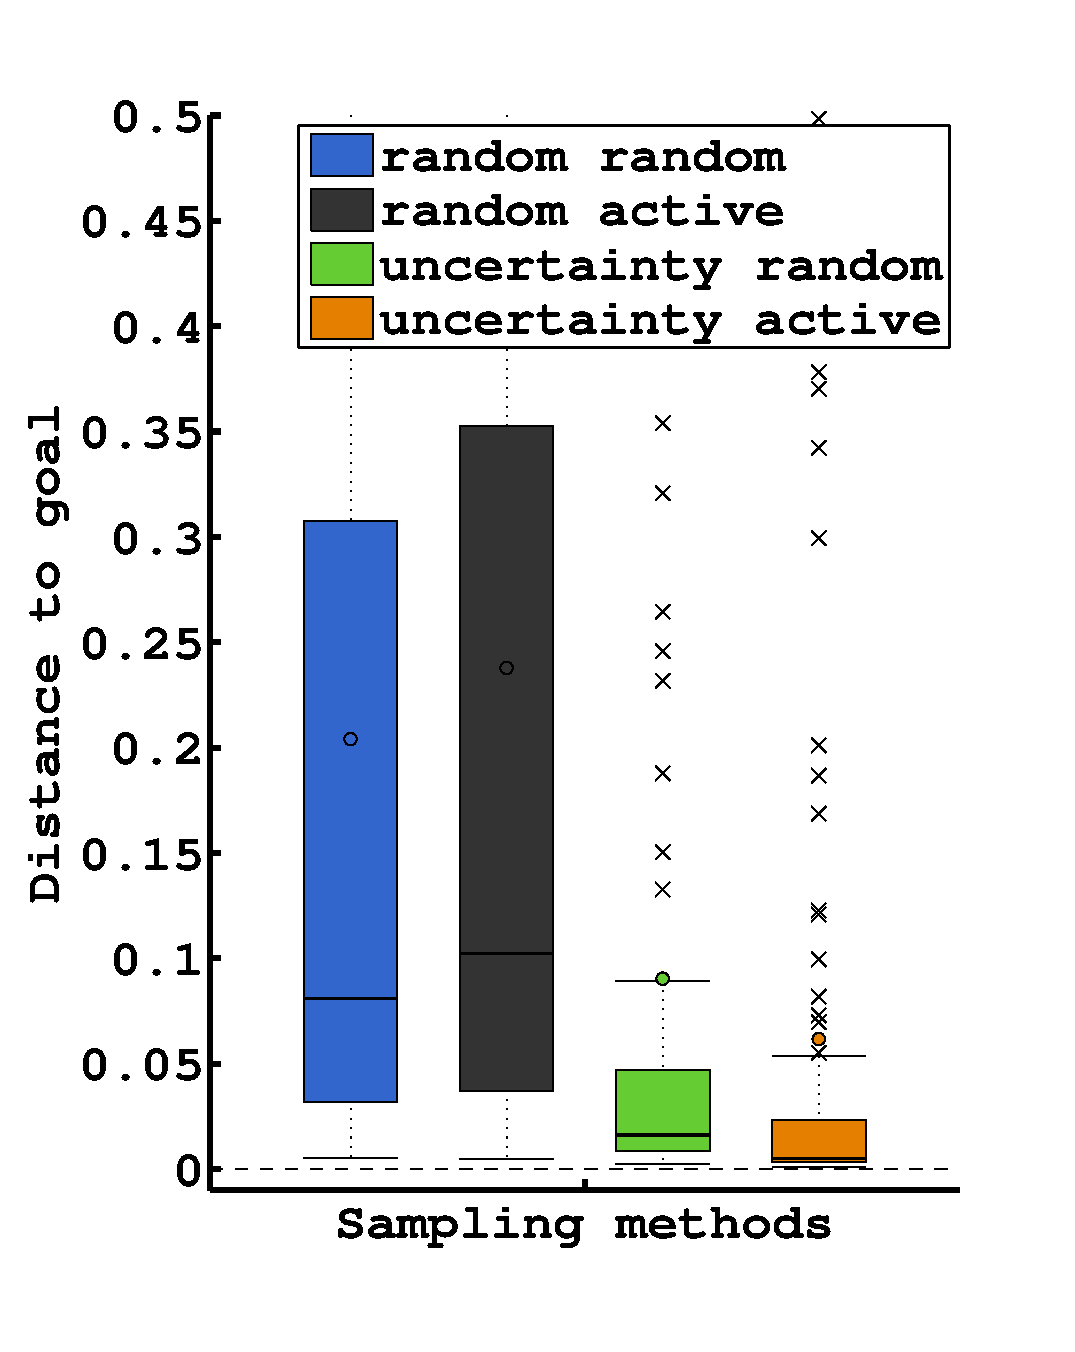
\includegraphics[width=0.37\columnwidth]{\imgpath/continuous_task/endDist_signs.eps}
\caption{Evolution of the distance to target using the cardinal signs finger movement dataset shown in Figure~\ref{fig:fingerdatasetsigns}. On the left is the evolution of the distance of the best position hypothesis to the goal position (mean and standard error shown as shaded area). On the right is a box plot of the distance of the best position hypothesis to the goal position at the end of the 200 iterations. Actively sampling new task hypothesis as well as selecting new state based on our uncertainty estimation outperform allow to identify the target position with very high accuracy and low variance. We note that some distant outliers are not shown on the box plots for readability reasons.}
\label{fig:continuoustaskdistevolution_signs}
\end{figure}

Figure~\ref{fig:continuoustaskdistevolution_signs} (left) shows the evolution of the distance between the best task estimates and the goal task. We observe a larger difference between random and uncertainty based selection of next state. This could be explained by the properties of the cardinal sign dataset, where the system must consider all features to differentiate between classes, therefore requiring more signals to be collected. For the directional finger movement dataset (Figure~\ref{fig:fingerdatasetdirection}), only two features (end position on X and Y axis) were enough to differentiate between all classes.

In Figure~\ref{fig:continuoustaskdistevolution_signs} (right), we compare the distribution of final distance between our best hypothesis and the true goal position. There is no measurable statistical difference between the ``random random'' and ``random active'' methods ($p = 0.8687$). The ``uncertainty random'' performances over ``random random'' ($p<1e^{-10}$) and ``random active'' ($p<1e^{-10}$) are highly significant. As well as the difference between the ``uncertainty active'' and ``uncertainty random'' difference in performance ($p<1e^{-5}$).

Finally, we note that the final median distance between the best position estimation and the goal position are 0.0036 and 0.0051 for the directional movement and cardinal sign movement respectively. 
% While this does not really matter, this difference is significant ($p< 1e^{-3}$). 
It is important to project this results in the real word, it means that given a one meter square area, our agent is able to find the position the user has in mind with less that 5 millimeters ( half of the time and given 200 requests), but without knowing the signal to meaning mapping beforehand. Moreover, as we have seen with our two datasets (Figure~\ref{fig:fingerdatasetdirection} and Figure~\ref{fig:fingerdatasetsigns}), given our simple representation of the finger movements, a great variety of possible signals can be considered.

\paragraph{Task sampling comparison}

We briefly illustrate the difference between our two task sampling methods, namely ``random'' and ``active''.

Figure~\ref{fig:continuoustasktasksampling} shows the task sampled (in blue) at steps 15, 50, and 150 following a random (Fig.~\ref{fig:continuoustaskrandomtask}) or an active (Fig.~\ref{fig:continuoustaskactivetask}) resampling step. The active resampling allows to focus the set of task around the goal state (in red), which increases the changes of finding a better estimates of the task.

\begin{figure}[!htbp]
\centering
    \begin{subfigure}[b]{\columnwidth}
        \centering
        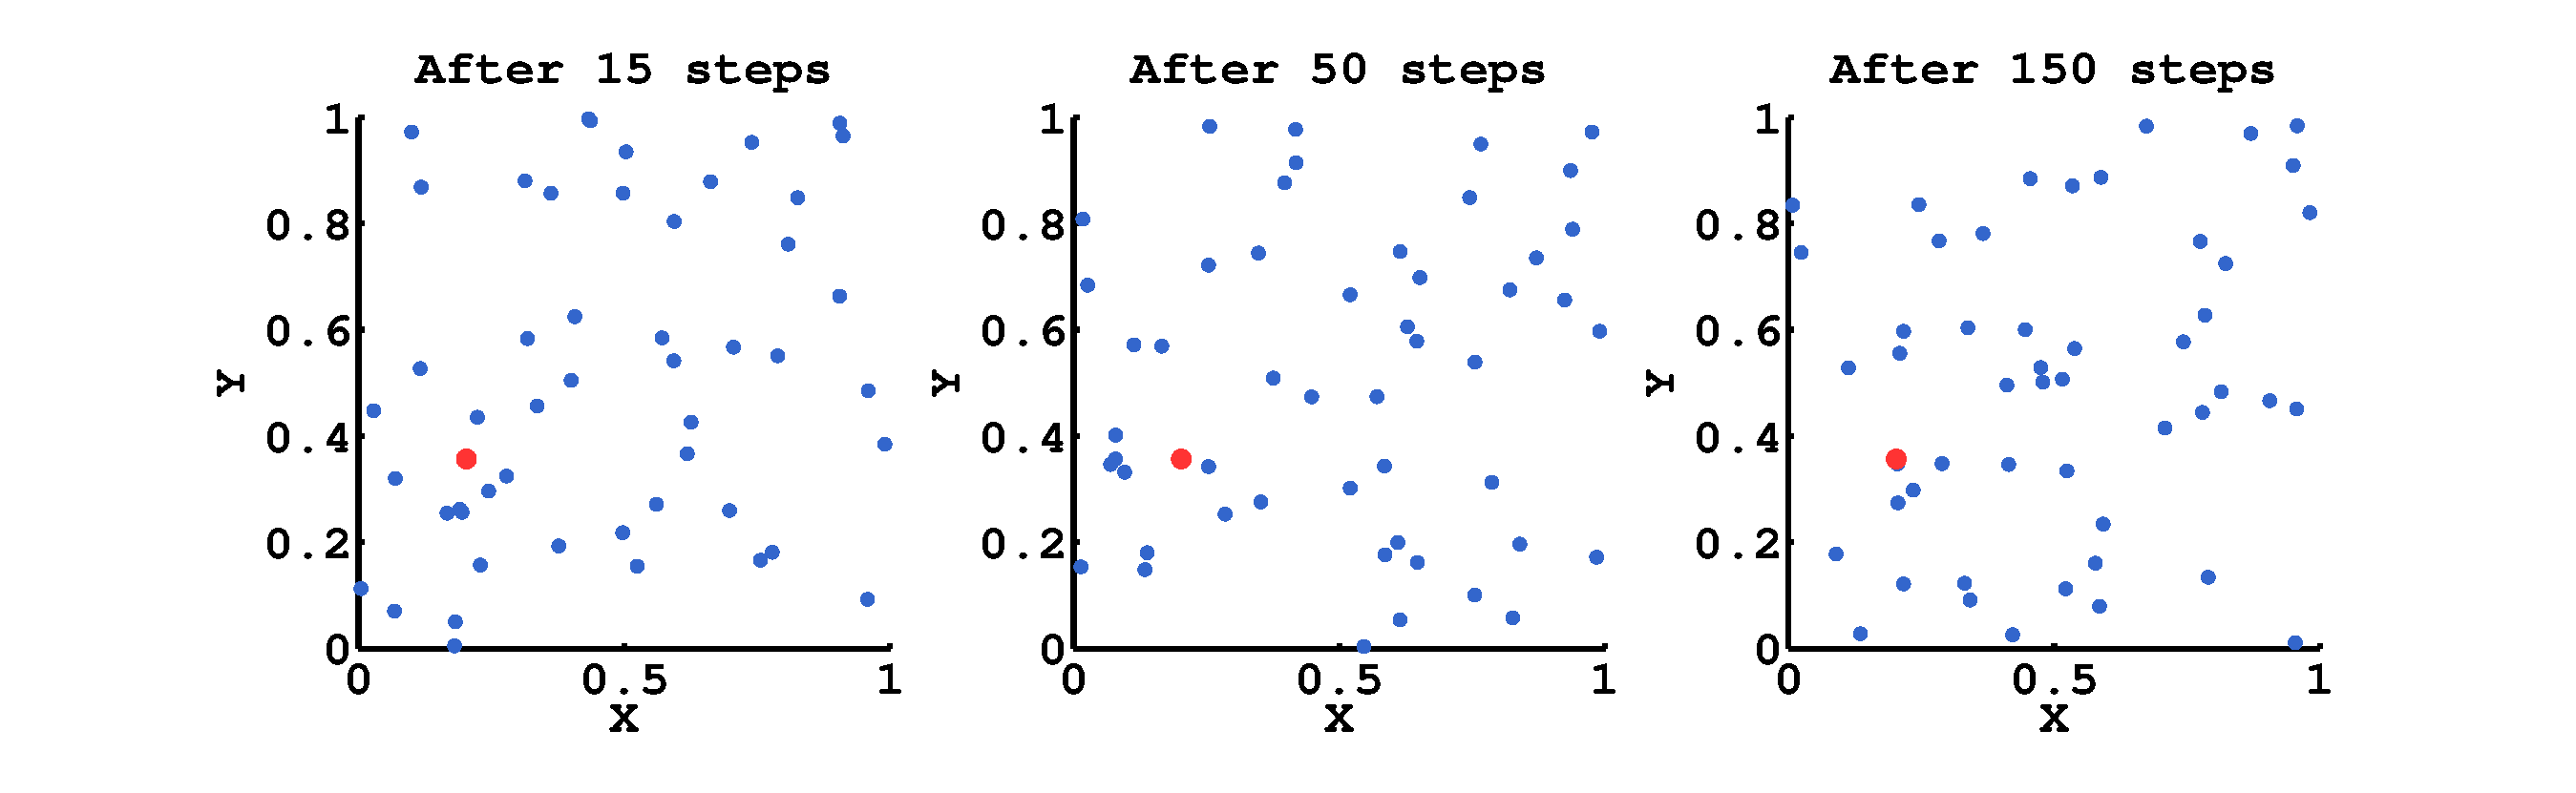
\includegraphics[width=\columnwidth, trim=3.5cm 0cm 3.5cm 0cm, clip=true]{\imgpath/continuous_task/maps/random_task_sampling.eps}
        \caption{Example of task hypothesis sampled using a random method.}
        \label{fig:continuoustaskrandomtask}
    \end{subfigure}
    \begin{subfigure}[b]{\columnwidth}
        \centering
        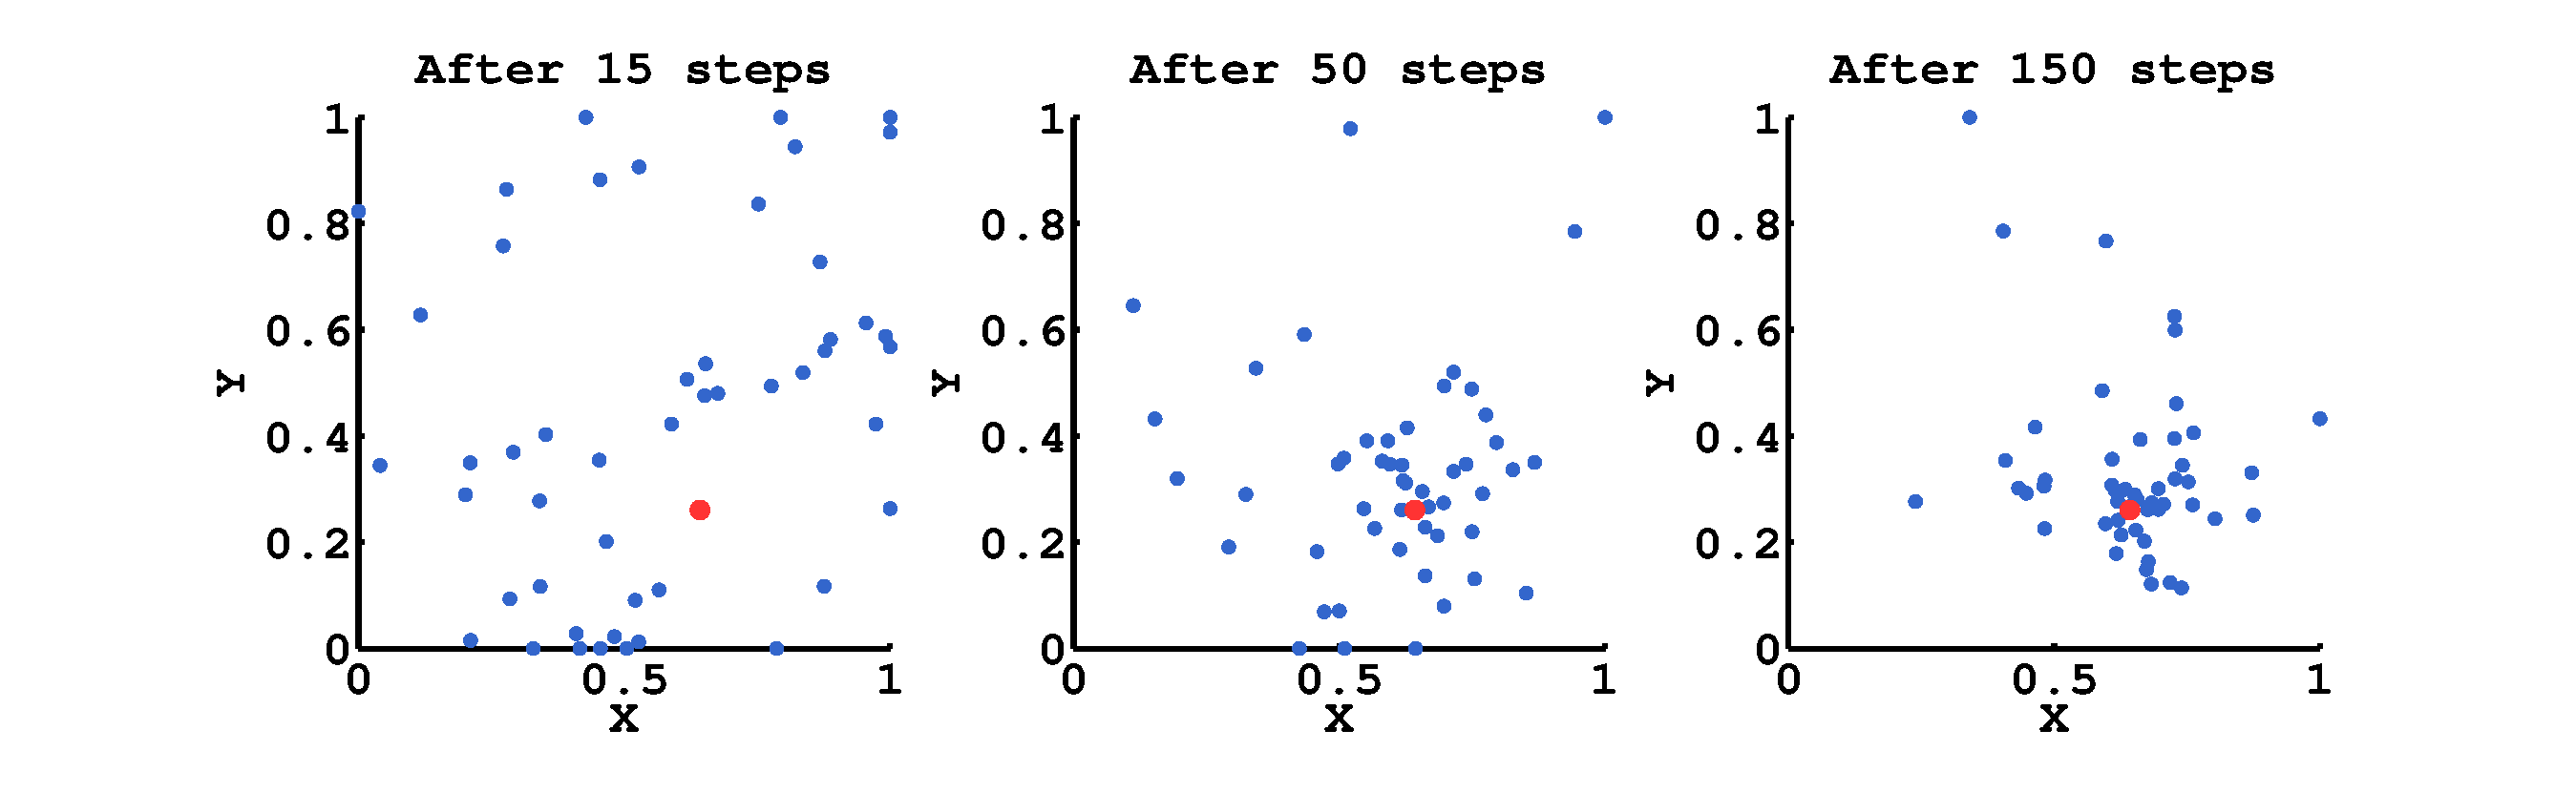
\includegraphics[width=\columnwidth, trim=3.5cm 0cm 3.5cm -1cm, clip=true]{\imgpath/continuous_task/maps/active_task_sampling.eps}
        \caption{Example of task hypothesis sampled using our active method.}
        \label{fig:continuoustaskactivetask}
    \end{subfigure}
\caption{Examples of task hypothesis sampling strategies. In red is the goal task. In blue are the sampled task hypothesis at iteration 15, 50 and 150. The active sampling method progressively focus his sampling around the goal state.}
\label{fig:continuoustasktasksampling}
\end{figure}

\newpage

\paragraph{State sampling comparison}

We briefly illustrate the difference between our two state sampling methods, namely ``random'' and ``uncertainty''.

Figure~\ref{fig:continuoustaskstatesampling} shows the state visited (in blue) at after 200 steps  following a random (Fig.~\ref{fig:continuousstaterandomstates}) or an uncertainty based (Fig.~\ref{fig:continuousstateuncertaintystates}) next state selection method. The uncertainty based method allows to visit more states around the goal state (in red).

 % which increases the changes of differentiates between the set of task hypothesis.

\begin{figure}[!htbp]
\centering
    \begin{subfigure}[t]{0.49\columnwidth}
        \centering
        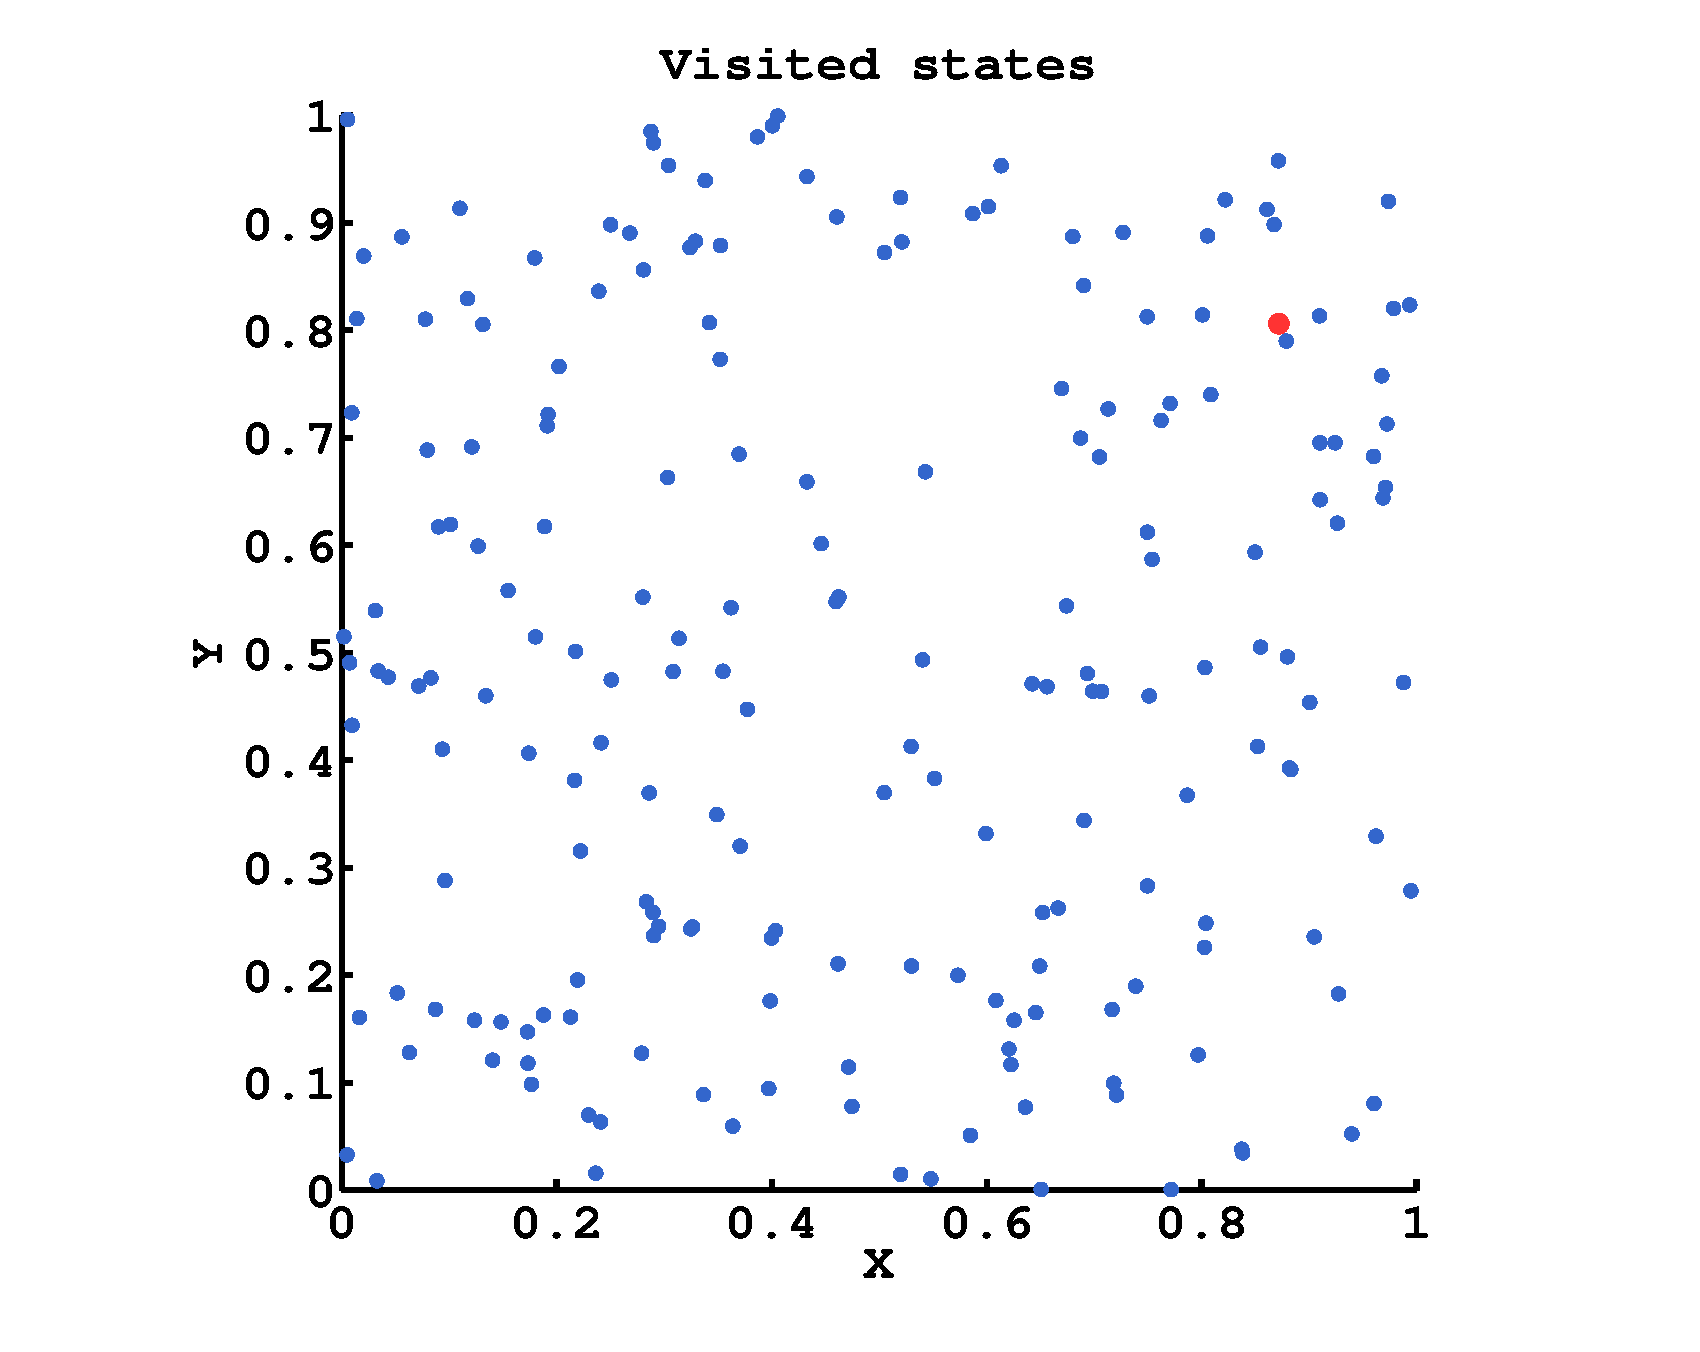
\includegraphics[width=\columnwidth, trim=2.5cm 0cm 2.5cm 0cm, clip=true]{\imgpath/continuous_task/maps/random_state_sampling.eps}
        \caption{Visited states after 200 steps with random state selection.}
        \label{fig:continuousstaterandomstates}
    \end{subfigure}
    \begin{subfigure}[t]{0.49\columnwidth}
        \centering
        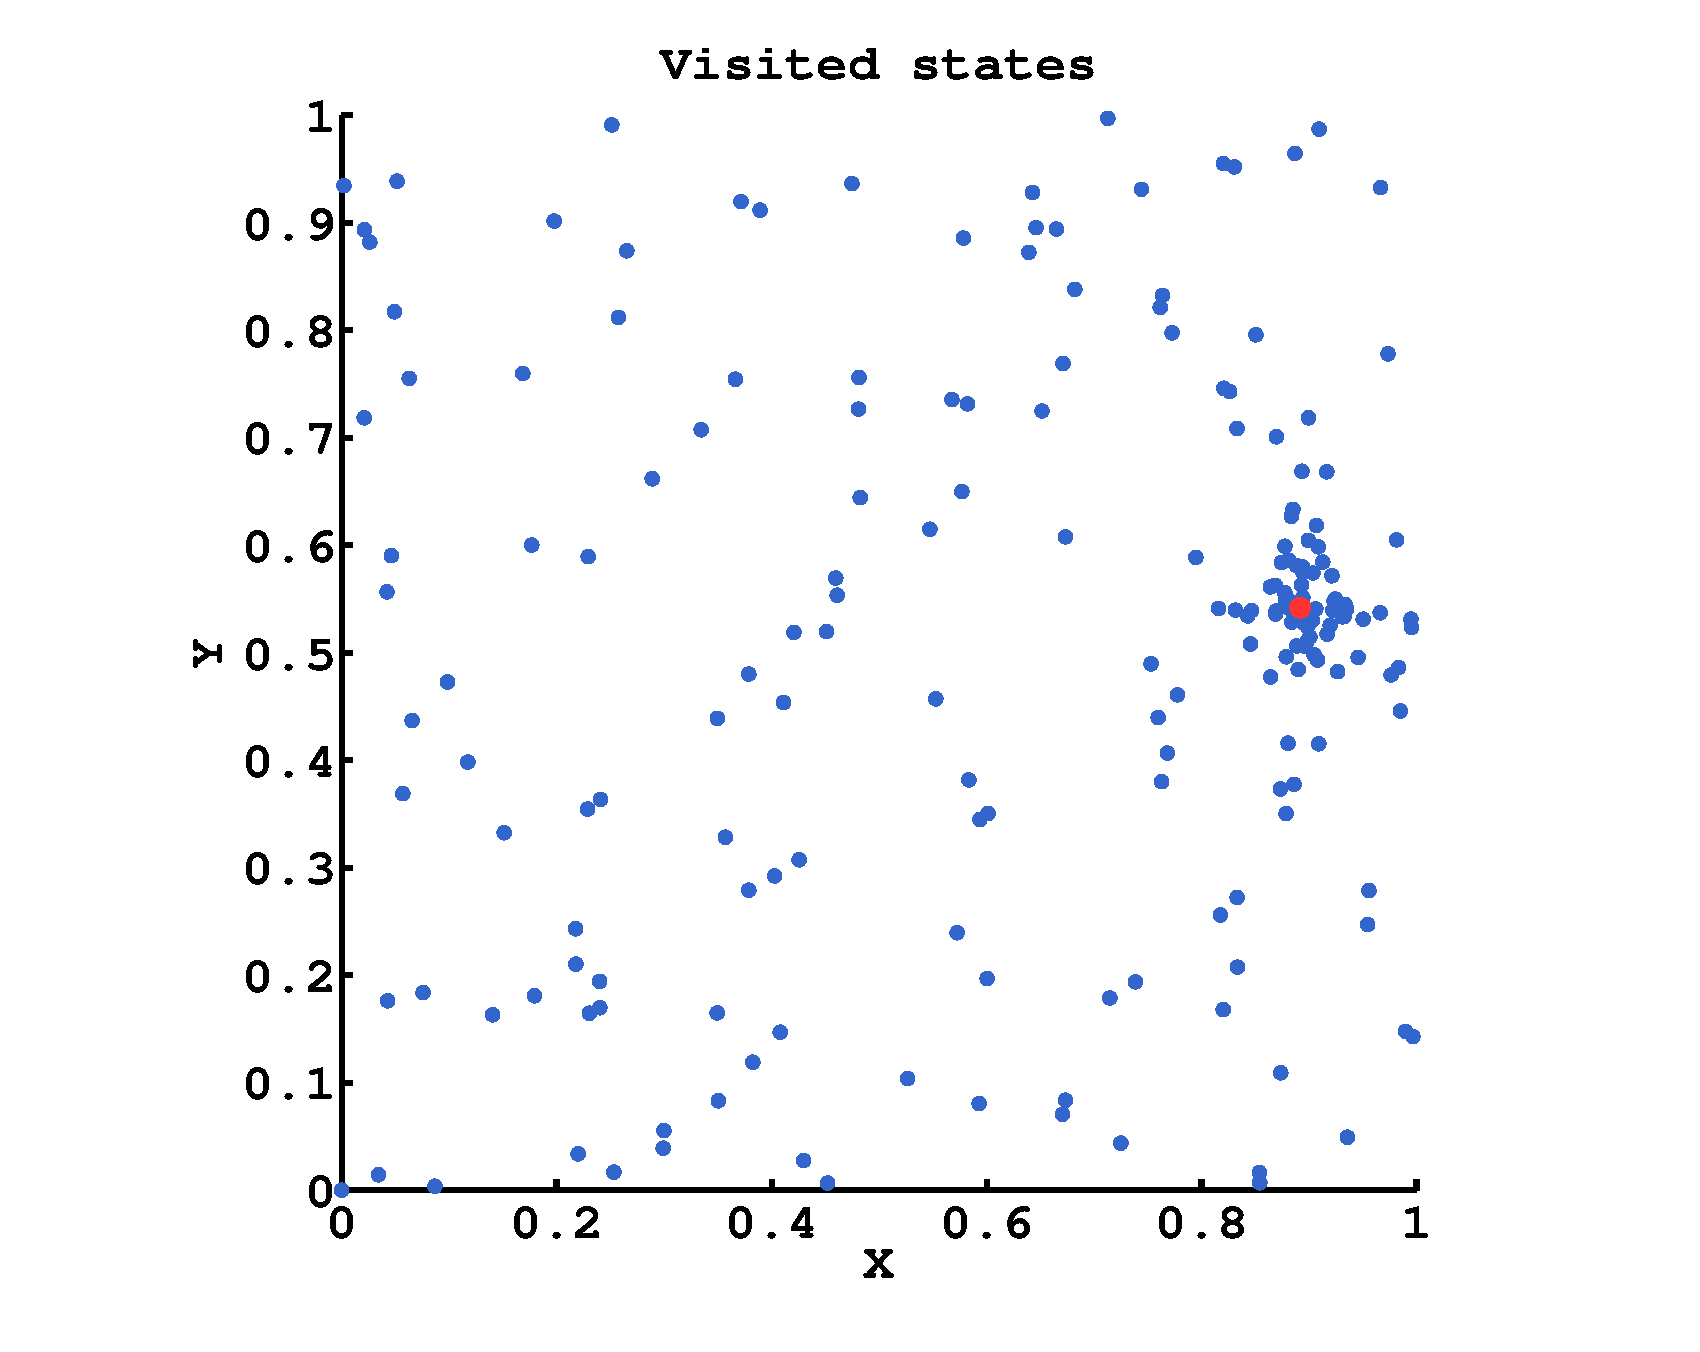
\includegraphics[width=\columnwidth, trim=2.5cm 0cm 2.5cm 0cm, clip=true]{\imgpath/continuous_task/maps/uncertainty_state_sampling.eps}
        \caption{Visited states after 200 steps with uncertainty based state selection.}
        \label{fig:continuousstateuncertaintystates}
    \end{subfigure}
\caption{The state visited by the agent, i.e. in which it received instruction signals, after 200 steps. In red is the goal task. Comparison of random state selection (left) and uncertainty based state selection (right). Selecting state according to their uncertainty, allow to collect more information around the goal state, which allow to identify more precisely the target location.}
\label{fig:continuoustaskstatesampling}
\end{figure}

Figure~\ref{fig:continuoustasktasksamplingexampleslow} details the uncertainty based method for selecting the next visited states. Figure~\ref{fig:continuoustaskexampleslowdist} present the goal state for this specific run (right) and the evolution of the distance to the goal of the best estimate (left). Figure~\ref{fig:continuoustaskexampleslowweights} shows the set of task hypothesis at steps 15, 50, and 150 (as for Figure~\ref{fig:continuoustasktasksampling}) where the colors associated to each point represent the estimated probability of each task (red is high, blue is low). To sample the following agent's state, we sample 1000 states randomly and estimates the uncertainty of each of those point using the method described in chapter~\ref{chapter:planning} by Equation~\ref{eq:planning}. Computing this uncertainty requires to have a set of hypothesis and their associated weights (shown in Figure~\ref{fig:continuoustaskexampleslowweights}), access to the interaction frame, and to a classifier for each hypothesis. The resulting maps for step 15, 50, and 150 are displayed in Figure~\ref{fig:continuoustaskexampleslowuncertainty} where the colors represent the uncertainty values (red is high, blue is low). The less the distribution of probably on task is flat, the more the uncertainty map is narrow and focused around the best estimate. The active task resampling step is beneficial to the uncertainty state selection step as it allows to specify the uncertainty in key areas.

\begin{figure}[!p]
\centering
    \begin{subfigure}[b]{\columnwidth}
        \centering
        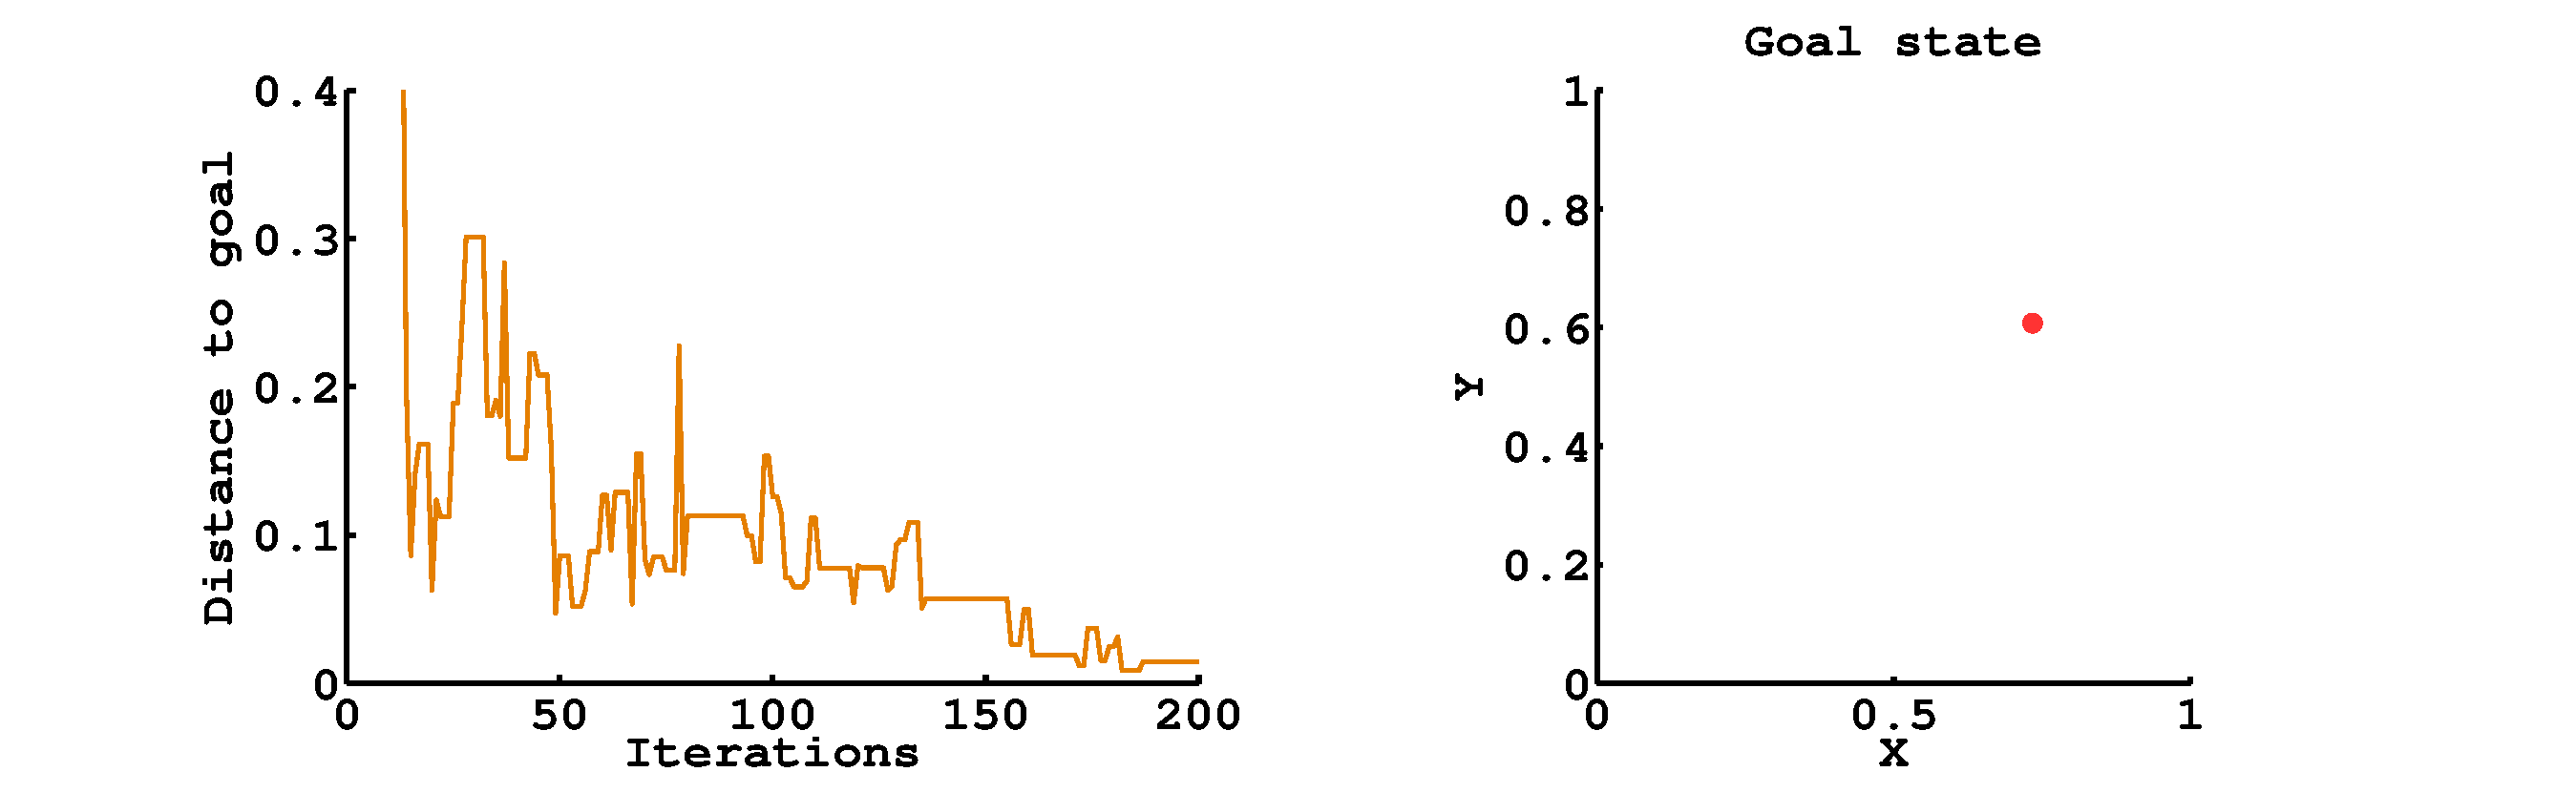
\includegraphics[width=\columnwidth]{\imgpath/continuous_task/maps/distgoal_slow.eps}
        \caption{Evolution of distance between the best estimate and the goal position (left). The goal position being the red dot on the right plot.}
        \label{fig:continuoustaskexampleslowdist}
    \end{subfigure}
    \begin{subfigure}[b]{\columnwidth}
        \centering
        \includegraphics[width=0.95\columnwidth, trim=2.5cm 0cm 2.5cm -1cm, clip=true]{\imgpath/continuous_task/maps/weights_slow.eps}
        \caption{Set of hypothesis after 15, 50, and 150 steps, with their associated probability show as colors. The associated value to each color are different for each time step. Red is associated to the most probable task, and blue for the less probable. The colors linearly maps according to their associated weights, red (blue) for the most (less) probable task.}
        \label{fig:continuoustaskexampleslowweights}
    \end{subfigure}
    \begin{subfigure}[b]{\columnwidth}
        \centering
        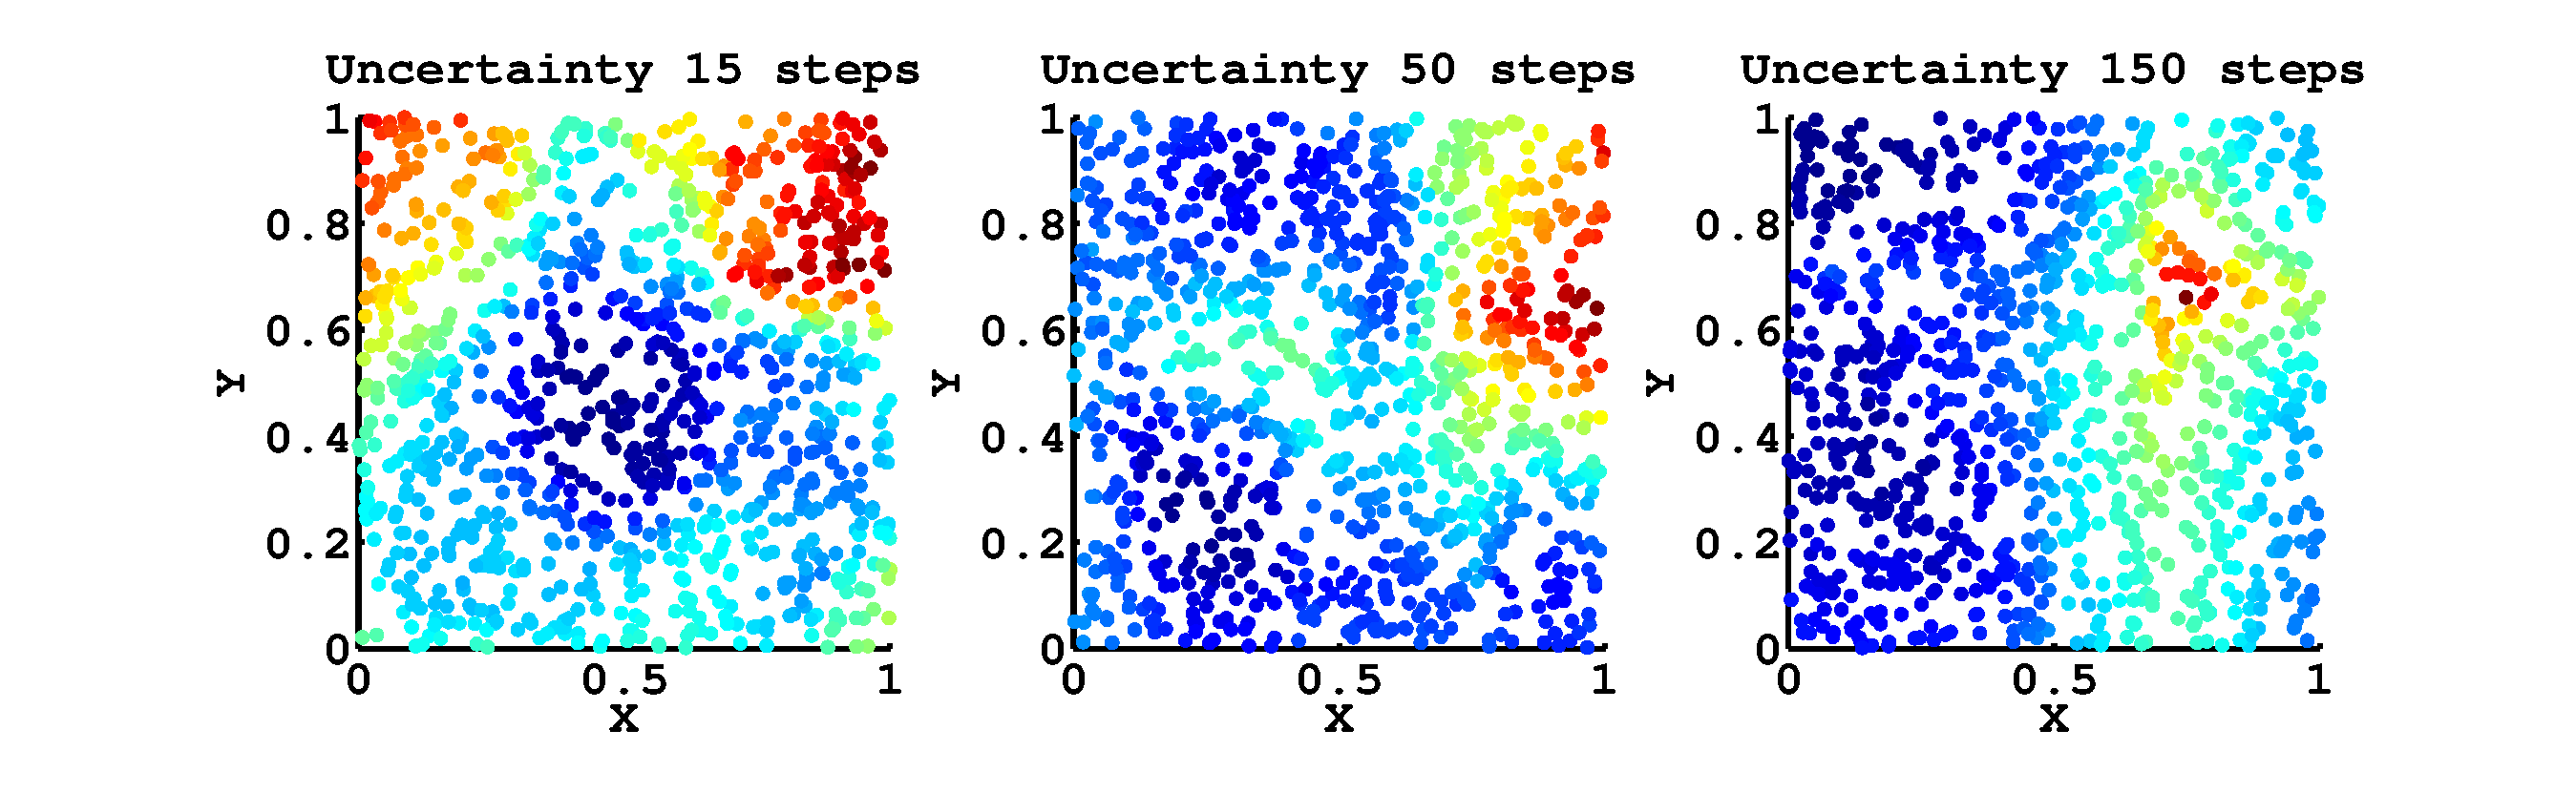
\includegraphics[width=0.95\columnwidth, trim=2.5cm 0cm 2.5cm -1cm, clip=true]{\imgpath/continuous_task/maps/uncertainty_slow.eps}
        \caption{Uncertainty associated to each of the 1000 sampled states after 15, 50, and 150 steps. The most uncertain state will be selected as the next state of the agent. The uncertainty maps evolve through time as the set of task hypothesis and their respective probabilities are updated. After 150 steps, the uncertainty is located around the goal position. The colors linearly maps according to their associated weights, red (blue) for the most (less) probable task.}
        \label{fig:continuoustaskexampleslowuncertainty}
    \end{subfigure}
\caption{Illustration of the uncertainty based state sampling process after 15, 50, and 150 steps. The uncertainty is evaluated for 1000 randomly generated states according to the current set of task hypothesis and their associated probabilities.}
\label{fig:continuoustasktasksamplingexampleslow}
\end{figure}

% \section{Discussion}

% In this section we have seen that it is possible to remove the
%!TEX root = ../../thesis.tex

\section{Interaction frame hypothesis}
\label{chapter:limitations:framehypothesis}

\question{How to leverage from the pre-defined unique interaction frame?}

Until now we have assumed that the interaction frame, which specifies the details of the interaction between the human and the machine was known. In this frame only the meaning of the signal was unknown. We now open this side of the interaction and considered the case where multiple interaction are define, but only one of them account for the interaction between the human and the machine.

\subsection{Illustrations}

We will use a very simple example to illustrate the problem and show computational results on the same simple scenario. We consider that the agent lives in the line word as defined in chapter~\ref{chapter:lfui::symmetries}, where the agent has access to the ``no move'' action in order to remove the symmetry problem. The agent knowns it should reach either of the two edges of the world, G1 or G2. And the agent knowns that the teacher is providing either feedback or guidance instructions. To handle this new hidden information we will rely again on our interpretation hypothesis process. This time, one hypothesis will be the combination of one task hypothesis and one frame hypothesis.  For our simple example, it results in having four hypothesis.

The result of the labeling process is shown in Figure~\ref{fig:multipleframeexplainedfeedback} for a teacher providing feedback instruction according the task G1 (of course the agent do not have access to this information). The hypothesis that labels the signals according to the task G1 and the feedback frame is the one whose signal-labels pair match better with he underlying structure of the data. Indeed for the guidance case, the labeling process for hypothesis G1 is always giving a ``left'' label whether or not the agent is moving away or closer to the target which allow to differentiate between feedback and guidance case. To differentiate between G1 and G2, the same principle than the one described in chapter~\ref{chapter:lfui::symmetries} applies.

\begin{figure}[!ht]
\centering
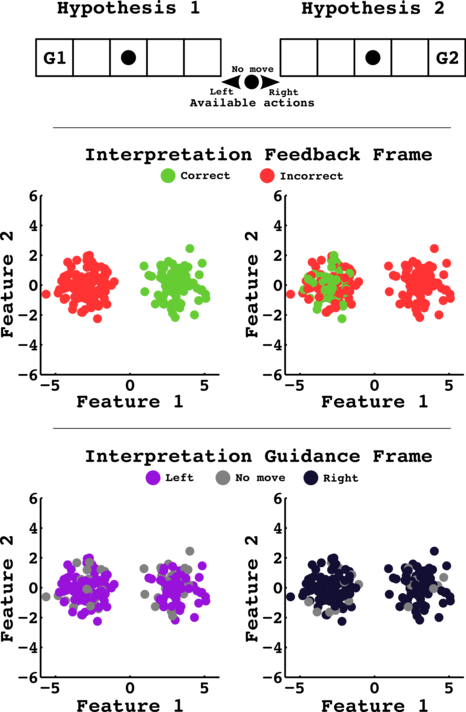
\includegraphics[width=\twoplanningwidth\columnwidth]{\visualspdf/multiple_frame/multiple_frame_feedback.pdf}
\caption{Illustration of the labelling porcess on both task and interaction frame hypothesis. The agent can perform right, left, or a ``no move'' action. The agent receive feedback on its action in the line word according to G1 . The agent do not known which task (G1 or G2) neither which interaction scheme the teacher is following (feedback or guidance). The result of the labeling process allow to identify the hypothesis on task G1 and feedback frame as the more likely.}
\label{fig:multipleframeexplainedfeedback}
\end{figure} 

Considering now that the teacher is providing guidance instruction according the task G1, the results of the labeling process can be seen in Figure~\ref{fig:multipleframeexplainedguidance}. The same explanation than for Figure~\ref{fig:multipleframeexplainedfeedback} applies. 

\begin{figure}[!ht]
\centering
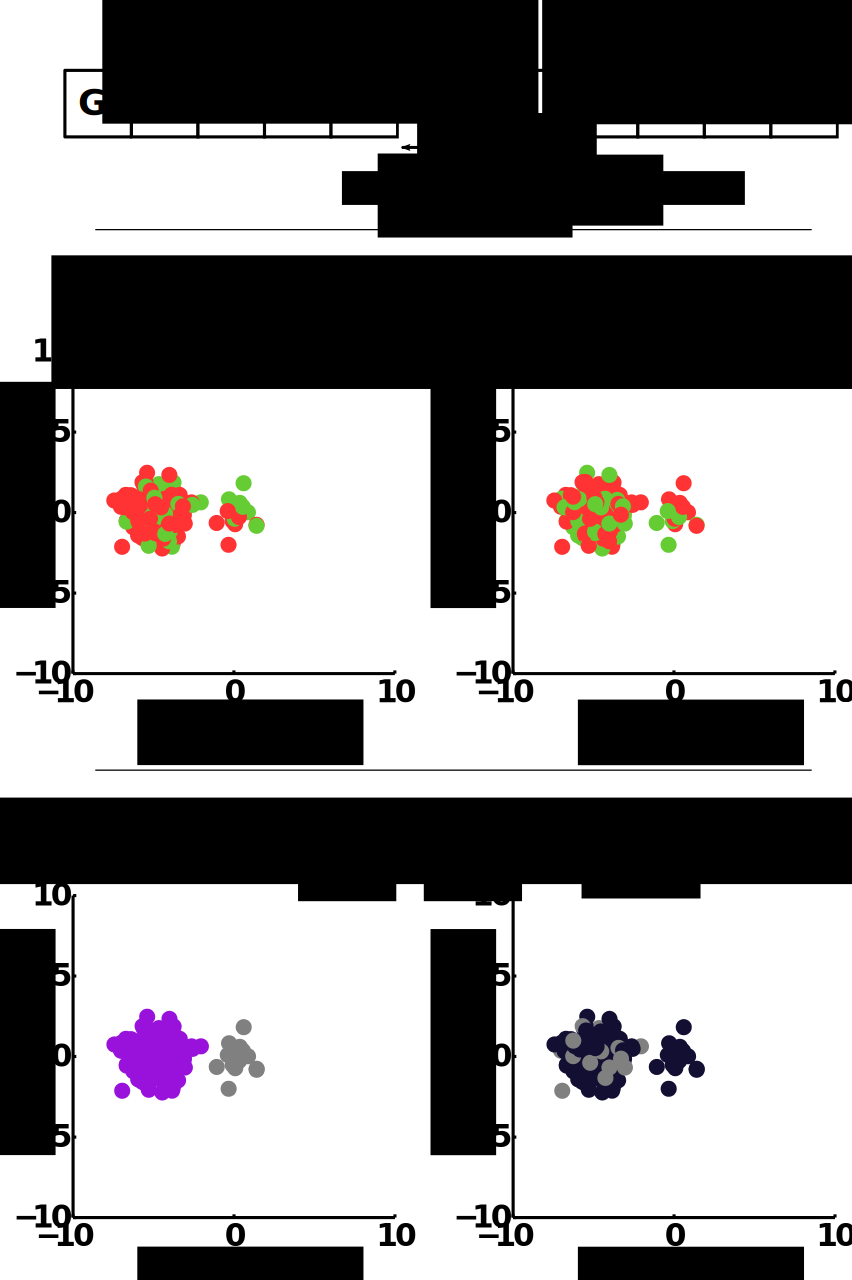
\includegraphics[width=\twoplanningwidth\columnwidth]{\visualspdf/multiple_frame/multiple_frame_guidance.pdf}
\caption{Illustration of the labelling porcess on both task and interaction frame hypothesis. The agent can perform right, left, or a ``no move'' action. The agent receive guidance instruction on its action in the line word according to G1 . The agent do not known which task (G1 or G2) neither which interaction scheme the teacher is following (feedback or guidance). The result of the labeling process allow to identify the hypothesis on task G1 and guidance frame as the more likely.}
\label{fig:multipleframeexplainedguidance}
\end{figure} 

\subsection{Simple experiments}

We now verify that the algorithm works in practice. We consider the same line world scenario as described above. For our experiments, the simulated teacher select randomly a target (G1 or G2) and an interaction frame (feedback or guidance). The agent is using our uncertainty based planning method as well as the same setting as described in chapter~\ref{chapter:planning:method}. We ran 100 simulations

Figure~\ref{fig:multipleframeall} shows the evolution of our probability measure of the correct combination of task and interaction frame, which is adapted from Equation~\ref{eq:probapairwise} in chapter~\ref{chapter:lfui:confidence} (minimum of pairwise normalized likelihood) where each hypothesis is a combination of task and interaction frame. After 200 steps, all our experiments identified with probability 1 the correct combination of task and interaction frame. In practice, in our previous experiments, we used a confidence threshold of 0.9, under this condition most of our experiments would have identified the task in slighlty more than 50 steps.

\begin{figure}[!ht]
\centering
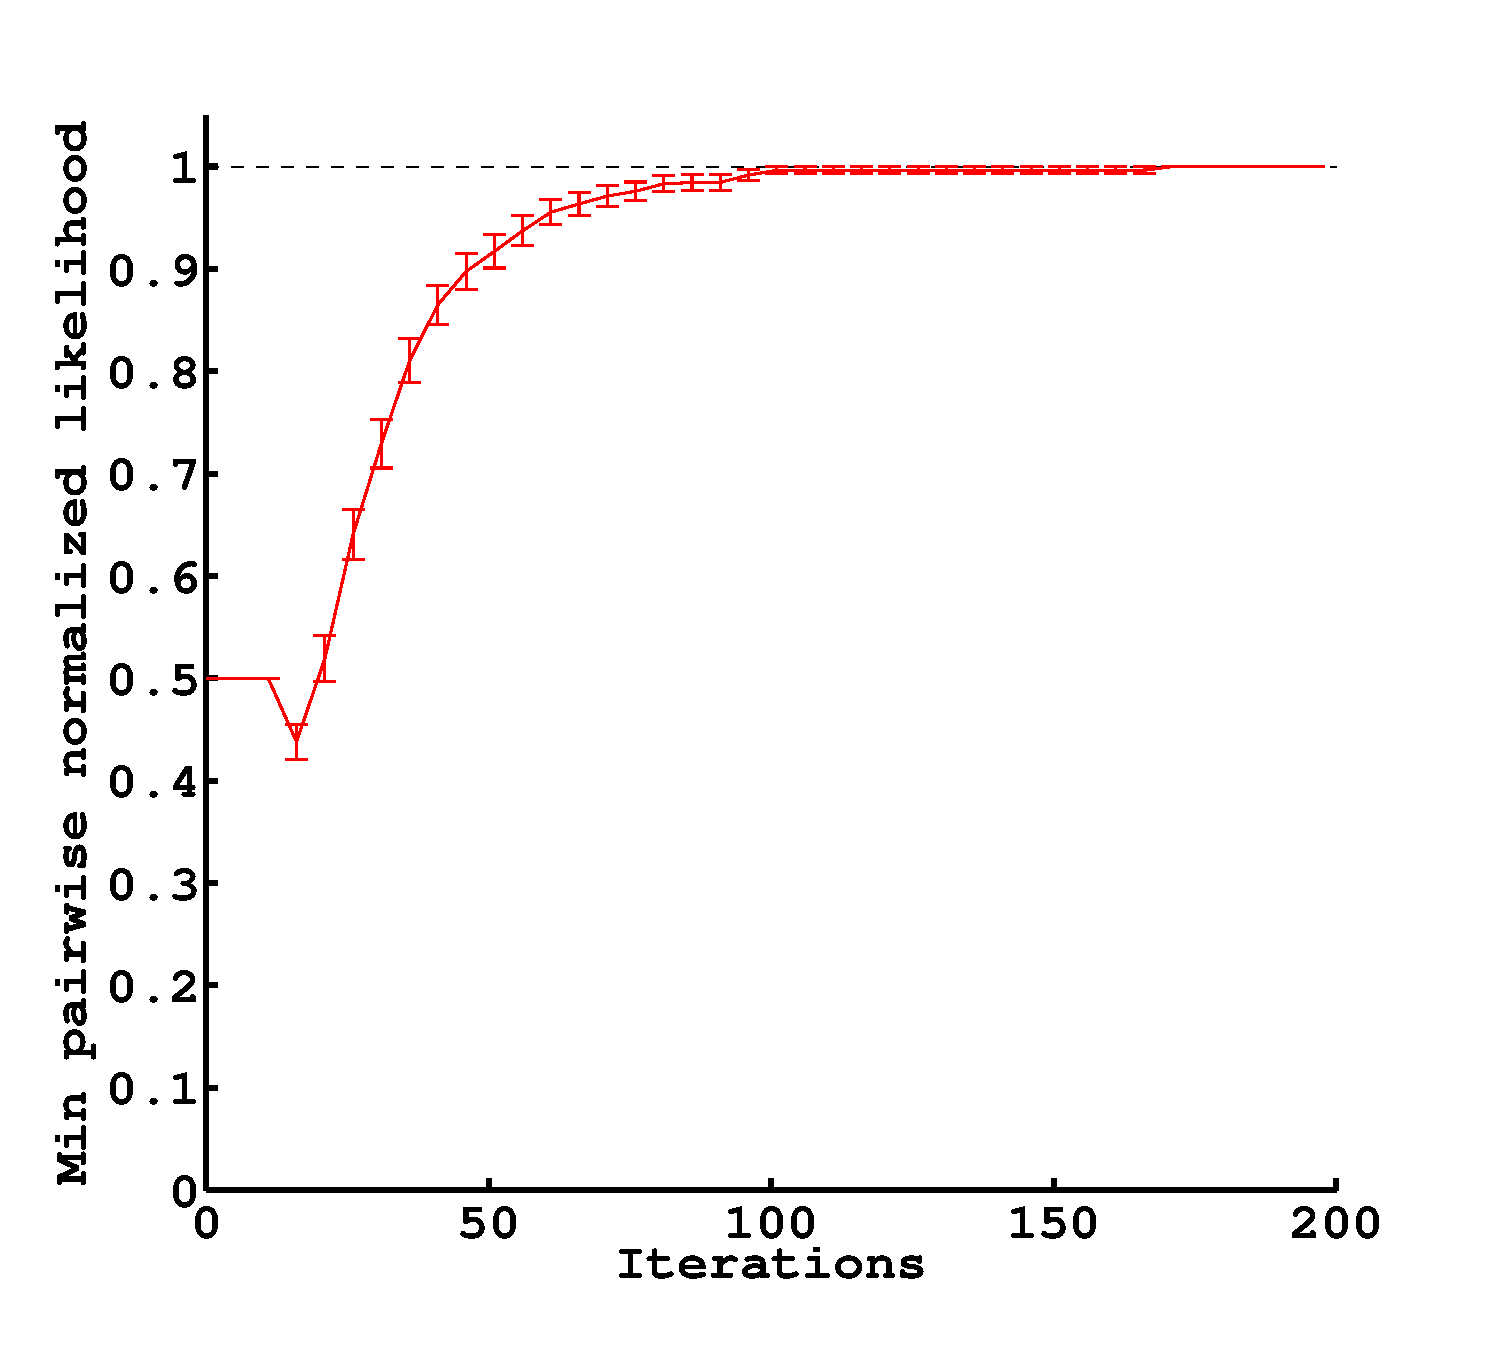
\includegraphics[width=\plotsize\columnwidth]{\imgpath/multiple_frame/multiple_frame_all_teacher.eps}
\caption{Evolution of the minimum of pairwise normalized likelihood for the correct hypothesis. After 200 steps, all our experiments identified with probability 1 the correct combination of task and interaction frame. Most of the experiments would have identified the task slighlty more than 50 steps with a confidence threshold of 0.9.}
\label{fig:multipleframeall}
\end{figure} 

We analyses in Figure~\ref{fig:multipleframefeedbackvsguidance} independently the case where the teacher was using the feedback (left) and guidance frame (right). We note that the behavior are the same for bot condition. only the guidance case took a bit longer for all hypothesis to converge to the correct task.

\begin{figure}[!ht]
\centering
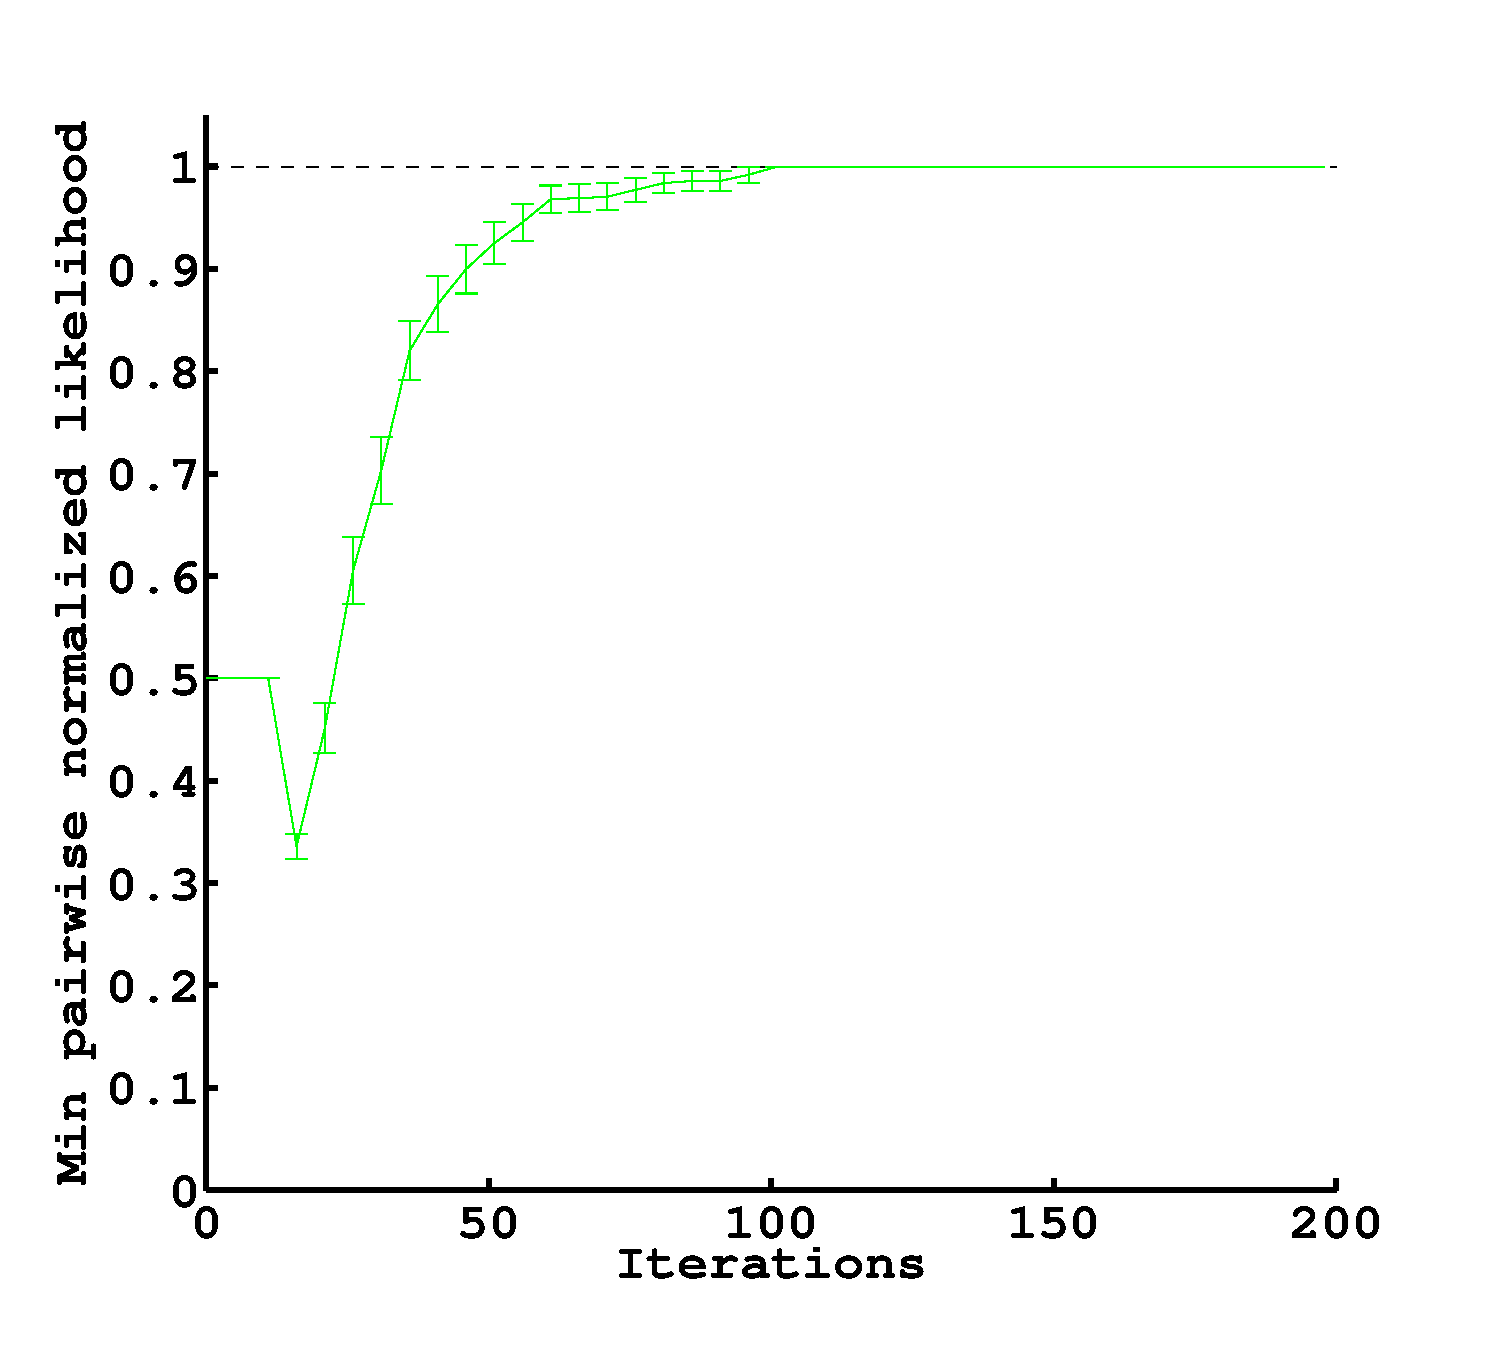
\includegraphics[width=0.49\columnwidth]{\imgpath/multiple_frame/multiple_frame_feedback_teacher.eps}
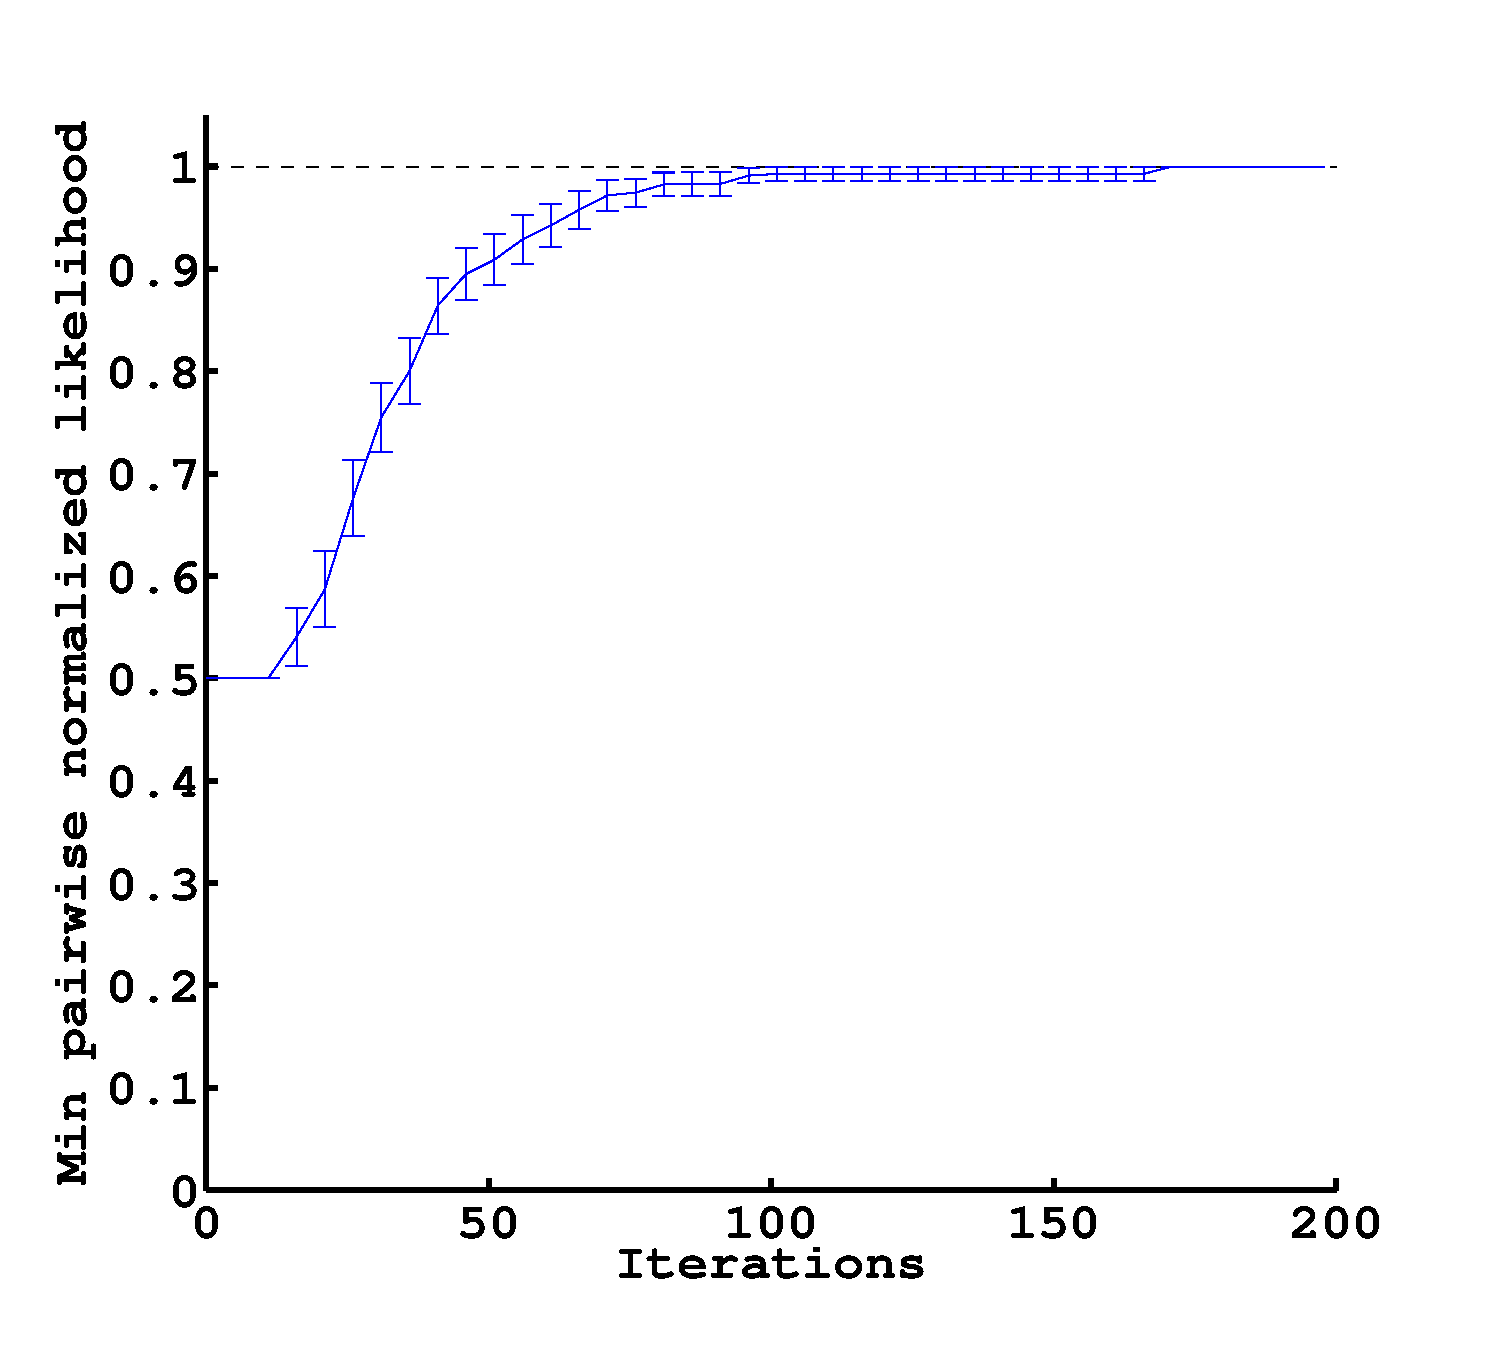
\includegraphics[width=0.49\columnwidth]{\imgpath/multiple_frame/multiple_frame_guidance_teacher.eps}
\caption{Evolution of the minimum of pairwise normalized likelihood for the correct hypothesis if the teacher provided feedback (left) or guidance (right) instruction. After 200 steps, all our experiments identified with probability 1 the correct combination of task and interaction frame. Most of the experiments would have identified the task in slighlty more than 50 steps with a confidence threshold of 0.9.}
\label{fig:multipleframefeedbackvsguidance}
\end{figure} 


\subsection{Discussion}

From those results in a simplistic environment, we can envision that following our interpretation hypothesis method for both task and interaction frame combination, one could start learning a task from unlabeled instructions and undefined interaction frames. In the end, our system would not only learn the task and the signal to meaning mapping, but also the interaction protocol used by the teacher.

Considering our example in section~\ref{chapter:limitation:continuoushypothesis}, an other potential use of the frame hypothesis scheme describe above would be to consider two different referential for the cardinal signal direction. Considering for example two cases, either the guidance signals are relative to the true North magnetic pole, either they are related to the current position of the user relative to the agent, or even relative to the current orientation of the robot (where going North would mean go straight). This experiment performed with a real robot, real users, considering a tablet, and different interaction frames has great potential to demonstrate the potential application of our work to a broader audience.

Finally a particle filter based method as used in section~\ref{chapter:limitations:continoushypothesis} for dealing with continuous task could be considered for dealing with a continuous set of interaction frame. For example, in our example of section~\ref{chapter:limitations:continousstate}, we used a parameterized frame that combines feedback and guidance frame (see Equation~\ref{eq:mixedfeedbackguidance}). By generating, testing, and resampling a set of those interaction frames we may be able to learn, not only the task and the signal to meaning mapping, but also the details of the interaction protocol used by the teacher. For example, in the experiment of section~\ref{chapter:limitations:continousstate} we may identify automatically the $\beta$ parameter of Equation~\ref{eq:mixedfeedbackguidance}.
% %!TEX root = ../../thesis.tex

\section{Human in the loop}
\label{chapter:limitations:userstudies}

\question{Do people want to have an open-ended choice about what signal to use? \\ Would they be more efficient?}

Only prerecorded datasets have been used. However, signals may change during the learning. For instance, people can try to adapt themselves to a robot if they believe the latter is not understanding properly. Or, brain signals are sensitive to the protocol, the duration of the experiment or even the percentage of errors made by the agent \cite{chavarriaga2010learning}. To which extend the behavior of our agent changes the properties of the teaching signal? 

Moreover, in real-world applications, users are usually told how to interact with machines. And having a free choice on some details of the interaction may finally become a disadvantage and lower perfomances. Do people want to have an open-ended choice about what signal to use? Would they be more efficient? When is it better to use a calibration procedure?

As we argued in the introduction, the work we presented is a starting point towards forms of adaptive interaction with non-technical users, that we may call fluid interaction learning. While we studied in this thesis properties of learning algorithms that will be needed for such an endeavor, it remains to be shown how they can be integrated within a full real-world human-robot interaction scenario and architecture so that the usability and acceptability of such system can be evaluated. Thus, user studies in particular will be a crucial next step of this work. The improvements described in previous section may be needed to reach acceptable levels of usability.

An interesting direction would be to consider the same experimental setup as the one used in chapter~\ref{chapter:humanexperiment} which allow to seamlessly use a human or a machine on either of the side of the interaction. A natural extension is therefore to replace the human builder by an agent using our algorithm. But one could also study active teaching algorithm \cite{cakmak2012algorithmic}, by replacing the teacher side by an artificial agent.

This kind of experiment would allow to study the same setup with both humans and artificial agents and may open new perspective in both human-robot interaction and experimental semiotic studies. By controlling some aspects of the interaction, on either of the interaction side, one could for example study how the agent behavior affect the teaching behavior of the human. But also study how the teaching behavior of a human influence the understanding and performance of the learner, whether the learner is a human or a machine. 

% algorithm assumption on human behavior

% discuss how the setup can be used in HRI, but also semiotic stuff...

% Users comply with the frame implemented. Same meaning, optimal strategies, timing...
% Assumption: The properties of the signals do not change wrt. the behavior of the agent

% In relation to targeting fluid interaction learning, we will consider in the future how more complex kinds of instructions can be included in our formalism. Indeed, the possible teaching models used spontaneously by people can be more complex than the simple meaning correspondences we assumed \cite{thomaz2008teachable,Cakmak2010optimality}. Also the turn taking scheme could be made more natural, as the robot could ask questions \cite{cakmak2012designing} and accept asynchronous instructions.

% Indeed, our current system can be restrictive for the user as the number of interaction increases quickly with the complexity of the size of the task and meaning spaces. However, we have shown that the system is able to use known sources of information, which in real-world interaction could be leveraged to keep the sample complexity low.
















%!TEX root = ../../thesis.tex

\section{Proof and formalism}
\label{chapter:limitations:proof}

It is of paramount importance to understand the properties of our algorithm, and to be able to have some certitude about its convergence and accuracy properties. The work presented in this thesis neglected this aspect and relied only on empirical evaluation. The next step for a motivated person it to work on a formalism of our problem and to derive some useful proof about some properties of the algorithm. In the following of this section we present a minimalist proof of the principle of our algorithm under extremely narrow condition.

\subsection{Problem and assumptions}

We consider a robot in a discrete state and action world. A teacher is providing feedback instruction to the robot through the use a simple interface with two buttons, one button for ``correct'' and one button for ``incorrect''. But the mapping between the buttons and the meanings is unknown to the robot at start.

This simplified setting, where the signals provided by the user, is certainly the first scenario that should have been considered in this work. Indeed it allows to study specific details of the algorithm in more details, without the influence of the classifier properties and  assumptions.

As for all our scenario, we assume that the user is coherent and uses one button for one meaning, and always the same button for the same meaning. Therefore, as exemplified in Figure~\ref{fig:proofmapping} the mapping between symbolic signals and their meaning can only be of two forms. 

\begin{figure}[!ht]
\centering
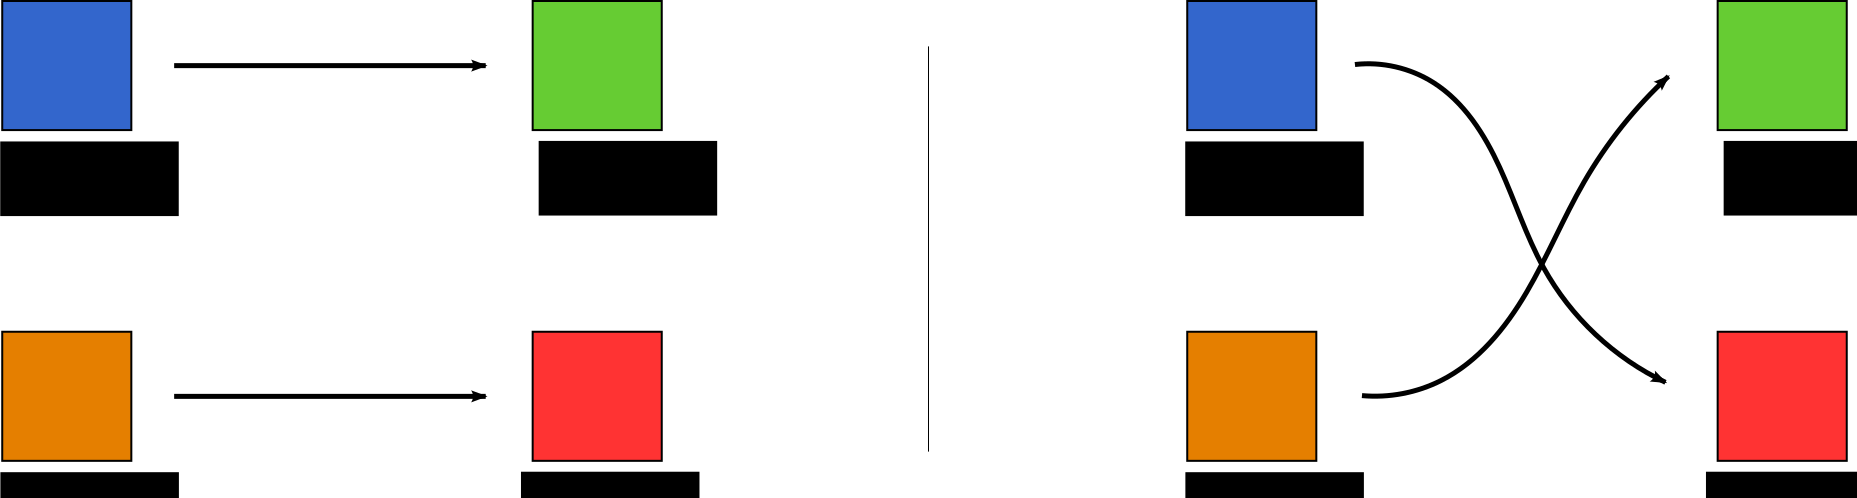
\includegraphics[width=\columnwidth]{\visualspdf/proof/mappings.pdf}
\caption{The two possibles button to meaning mapping.}
\label{fig:proofmapping}
\end{figure} 

We further assume the robot is provided with a set of task hypothesis ($\xi_1,\ldots,\xi_T$), represented by their associated policies ($\pi_1, \ldots, \pi_T$). This set includes the task $\hat{\xi}$, the teacher as in mind, and when the robot performs a non-optimal action according to the optimal policy $\hat{\pi}$ associated to this task, the teacher presses the button associated to the ``incorrect'' meaning. Respectively pressing the  the button associated to the ``correct'' meaning for an optimal action. Finally we assumed that the teacher never makes teaching mistakes.

We define a number of terms that will simplify the notation in further subsections. $nS$ is the number of states in the environment, $nA$ is the number of actions available to the robot, and $nSA$ is the number of state-action pairs an agent can visit, which is simply $nS * nA$. We note as $diff(\pi_t, \pi_u)$ the number of optimal state-action pairs that differs between the optimal policies $\pi_t$ and $\pi_u$ respectively associated to the task $\xi_t$ and $\xi_u$. Therefore the ratio of optimal state-action pairs that differs between two task hypothesis is denoted as $\frac{diff(\pi_t, \pi_u)}{nSA}$. 

The $diff()$ function logically outputs $0$ when comparing one task to itself, i.e. $diff(\pi_t, \pi_t) = 0$. A ratio of 0 between two tasks means they are the same. And, as discussed in chapter~\ref{chapter:lfui:symmetries}, a ratio of 1 means the two tasks are symmetric which means whatever the action the robot will choose, the meaning inferred according to the first task will be the opposite of the meaning inferred according to the second task. This property, as will be seen in our minimalist proof, do not allow to differentiate between two symmetric task.


\subsection{Illustration}

Before describing our simple proof, it is important to have an intuition on the relation between the buttons and the meanings in different condition. We will consider again our T world scenario as an illustration (see chapter~\ref{chapter:lfui:example}).


Figure~\ref{fig:proofsymbolic} shows all possible button presses sequence expected from the teacher in different condition. On top are the state-action pair considered (a). (b) and (c) lines represent the expected meanings for each of the state-action pairs and according to the hypothesis G1 (b) or G2 (c). (d) and (e) lines represent the possible button presses sequence of the teacher when teaching hypothesis G1 and considering the two possible mappings. Respectively (f) and (g) for hypothesis G2.

\begin{figure}[!ht]
\centering
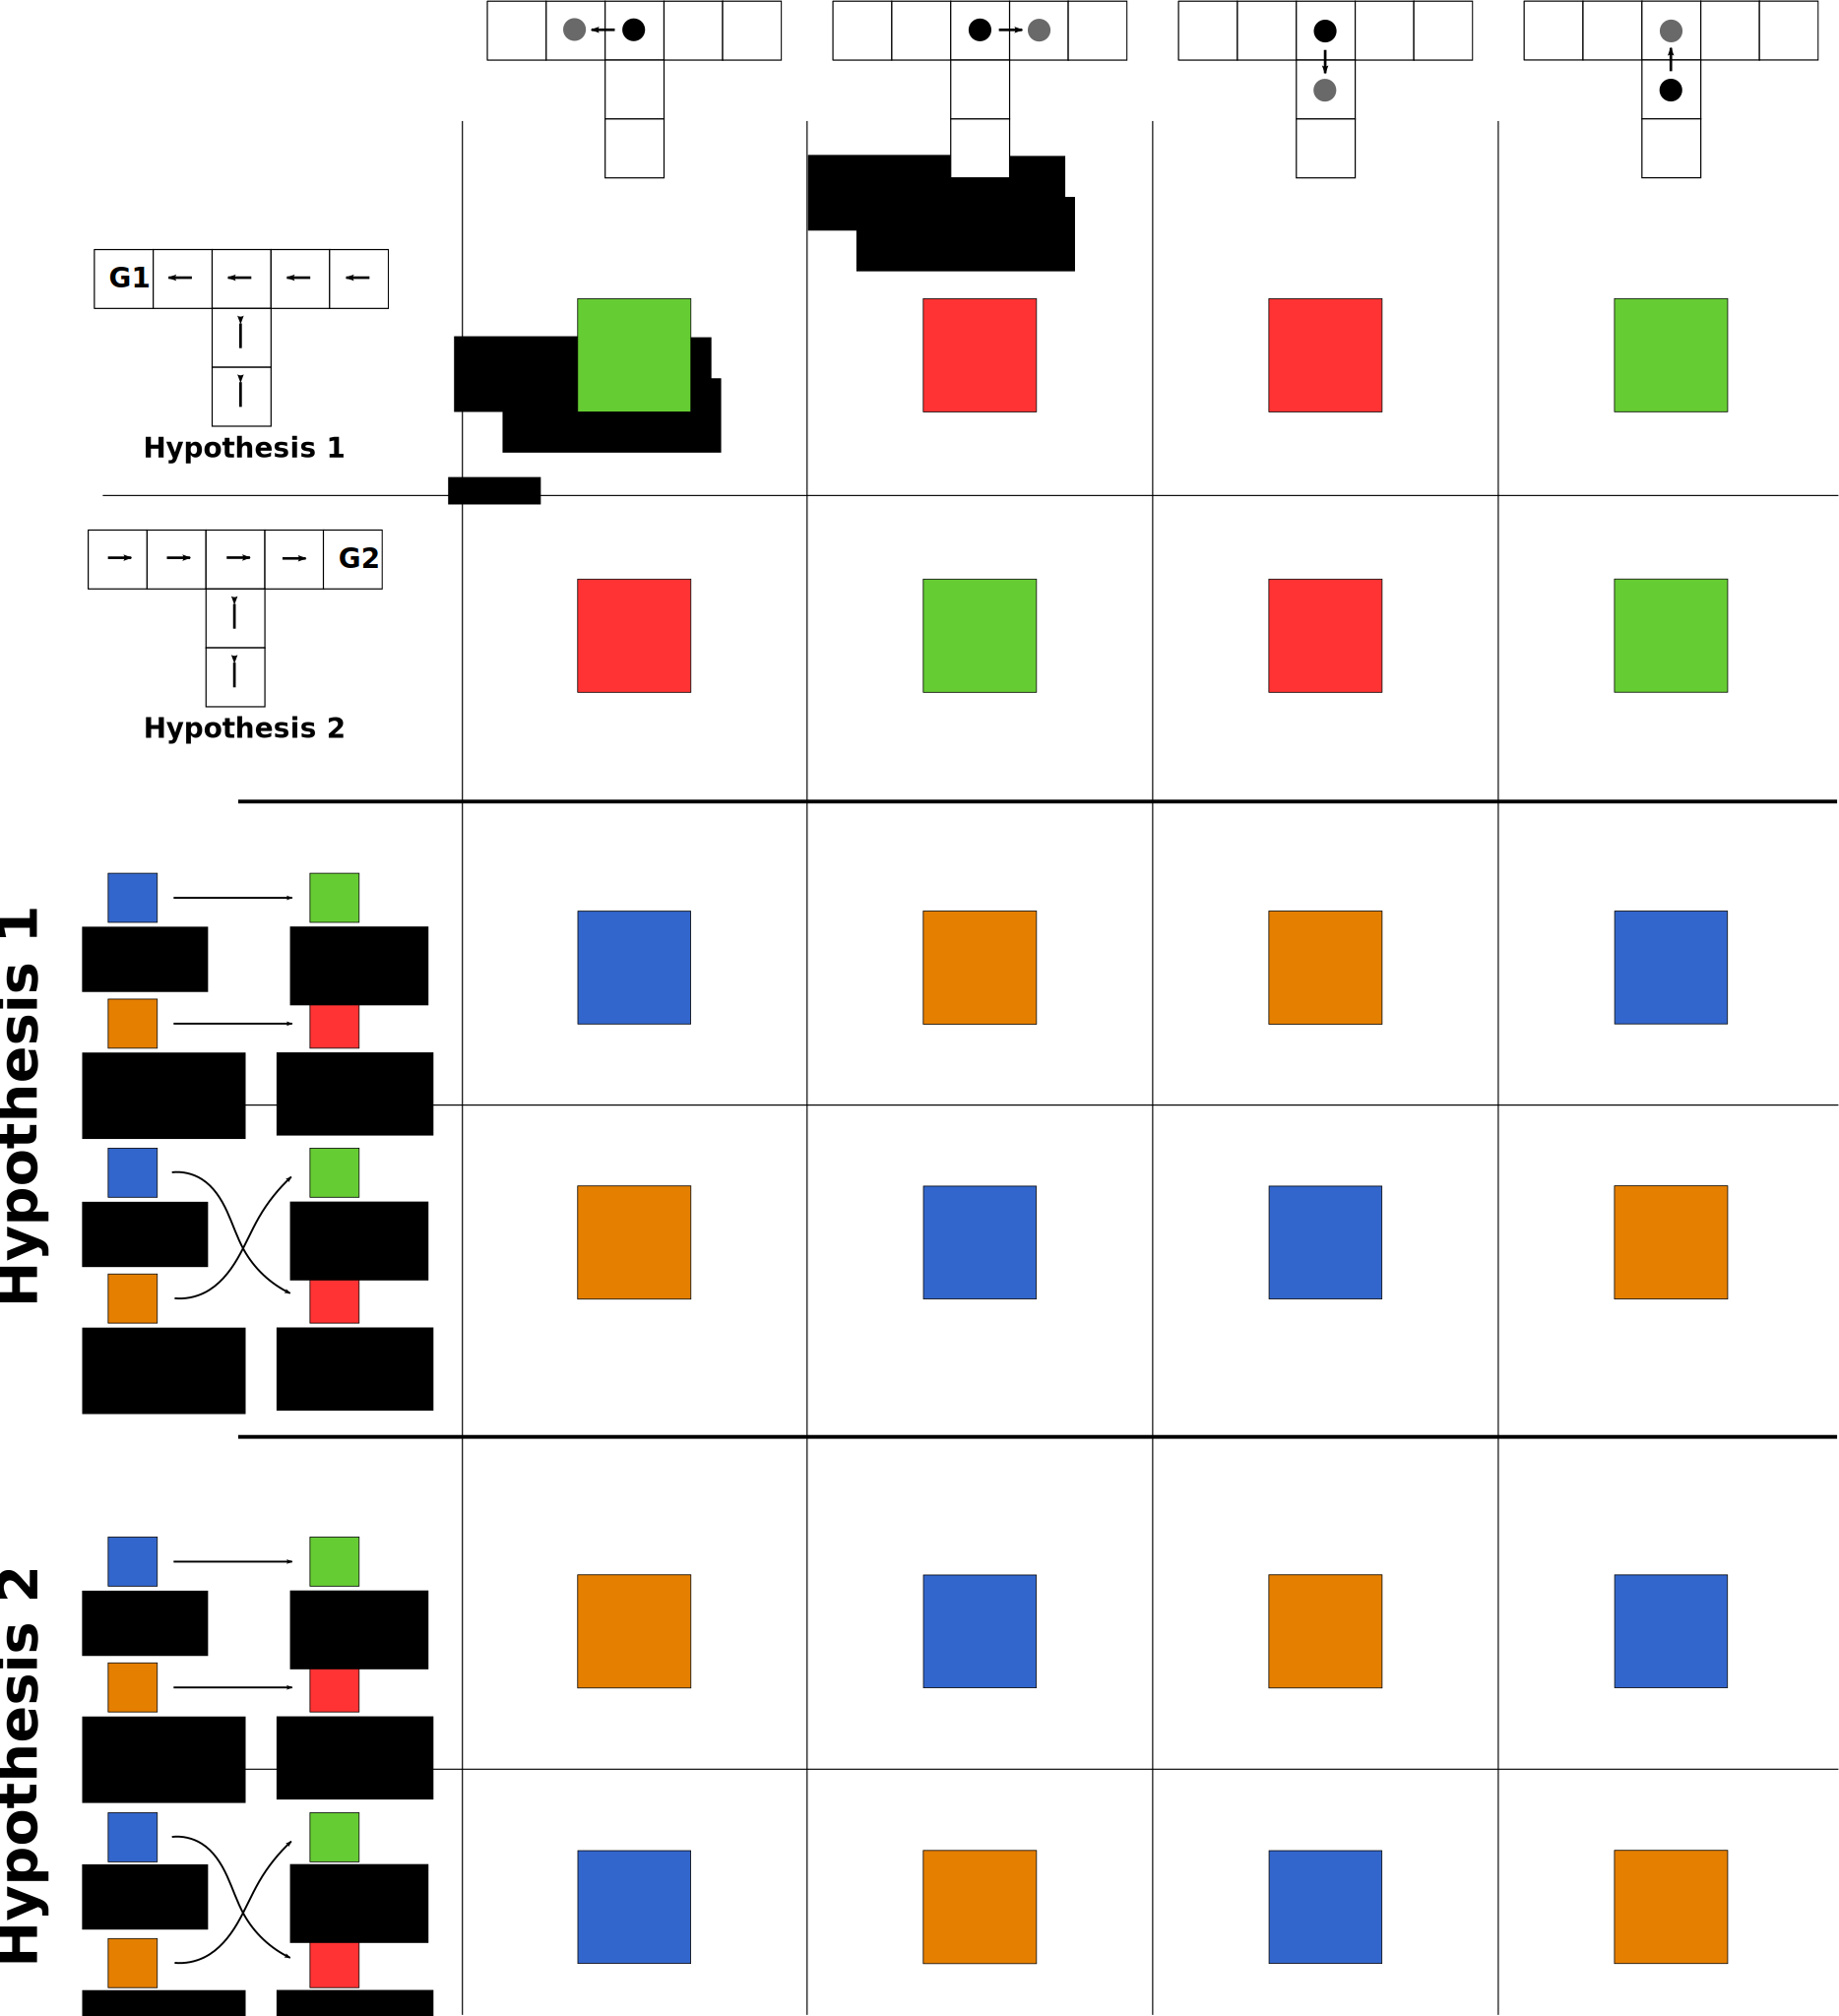
\includegraphics[width=\columnwidth]{\visualspdf/proof/symbolic_feedback.pdf}
\caption{Illustration of the teacher's button presses for several state-action pairs. On top are the state-action pair considered (a). (b) and (c) lines represent the expected meanings for each of the state-action pairs and according to the hypothesis G1 (b) or G2 (c). (d) and (e) lines represent the possible button presses sequence of the teacher when teaching hypothesis G1 and considering the two possible mappings. Respectively (f) and (g) for hypothesis G2.}
\label{fig:proofsymbolic}
\end{figure} 

First, before entering into more details, given the extensive number of assumptions defined, for the simple example of Figure~\ref{fig:proofsymbolic} it would be easy to find the correct hypothesis by visiting only two state-action pairs. Indeed as taking an action in the trunk of the T will produce similar responses from the teacher for all hypothesis, and that the user if not making teaching mistakes and is coherent in its use of the buttons, we would instantaneously know the meaning of the button pressed and therefore the meaning of the other button. Then taking an action in the top bar of the T would allow us to differentiate between G1 and G2. However we will not exploit this type of properties for our proof and we remind that in all the experimental scenarios presented in this thesis, there were no state-action pairs that allowed for an unequivocal interpretation of a signal.

Now, for the purpose of our demonstration, we should read this figure by comparing lines (d), (e), (f), and (g) with the expectation from lines (b) and (c). We will denote $B$ the blue button, O the orange button, $C$ the ``correct'' meaning (the green patch), and $W$ the ``incorrect'' meaning (the red patch, $W$ for wrong). For example, let's imagine we receive the sequence of presses of line (d) which we note $[B,O,O,B]$. For hypothesis 1 (G1) we expected $[C,W,W,C]$, and for hypothesis 2 (G2) we expected $[W,C,W,C]$. 

Given this two possible interpretation we can build a statistical model for the signal to meaning mapping. For G1, we obtain the following model $p(C|B, G1) = \frac{2}{2} = 1$, $p(C|O, G1) = \frac{0}{2} = 0$, and $p(W|B, G1) = \frac{0}{2} = 0$, $p(W|O, G1) = \frac{2}{2} = 1$. To simplify notation we note $[1,0]_{B,G1}$ and $[1,0]_{O,G1}$ the model for each button where the first element of the vector is the probability associated to the ``correct'' meaning and the second is the one associated to the ``incorrect'' meaning. And the underscript details the button and the task considered. Using the same reasoning, again for line (d) but for hypothesis G2, the classifier is: $[0.5,0.5]_{B,G2}$ and $[0.5,0.5]_{O,G2}$.

In this thesis, as we were not considering symbolic signals, we used a metric that compares the expectation from the frame (i.e. lines (b) and (c)) with a classifier associated to each task. Let's use Equation~\ref{eq:matchingoverfitting} to compute the likelihood for each task. For G1 we obtain:
%
\begin{eqnarray}
\L(G1) &=& \left((1\times1)+(0\times0)\right)\left((0\times0)+(1\times1)\right)\left((0\times0)+(1\times1)\right)~\ldots  \nonumber \\
&& \ldots~\left((1\times1)+(0\times0)\right)  \nonumber \\
&=& 1 \nonumber
\end{eqnarray}

And for G2 we obtain:
%
\begin{eqnarray}
\L(G2) &=& \left((0.5\times0)+(0.5\times1)\right)\left((0.5\times1)+(0.5\times0)\right)~\ldots  \nonumber \\
&& \ldots~\left((0.5\times0)+(0.5\times1)\right)\left((0.5\times1)+(0.5\times0)\right) \nonumber \\
&=& 0.0625 \nonumber
\end{eqnarray}

By normalizing the likelihoods, we obtain the probability of each task: $p(G1) \approx 0.94$ and $p(G2) \approx 0.06$. We see that our measure of likelihood is able to identify the correct task. The same process can be repeated for each cases (i.e. (e), (f), and (g)) and will always identify the correct hypothesis. 

Given this explanation, we are ready to move on for the actual proof, in which to simplify the proof, we will add an additional assumption.

\subsection{The proof}

In order to make the proof simple, we assume each hypothetic policy has an equal number of optimal state-action pairs than of non-optimal state-action pairs. Therefore when the agent has visited once all the state-action pairs, it has collected, for each hypothesis, the same amount of signals with label ``correct'' than with label ``incorrect''. As a consequence, this properties ensures that the signal to meaning model for each class (i.e. for $C$ and $W$) are symmetric. 

We can explain this effect as follows. First, for all hypothesis this assumption ensure that, when the agent has visited once all the state-action pairs, the user will have pressed as many time the blue button than the orange button, exactly $\frac{nSA}{2}$ times. And the same assumption ensures that whatever the task considered the number of ``correct'' and ``incorrect'' labels will be the same. However the number of blue button presses associated to ``correct'' or ``incorrect'' labels remains undefined and depends on the overlap between the true unknown policy taught by the teacher and the one considered by the agent in the labeling process. 

Therefore, we can evaluate the possible mapping models based on the difference in policies between the optimal task and any hypothetic task using our $diff()$ function defined earlier. For a given task $\xi_t$ we can compute the ratio of optimal state-action pairs that are the same as for the true task $\hat{\xi}$, which we denote $\Upsilon_{\xi_t} = \frac{nSA - diff(\pi_t, \hat{\pi})}{nSA}$. Obviously the agent will never have access to this information and we only use this measure for our proof.

Given our previously defined assumption, and assuming the agent visited all state-action pairs once, if the user uses the blue button to mean ``correct'', then the blue signal model will be $[\Upsilon_{\xi_t},1-\Upsilon_{\xi_t}]_{B,\xi_t}$. Which implies the orange button mapping is $[1-\Upsilon_{\xi_t},\Upsilon_{\xi_t}]_{O,\xi_t}$. Respectively, if the user uses the blue button to mean ``incorrect'', then the blue signal model will be $[1-\Upsilon_{\xi_t},\Upsilon_{\xi_t}]_{B,\xi_t}$. Which implies the orange button mapping is $[\Upsilon_{\xi_t},1-\Upsilon_{\xi_t}]_{O,\xi_t}$. 

As there is the same number of ``correct'' and ``incorrect'' expected labels, we can factorize the likelihood equation as follow (see appendix~\ref{appendix:proof}):
%
\begin{eqnarray}
\L(\xi_t) &=& \Upsilon_{\xi_t}^{nSA.\Upsilon_{\xi_t}} \times (1-\Upsilon_{\xi_t})^{nSA.(1-\Upsilon_{\xi_t})}
\label{eq:likelihoodproof}
\end{eqnarray}

Note that this equation is the same whatever the button chosen by the user to mean ``correct''. We can check our previous likelihood estimate in our simple example of Figure~\ref{fig:proofsymbolic} considering the 4 state-action space visited are the only one available in the world, and considering we receive button presses as in line (d). We obtain the same likelihoods as the one derived in the first subsection, i.e. $\L(G1) = 1^{1\times4} \times 0^{0\times4} = 1$ and $\L(G1) = 0.5^{0.5\times4} \times 0.5^{0.5\times4} = 0.5^4 = 0.0625$.

Let's plot the likelihood function with respect to the full range of value that $\Upsilon_{\xi_t}$ can take, i.e. between 0 and 1. We consider that $nSA = 1$ for now. Obviously such a value of $nSA$ is impossible in practice given our assumptions, we need as many optimal and non-optimal state-action pair, which means that $nSA$ must be an even number. However, now that we have our theoretical estimate of the likelihood function we shall study its properties in a theoretical way. Additionally, our equation is only valid if the agent visited all state-action pair but for the sake of our analysis, we consider that the value of $nSA$ represents the number of state-action pair visited by the agent. Moreover, there exist a relation between the number of state-action pair and the discrete set of value that $\Upsilon_{\xi_t}$ can take given our assumptions, but for the sake of the analysis we consider the full range of value between 0 and 1.

Figure~\ref{fig:prooflikelihoodone} shows the likelihood function for $nSA = 1$. As expected the likelihood value is higher for the correct task, i.e. when $\Upsilon_{\xi_t} = 1$, and decrease as the number of state-action pairs that differ increase, i.e. when $\Upsilon_{\xi_t}$ decrease. However this function holds an interesting property, which is that once more than half of the optimal state-action pair differs with the true task, the function increases again. Until is reaches a point where none of the optimal state-action pair of the task are the same as for the true task. This specific case is what we called symmetric task hypothesis, where the symmetric interpretation of the feedback signals is as likely as  the correct interpretation of the signals. Indeed none of the state-action pairs allow to break this symmetry for the feedback frame. 

Therefore, given all the assumptions considered, if the agent is provided with a set of task hypothesis, that included the correct task $\hat{\xi}$ but does not include any symmetric hypothesis --- which means all tasks hold the following property $\Upsilon_{\xi_t} > 0$ ---, we can guarantee that if the teacher visits all state-action pairs once, the user intended task $\hat{\xi}$ --- which hold the property $\Upsilon_{\xi_t} = 1$ --- will have the greater likelihood. In other words: $\L(\hat{\xi}) > \L(\xi_t)$ if $\Upsilon_{\xi_t} \in~]0,1[$.

\begin{figure}[!ht]
\centering
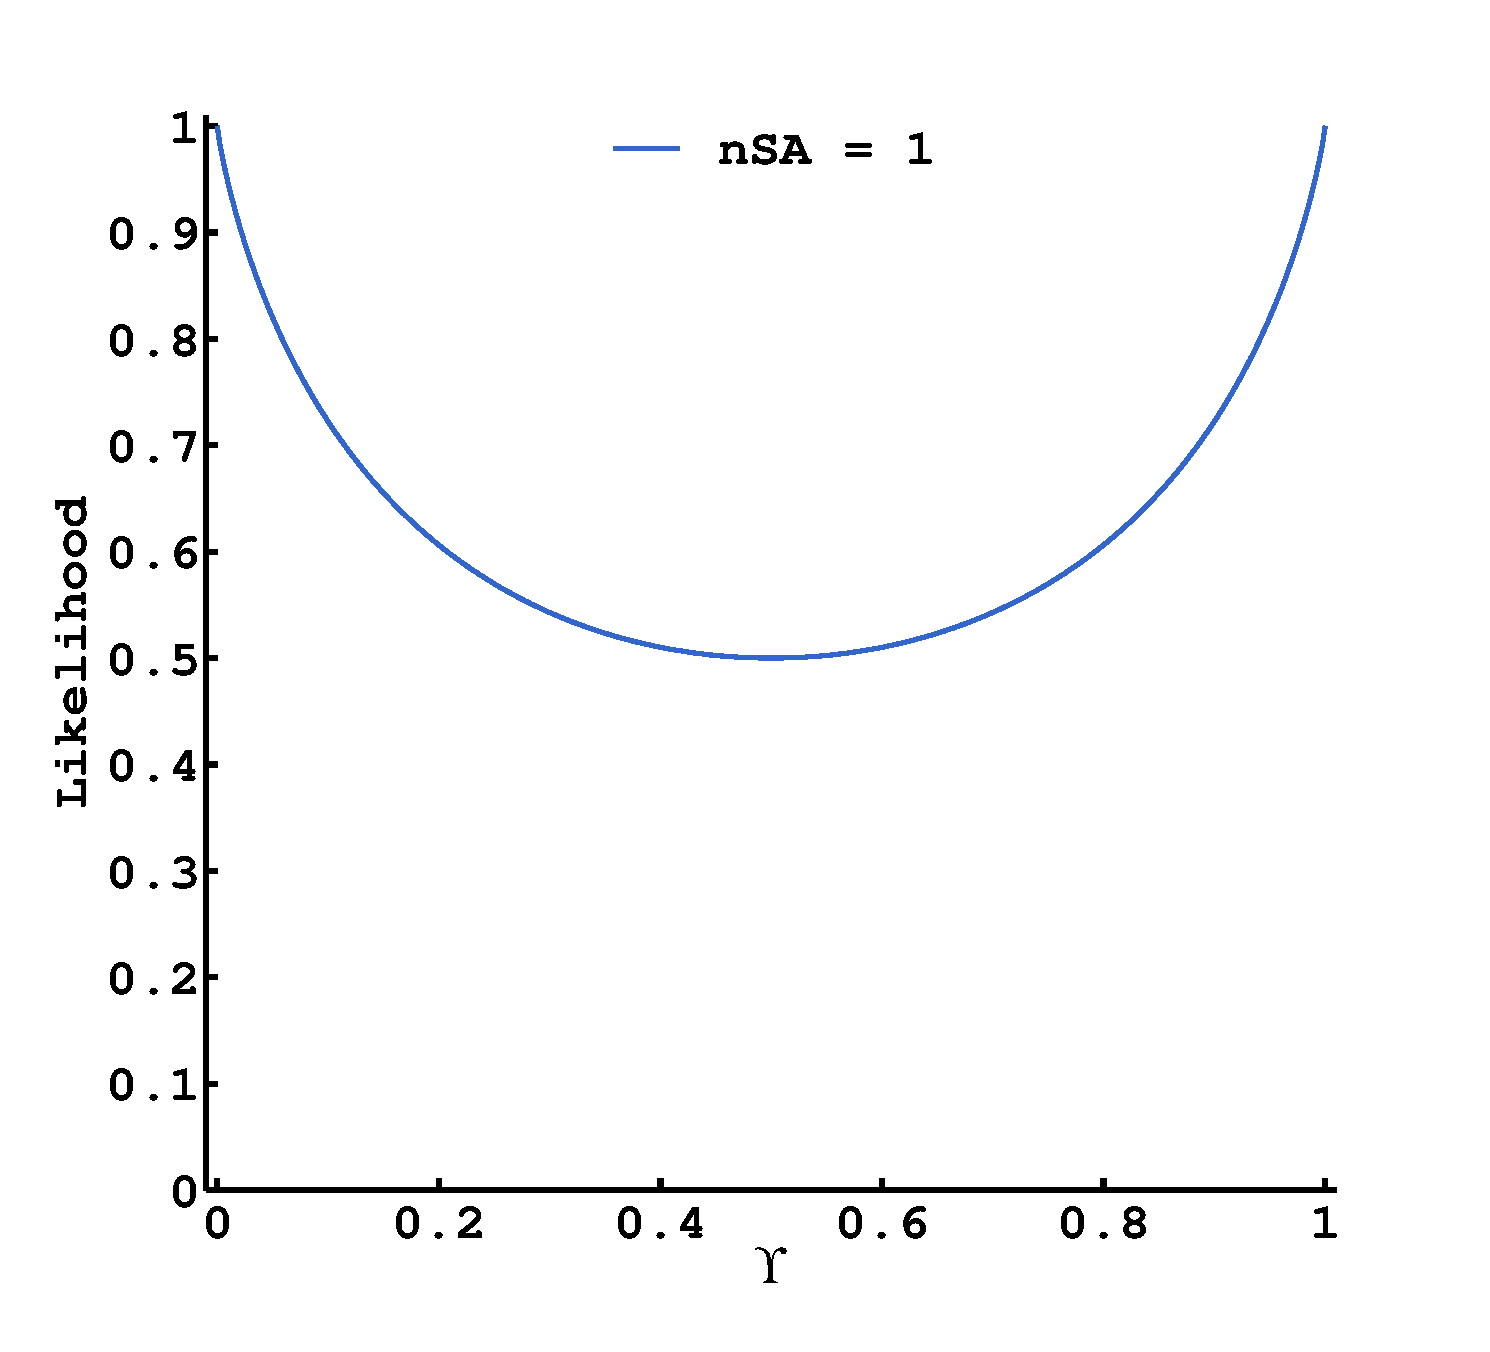
\includegraphics[width=\plotsize\columnwidth]{\imgpath/proof/likelihoodOne}
\caption{The likelihood function of Equation~\ref{eq:likelihoodproof} for $nSA =1$.}
\label{fig:prooflikelihoodone}
\end{figure}

We now discuss the problem of estimating our confidence that one task is a better candidate than an other one. Of course, in this setting, given the strong assumption that the user is never making mistakes, such confidence mechanism is not needed. However, we have seen in previous chapter that deciding when to stop is a critical part of the algorithm. The simplest method consist of normalizing the likelihood for each task defining a probability threshold above which a task is considered as the correct one. If we consider for example 10 task hypothesis with different values of $\Upsilon$, normalizing the likelihood when $nSA = 1$ won't produce a very sharp probability distribution on task. All task will roughly share the same probability. However, when visiting more and more states, the likelihood function becomes more and more sharp and only normalizing likelihoods will split the hypothesis apart. In the limit, when $nSA \rightarrow +Inf$, only the hypothesis with a better value of $\Upsilon$ (i.e. closer to 0 or 1) will reach a probability of 1.

\begin{figure}[!ht]
\centering
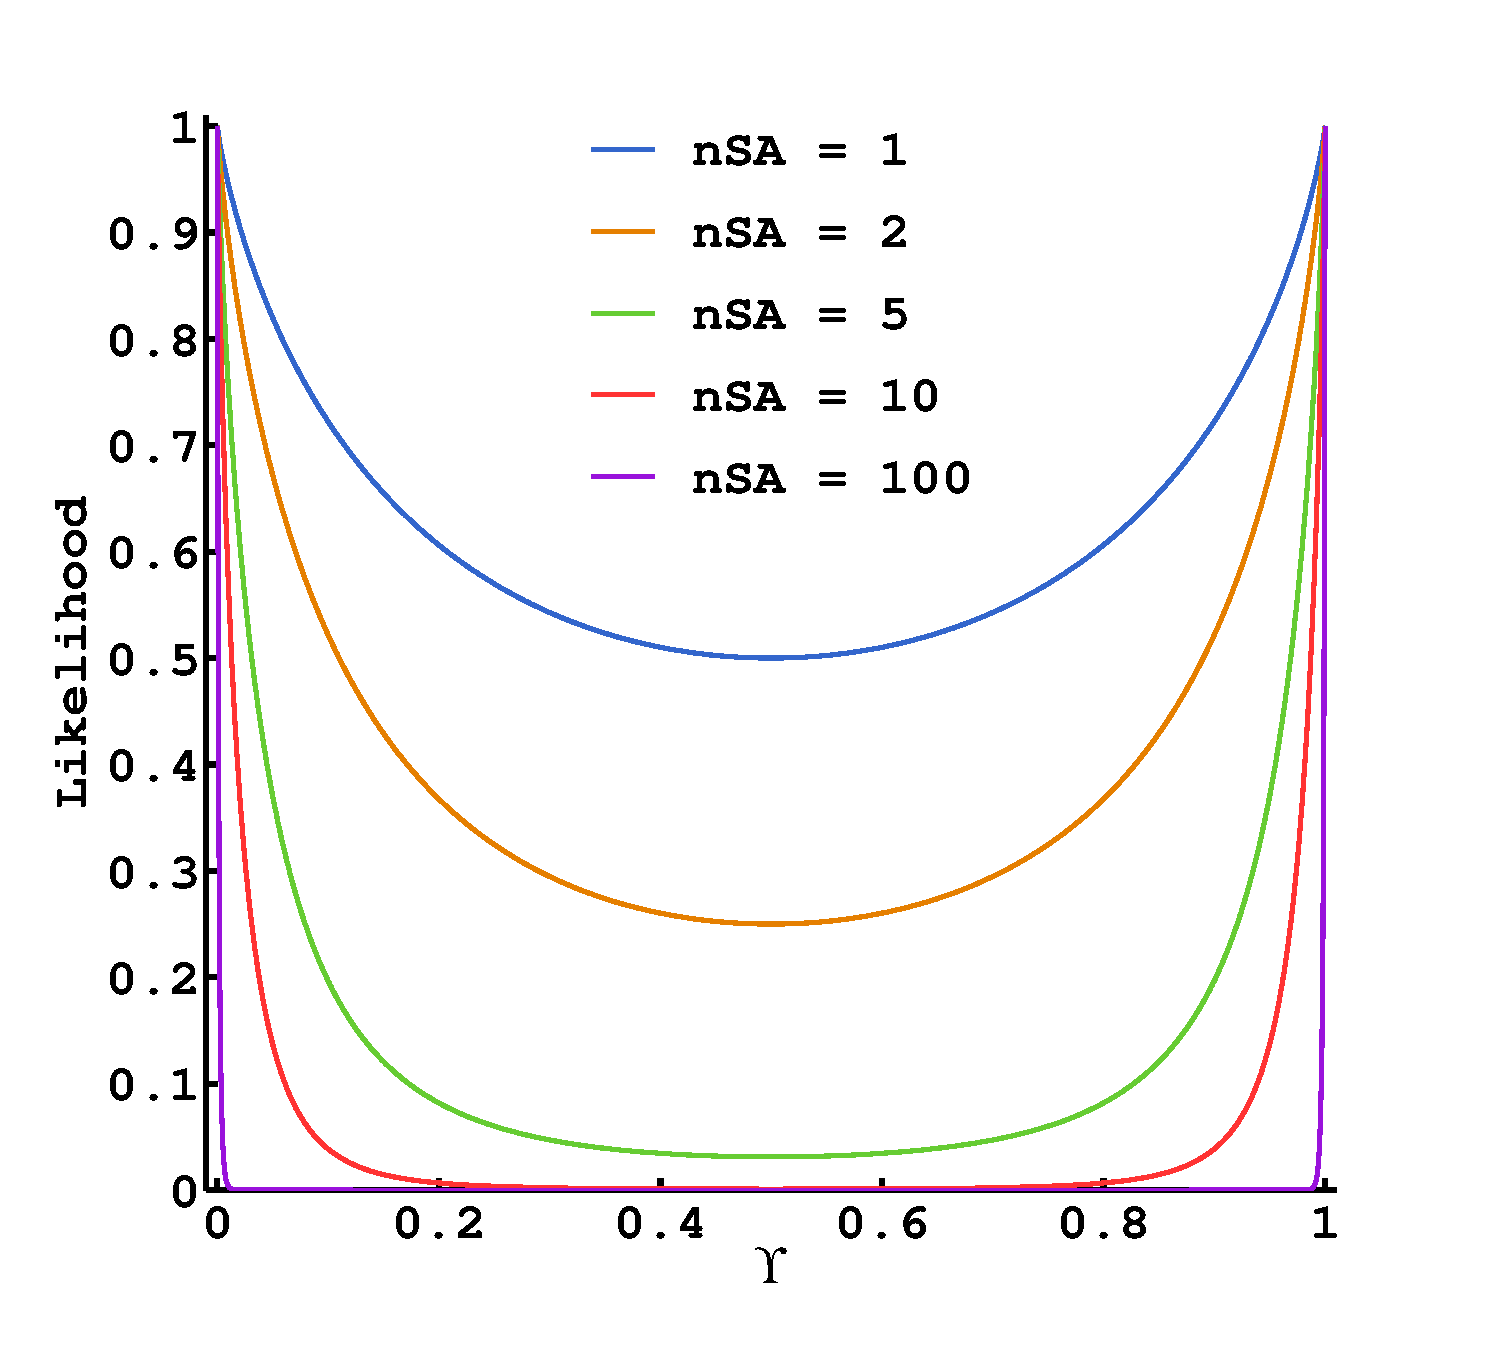
\includegraphics[width=\plotsize\columnwidth]{\imgpath/proof/likelihoodMany}
\caption{The likelihood function of Equation~\ref{eq:likelihoodproof} for $nSA =1,2,5,10,100$. The more we have collected evidence, the more the difference is sharp between task hypothesis.}
\label{fig:prooflikelihoodmany}
\end{figure}

This model allows to understand in more conceptual terms some properties of our algorithm. And in practice very few of the assumption considered are applicable in our experimental setups.

Finally, for illustration purpose, we present a world holding all our assumption properties, we named it the clock world (see Figure~\ref{fig:clockworld}). This world has 12 states, which we represent as the hours on a clock. The agent has two actions available: turning clockwise or counter-clockwise. The user wants the agent to reach one of 12 states. This world is the extension of the line word but where the line loops on itself.

\begin{figure}[!ht]
\centering
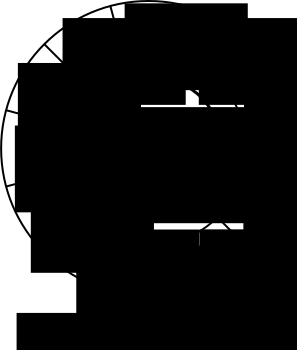
\includegraphics[width=0.3\columnwidth]{\visualspdf/proof/clockworld.pdf}
\caption{Illustration of the clock world. The agent has two actions available: turning clockwise or counter-clockwise. The user wants the agent to reach one of 12 states.}
\label{fig:clockworld}
\end{figure} 

\subsection{Why not using the entropy of the meaning models?}

We continue here the discussion about the difference between the method detailed in this thesis work and the method presented in section~\ref{chapter:limitations:overlap}. In section~\ref{chapter:limitations:overlap}, we tried to differentiate the task by looking at the overlap of the model for each class. In other words, we tried to evaluate the uncertainty of the signal model fitted for each task, and we selects the one that as lower uncertainty.

We can do the same in our simple example, indeed, as we assumed that the user is coherent in his button presses, the task whose associate button presses model is the less uncertain is the more likely to be the correct one. Given the history of interaction, we can model the button presses of the user as Bernoulli variables, which can take only two values ``correct'' or ``incorrect'', such as a coin flipping problem. Following the previous development, we can compute the probability that the user will press the blue button to mean ``correct'', which is $\Upsilon_{\xi_t}$ (or $1-\Upsilon_{\xi_t}$ if the orange button is used for ``correct'').

The binary entropy function, denoted $H_{\mathrm b}(p)$, is the entropy of a Bernoulli process with probability of success p, and can be computed as follows:

\begin{eqnarray}
H_{\mathrm b}(p) = -p\log_2(p) - (1-p)\log_2(1-p) 
\label{eq:likelihoodentropy}
\end{eqnarray}

The binary entropy function is shown in Figure~\ref{fig:prooflikelihoodentropy}. As one would expect the shape of the entropy function holds similar properties than our likelihood Equation~\ref{eq:likelihoodproof}.
    
\begin{figure}[!ht]
\centering
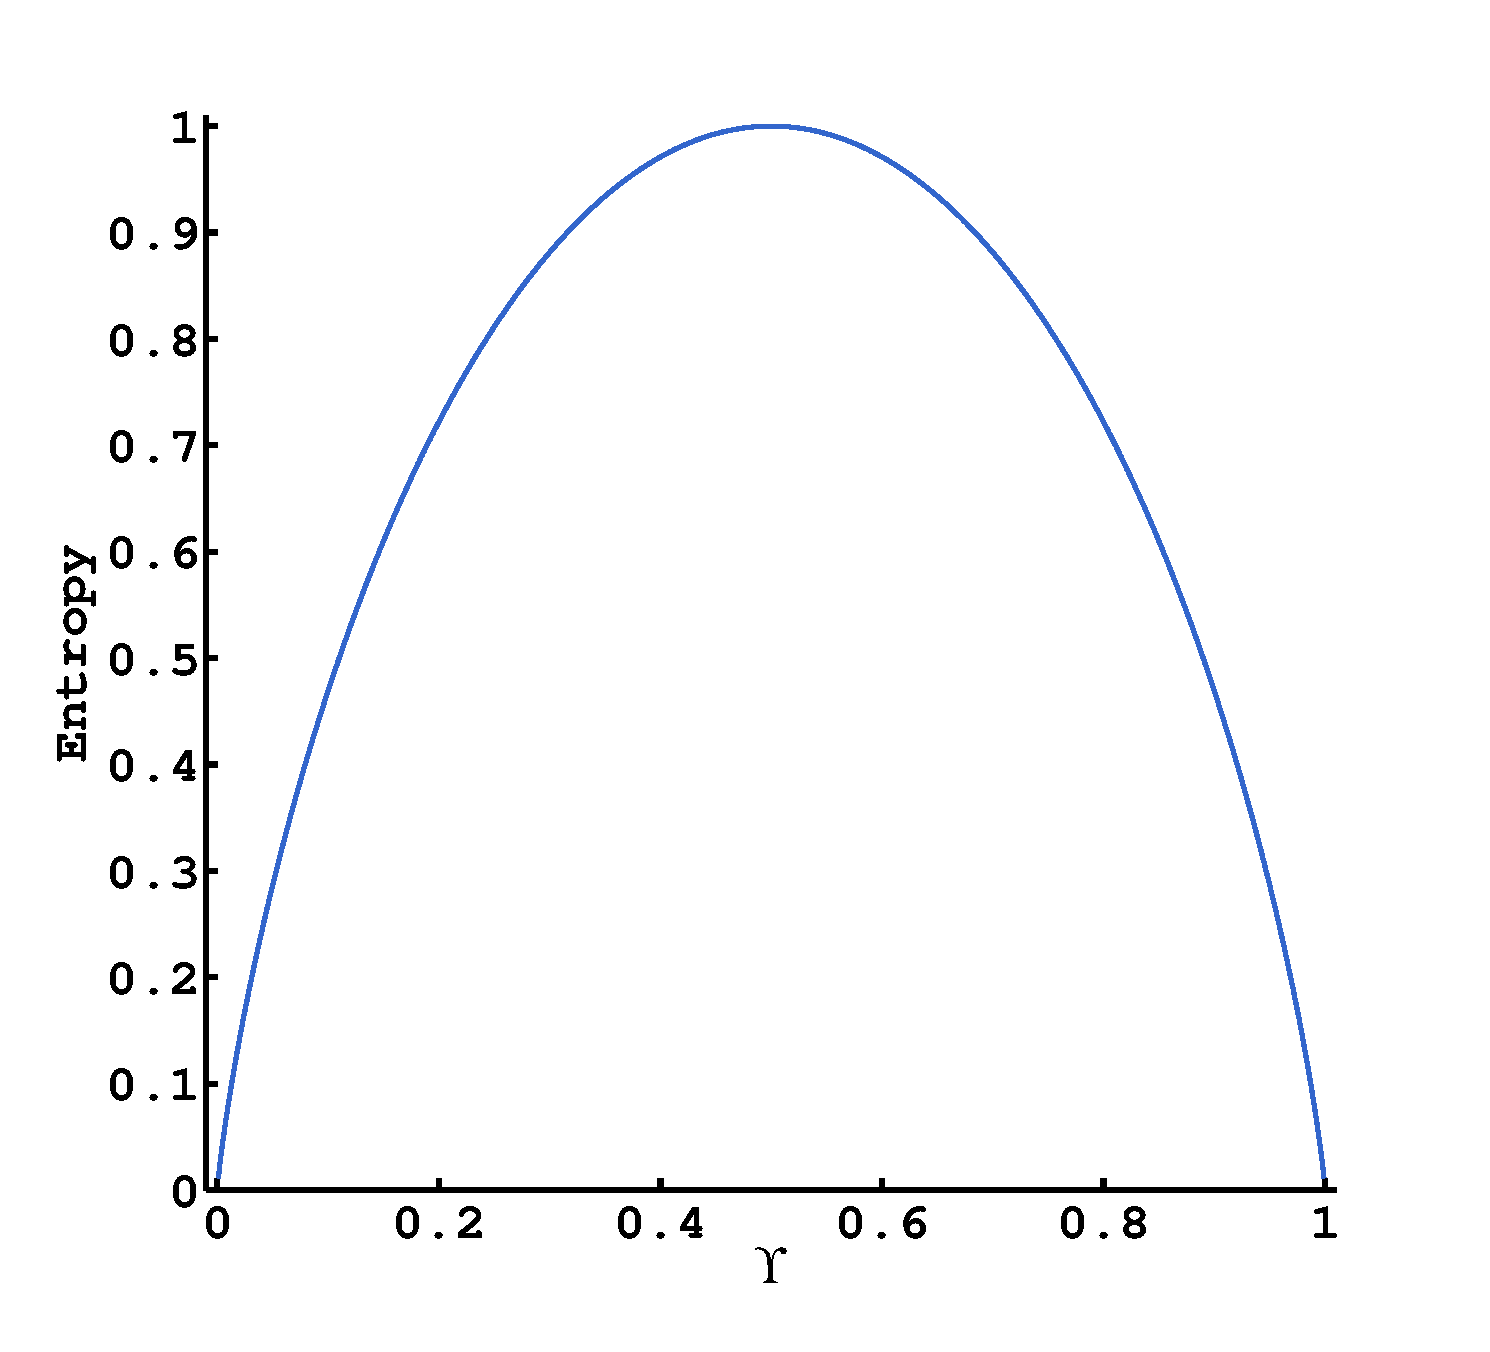
\includegraphics[width=\plotsize\columnwidth]{\imgpath/proof/entropy}
\caption{The binary entropy function.}
\label{fig:prooflikelihoodentropy}
\end{figure}

This method allow us to rank correctly our task hypothesis with respect to the uncertainty of their estimated models. However, this function will not ``sharpen'' as the likelihood Equation~\ref{eq:likelihoodproof} when the agent visit more and more states. The only change will result in a better approximation of the Bernoulli process modeling the button presses.

Therefore, this method alone is not enough to estimate which task is the correct one as one should also measure the uncertainty of the measure of uncertainty. To do so, we propose to use beta distribution, which is the conjugate prior probability distribution for the Bernoulli distributions. A beta distribution would describe the initial knowledge concerning probability of button presses and would be updated as new information comes in. Finally, by comparing between the beta distribution associated to each task, we could expect to find a suitable measure of task confidence. The interested readers may refer to \cite{montesano2012active} for a practical robotic example using this process.

\subsection{Discussion}

While it is always interesting and useful to formulate proof of algorithm, the restricted assumption used in this section makes it impossible to use this results in practical scenario. But we note that our experimental results shows that our algorithm can work with fairly good performance on different scenarios using continuous signals as noisy as EEG signals.

I personally have very few experience in making proof for such kind of problems and it may be useful to pursue in that direction by releasing some of the assumption steps after steps. Starting with the assumption that all hypothesis have half of their state-action pair optimal and half non-optimal, and progressively accounting for some teaching mistakes. Reaching that level of proof would already offer some guarantees for simple scenario using discrete state, discrete action, and symbolic signals but under more realistic teaching condition.


%%%%%%%%%%%%%%%%%%%%%%%%%%%%%%%%%%%%%%%%%%%%%%
%%%%%%%%%%%%%%%%%%%%%%%%%%%%%%%%%%%%%%%%%%%%%%
%%%%%%%%%%%%%%%%%%%%%%%%%%%%%%%%%%%%%%%%%%%%%%
%%%%%%%%%%%%%%%%%%%%%%%%%%%%%%%%%%%%%%%%%%%%%%
%%%%%%%%%%%%%%%%%%%%%%%%%%%%%%%%%%%%%%%%%%%%%%
\section{Discussion}
\label{chapter:limitations:discussion}

We reviewed an extensive number of limitations and proposed a number of possible extensions addressing them. The main extensions address the problems of continuous state space, continuous task hypothesis space and unspecified interaction frames. Our initial results make us envision the use of our algorithm in more complex scenarios and in real world situations with real users.

However, to fully address the stated problem of fluid interactive learning, a number of open challenges still remain to be investigated. For example, extending the system towards the creation of novel meanings is an important question, as well as the problem of detecting, and understanding new interaction frames that may allow the user to progressively provide more higher level instructions to the robot. A key challenge towards life long learning also lies in dynamic and hierarchical learning architecture, such as for example learning new macro-states and new macro-actions, associated to new macro-instructions.
